\providecommand{\toplevelprefix}{../..}  %
\documentclass[../../book-main.tex]{subfiles}

\begin{document}

\chapter{Deep Representations as Unrolled Optimization}
\label{ch:representation}
\label{ch:unrolling}

\begin{quote}
\hfill    ``{\em What I cannot create, I do not understand}.''

$~$ \hfill --- Richard Feynman   
\end{quote}
\vspace{5mm}




In previous chapters, we have shown how to identify low-dimensional structures in high-dimensional spaces, \textit{mainly focusing on linear structures}. 
For example, we introduced principal component analysis (PCA) to learn the linear denoiser $\hat{\bm{U}}^{\top}$ when the observed data $\bm{x}$ follow the statistical model $\bm{x} = \bm{U}\bm{z} + \bm{\varepsilon}$. 
In this setting, the learned representations are linearly transformed input data $\hat{\bm{U}}^{\top}\bm{x}$.
Under the linear model assumption, one can learn the low-dimensional linear structure with efficient optimization algorithms and strong theoretical guarantees. 
Moreover, the linear model assumption covers a wide range of applications and problems, including face recognition, magnetic resonance image recovery, and structure texture recovery~\cite{Wright-Ma-2022}.

On the other hand, the linear model can be limited when dealing with real-world applications, especially when the input data $\bm{x}$ is complex, such as speech and natural languages, images and videos, and robotic motions. The low-dimensional distributions of such data are typically nonlinear. 
How to deal with nonlinearity has a long history across different disciplines such as control theory, signal processing, and pattern recognition.  There have been considerable efforts that try to extend methods and solutions for linear models to handle nonlinearity, including early effort to extend PCA to nonlinear PCA (as we will study in more detail in \Cref{ch:autoencoding}).  In most cases, the methods are designed based on certain assumptions about the data distributions and tailored to specific problems. 

More recently, deep neural networks have achieved remarkable success across a wide range of data and applications. A neural network
\begin{equation}
  f(\cdot, \bm \theta) \colon \x
  \xrightarrow{\hspace{1mm} f^0 \hspace{1mm}} \z^0 \rightarrow \cdots
  \rightarrow \z^\ell \xrightarrow{\hspace{1mm} f^\ell \hspace{1mm}}
  \z^{\ell+1} \rightarrow  \cdots \to \z^L = \z.
\end{equation}
can learn effective features/representations for downstream applications. For example, a trained deep neural network $f(\cdot, \bm \theta)$ can be applied to map images to feature vectors, that is, $\bm{z}_i = f(\bm{x}_i,\bm \theta)$, while a linear classifier can be learned on top of such representations $\{\bm{z}_i\}$. One notable breakthrough is AlexNet~\cite{krizhevsky2012imagenet}, a deep convolutional neural network trained with more than a million natural images, outperforming all previous approaches that were based on hand-crafted features. One of the key differences between AlexNet and previous approaches is that the former \textit{learns parameters of the nonlinear transformation from massive amounts of data} trained with back-propagation (BP) \cite{Back-Prop}, as detailed in \Cref{app:BP-section} of \Cref{app:optimization}. 



Subsequent popular practice models the mapping $f$ with other empirically designed artificial deep neural networks and learns the parameters $\bm \theta$ from random initialization via BP. Starting with the AlexNet \cite{krizhevsky2012imagenet}, the architectures of modern deep networks continue to be empirically revised and improved. Network architectures such as VGG \cite{simonyan2014very}, ResNet \cite{he2016deep}, DenseNet \cite{dense-net}, CNN, RNN or LSTM \cite{LSTM}, Transformer \cite{vaswani2017attention}, and a mixture of experts (MoE) \cite{MoE,Fedus-2022}, etc. have continued to push the performance envelope. As part of the effort to improve the performance of deep networks, almost every component of the networks has been empirically scrutinized, and various revisions and improvements have been proposed. They are not limited to nonlinear activation functions \cite{maas2013rectifier,klambauer2017self,xu2015empirical,nwankpa2018activation}, skip connections \cite{ronneberger2015u,he2016deep}, normalizations \cite{ioffe2015batch,ba2016layer,ulyanov2016instance,wu2018group,miyato2018spectral}, up/down sampling or pooling \cite{scherer2010evaluation}, convolutions~\cite{lecun1998gradient,krizhevsky2012imagenet}, etc.
However, almost all such modifications have been developed through years of empirical {trial and error} or ablation studies. Some recent practices even take to the extreme by searching for effective network structures and training strategies through extensive random search techniques, such as Neural Architecture Search \cite{NAS-1,Baker2017DesigningNN}, AutoML \cite{automl}, and Learning to Learn \cite{andrychowicz2016learning}. 

Despite the wide application of deep neural networks, it is not clear what the underlying design principles of such a constructed network are. In particular, it is not clear what mathematical function each layer of the network performs. In this chapter, based on the results from previous chapters, we develop a principled framework that will provide a fully rigorous mathematical interpretation of the role of a deep network, including its individual layers and the network as a whole. 

To understand deep networks and how they should be better designed, we must start with the objective of representation learning. In previous chapters, we have argued that the objective is to identify the intrinsically low-dimensional data distribution and then transform it to a compact and structured (say piecewise linear) representation. As we have seen in the previous chapter, the general approach to identifying a low-dimensional data distribution is through a compression process that progressively minimizes the entropy or coding rate of the distribution. However, up to this point, we have been using empirically designed deep networks to model or approximate the operations that aim to optimize these objectives, such as the score function for denoising (in \Cref{sec:denoising-intro}) or the transformation that maximizes the rate reduction (in \Cref{sec:MCR-landscape}). 

As we have argued in the previous chapter, \Cref{sec:chap4-representation-learning-problem} in particular, one can measure the goodness of the resulting representation by the information of the representation gained from a ``lazy'' representation which models all data as one big Gaussian.\footnote{that we have seen in the previous chapter as one particular choice of interpretation of the sampled dataset.} In particular, if \textit{we use a mixture of Gaussians (subspaces)\footnote{which we have studied thoroughly in the previous chapter.} as prototypical distributions to approximate the non-linear distribution of interest}, then we can efficiently measure the coding rate of such a representation using the (sum of) rate distortion functions of the associated Gaussians. Then the amount of {\em information gained} or (relative) entropy reduced with such a modeling can be measured by the difference between the coding rate for the lazy representation and that for the more refined representation. Then,  the objective of representation learning is to maximize this information gain, also known as the rate reduction objective. 

As we will see in this chapter, once the objective of representation learning is clear, the role of a deep neural network is precisely to help optimize the objective iteratively. Each layer of a deep neural network can be naturally derived as an iterative optimization step to incrementally maximize the information gain, including the popular architectures of ResNet, CNN, and Transformer, and other more advanced variants. In particular, this chapter aims to answer the following questions about deep networks:
\begin{itemize}
    \item \Cref{sec:chap4-white-box-model-via-unrolling} --- given a measure of goodness for a learned representation, how to construct the nonlinear mapping from the data to the optimal representation via unrolled optimization for the objective?
    \item \Cref{sec:chap4-white-box-transformer} --- how would the above unrolling approach provide a principled interpretation of the popular transformer architectures; if so, what are the associated objective and optimization mechanisms? 
    \item \Cref{sec:chap4-derive-white-box-transformer-variants} --- how would this framework guide us to design more efficient or more parsimonious deep architectures?
\end{itemize}



















\section{White-Box Deep Networks via Unrolled Optimization}\label{sec:chap4-white-box-model-via-unrolling}


Now, if we agree that maximizing the rate reduction or information gain leads to the desired representation as discussed in \Cref{sec:chap4-representation-learning-problem}, the remaining question is how to construct and learn a (nonlinear) mapping from the data $\X$ to the optimal representation $\Z^*$. This involves designing a network architecture and learning algorithm that can effectively capture the underlying structures in the data and faithfully realize the optimal representation. 


\subsection{Deep Networks from Unrolled Gradient Descent}

In the previous chapter, we presented the rate reduction objective \eqref{eqn:maximal-rate-reduction} as a principled objective for learning linear discriminative representations of the data. We have, however, not specified the architecture of the feature mapping $\z = f(\x, \bm \theta)$ for extracting such representations from input data $\x$. 
A straightforward choice is to use a conventional deep network, such as ResNet, for implementing $f(\x, \bm \theta)$. As we have seen in Example \ref{eg:Rate-Reduction-CIFAR10}, such a choice often leads to decent performance empirically. Nonetheless, there remain several unanswered problems with adopting an arbitrary deep network. Although the learned feature representation is now more interpretable, the network itself is still {\em not}. It is unclear why any chosen ``black-box'' network is able to optimize the desired MCR$^2$ objective at all. The good empirical results (say with a ResNet) do not necessarily justify the particular choice in architectures and operators of the network: Why is a deep layered model even necessary; what do additional layers try to improve or simplify; how wide and deep is adequate; or is there any rigorous justification for the convolutions (in a popular multi-channel form) and nonlinear operators (e.g. ReLU or softmax) used? 

In this chapter, we show that using gradient ascent to maximize the rate reduction $\Delta R_{\epsilon}(\Z \mid \bm \Pi)$ as defined in \eqref{eqn:maximal-rate-reduction} naturally leads to a ``white-box'' deep network that realizes the desired mapping. All network layers, linear/nonlinear operators, and parameters are {\em explicitly constructed in a purely forward propagation fashion}. Moreover, such network architectures resemble existing empirically-designed deep networks, providing principled justifications for their design.

\paragraph{Gradient Ascent for Coding Rate Reduction.} From the previous chapter, we see that to seek a linear discriminative representation (LDR), mathematically, we are essentially seeking a continuous mapping $f(\cdot): \x \mapsto \z$ from the data $\X = [\x_1, \ldots, \x_N] \in \Re^{D \times N}$ (or initial features extracted from the data\footnote{As we will see the necessity of such a feature extraction in the next section.}) to an optimal representation $\Z = [\z_1, \ldots, \z_N] \in \Re^{d \times N}$ that maximizes the following coding rate reduction objective:
\begin{equation}\label{eq:mcr-formulation}
\begin{split}
\Delta R_{\epsilon}(\Z \mid \bm{\Pi}) \doteq \underbrace{\frac{1}{2}\log\det \Big(\I + {\alpha} \Z \Z^{\top} \Big)}_{R_{\epsilon}(\Z)} \;-\; \underbrace{\sum_{k=1}^{K}\frac{\gamma_{k}}{2} \log\det\Big(\I + {\alpha_{k}} \Z \bm{\Pi}_{k} \Z^{\top} \Big)}_{R_{\epsilon}^c(\Z \mid \bm \Pi)},
\end{split}
\end{equation}
where $\epsilon > 0$ is a prescribed quantization error and for simplicity we denote\footnote{Notice our use of slightly simplified notation compared to \Cref{ch:compression}.}
\begin{align*}
    \alpha \doteq \frac{d}{N\epsilon^2}, \qquad \alpha_{k} \doteq \frac{d}{\mathrm{tr}(\bm{\Pi}_{k})\epsilon^2}, \qquad \gamma_{k} \doteq \frac{\mathrm{tr}(\bm{\Pi}_{k})}{N}, \qquad \text{for}\ k = 1,\ldots, K.
\end{align*}

The question really boils down to whether there is a {\em constructive} way of finding such a continuous mapping $f(\cdot,\bm \theta)$ from $\bm x$ to $\bm z$? To this end, let us consider incrementally maximizing the objective $\Delta R_{\epsilon}$ as a function of $\Z \subseteq \mathbb{S}^{d-1}$. Although there might be many optimization schemes to choose from, for simplicity we first consider the arguably simplest projected {\em gradient ascent} (PGA)  scheme:\footnote{Notice that we use subscript $j$ on $\Z_j$ to indicate features in the $j$-th class and superscript $\ell$ on $\Z^{\ell}$ to indicate all features at $\ell$-th iteration or layer.} 
\begin{equation}
\bm Z^{\ell+1}   \; \propto \; \bm Z^{\ell} + \eta \cdot \frac{\partial \Delta R_{\epsilon}}{\partial \bm Z}(\Z^{\ell})
\quad \mbox{s.t.} \quad \Z^{\ell+1} \subseteq \mathbb{S}^{d-1}, \quad \ell = 1, 2, \ldots,
\label{eqn:gradient-descent}
\end{equation}
for some step size $\eta >0$ and the iterate starts with the given data $\bm Z^{0} = \bm X$.\footnote{Again, for simplicity, we here first assume the initial features $\bm Z^{1}$ are the data themselves. Note that here $\ell$ denotes the number of iterations. Hence, the data and the features have the same dimension $d$. This needs not to be the case though. As we will see in the next section, the initial features can be some (lifted) features of the data to begin with and could in principle have a different (much higher) dimension. All subsequent iterates have the same dimension.}
This scheme can be interpreted as how one should incrementally adjust locations of the current features $\Z^\ell$, initialized as the input data $\bm X$, in order for the resulting $\Z^{\ell +1}$ to improve the rate reduction $\Delta R_{\epsilon}$, as illustrated in Figure \ref{fig:gradient-flow}. 
\begin{figure}
\centering
    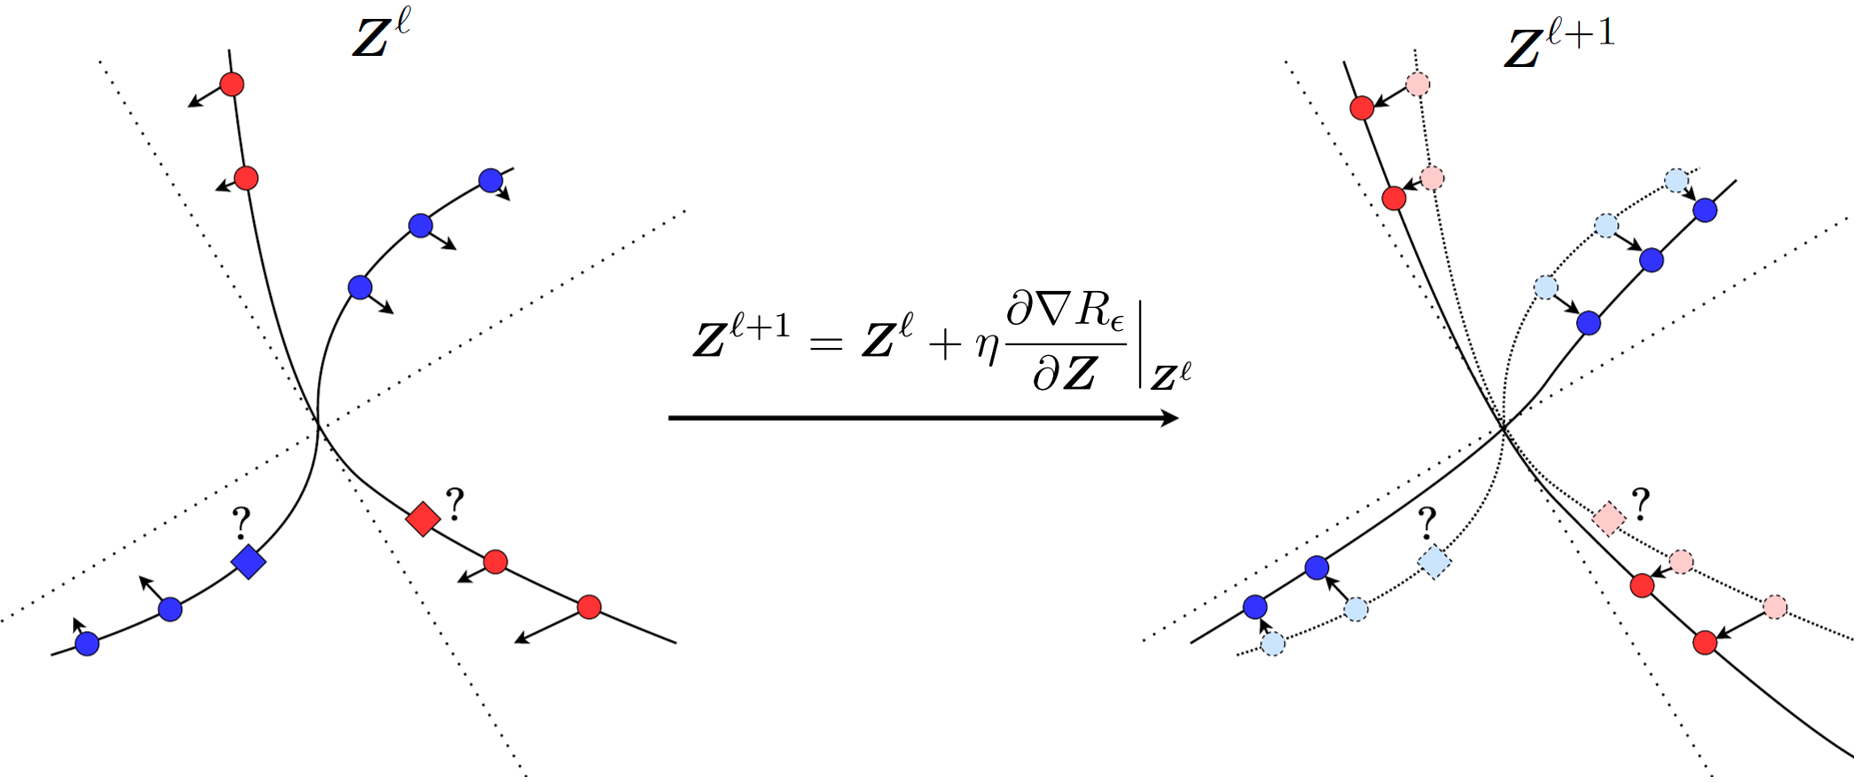
\includegraphics[width=0.85\linewidth]{\toplevelprefix/chapters/chapter4/figs/redu_gradient_diagram.png} 
    \caption{Incremental deformation via gradient flow to both flatten data of each class into a subspace and push different classes apart.} 
    \label{fig:gradient-flow}
\end{figure} 


Simple calculation shows that the gradient ${\partial \Delta R_{\epsilon}}/{\partial \bm Z}$ entails evaluating the following derivatives of the two terms in $\Delta R_{\epsilon}$:
\begin{equation}\label{eqn:expand-directions}
    \frac{1}{2}\frac{\partial \log \det (\I \!+\! \alpha \Z \Z^{\top} )}{\partial \bm Z}(\Z^\ell) = \underbrace{\alpha(\I \!+\! \alpha\Z^\ell (\Z^\ell)^\top)^{-1}}_{\bm E^{\ell} \; \in \Re^{d\times d}}\Z^\ell,
\end{equation}

\begin{equation}\label{eqn:compress-directions}
\frac{1}{2}\frac{\partial \left( \gamma_{k}  \log \det (\I + \alpha_{k} \Z \bm \Pi_k \Z^{\top} )  \right)}{\partial \bm Z}(\Z^\ell) = \gamma_{k}  \underbrace{ \alpha_{k}  (\I +  \alpha_{k} \Z^\ell \bm \Pi_k (\Z^\ell)^{\top})^{-1}}_{\bm C^{\ell}_k \; \in \Re^{d\times d}} \Z^{\ell} \bm \Pi_k.
\end{equation}
Notice that in the above, the matrix $\bm E^{\ell}$  only depends on $\Z^{\ell}$ and it aims to {\em expand} all the features to increase the overall coding rate; the matrix $\bm C^{\ell}_{k}$ depends on features from the $k$-class and aims to {\em compress} them to reduce the coding rate of each class. 
Then the complete gradient $\frac{\partial \Delta R_{\epsilon}}{\partial \bm Z}(\Z^\ell) \in \Re^{d\times N}$ is of the  form:
\begin{equation}
\frac{\partial \Delta R_{\epsilon}}{\partial \bm Z}(\Z^\ell)  = \underbrace{\bm E^{\ell}}_{\text{Expansion}} \Z^{\ell} \;-\; \sum_{k=1}^K \gamma_{k} \underbrace{\bm C_{k}^{\ell}}_{\text{Compression}}  \Z^{\ell} \bm{\Pi}_k.
\label{eqn:DR-gradient}
\end{equation}

\begin{remark}[Interpretation of $\bm E^\ell$ and $\bm C_j^\ell$ as linear operators]\label{rem:regression-interpretation} 
For any $\bm z^\ell \in \mathbb{R}^d$,
\begin{gather}
    \bm E^\ell \bm z^\ell = \alpha(\bm z^\ell - \bm Z^\ell \bm q^\ell_\star), \qquad
    \mbox{where} \qquad \bm q^\ell_\star \doteq \argmin_{\bm q^\ell} \big\{\alpha \|\bm z^\ell - \bm Z^\ell \bm q^\ell\|_2^2 + \|\bm q^\ell\|_2^2\big\}.
\end{gather}
Notice that $\bm q^\ell_\star$ is exactly the solution to the ridge regression by all the data points $\bm Z^\ell$ concerned. Therefore, $\bm E^\ell$ (similarly for $\bm C^\ell_k$) is approximately (i.e., when $N$ is large enough) the projection onto the orthogonal complement of the subspace spanned by columns of $\bm Z^\ell$. Another way to interpret the matrix $\bm E^\ell$ is through eigenvalue decomposition of the covariance matrix $\Z^\ell (\Z^\ell)^\top$. Assuming that $\Z^\ell (\Z^\ell)^\top \doteq \bm U^\ell \bm \Lambda^\ell (\bm U^\ell)^\top$ where $\bm \Lambda^\ell \doteq \diag\left(\lambda^\ell_1, \ldots, \lambda^\ell_d \right)$, we have 
\begin{equation}
\bm E^\ell = \alpha \bm U^\ell\, \diag\left(\frac{1}{1+\alpha\lambda^\ell_1}, \ldots, \frac{1}{1+\alpha\lambda^\ell_d}\right) \left(\bm U^\ell\right)^\top.
\end{equation}
Therefore, the matrix $\bm E^\ell$ operates on a vector $\bm z^\ell$ by stretching in a way that directions of large variance are shrunk while directions of vanishing variance are kept. These are exactly the directions \eqref{eqn:expand-directions} in which we move the features so that the overall volume expands and the coding rate will increase, hence the positive sign. To the opposite effect, the directions associated with \eqref{eqn:compress-directions} are ``residuals'' of features of each class deviate from the subspace to which they are supposed to belong. These are exactly the directions in which the features need to be compressed back onto their respective subspace, hence the negative sign (see Figure~\ref{fig:regression-interpretation}). 

\begin{figure}[t]
    \centering
    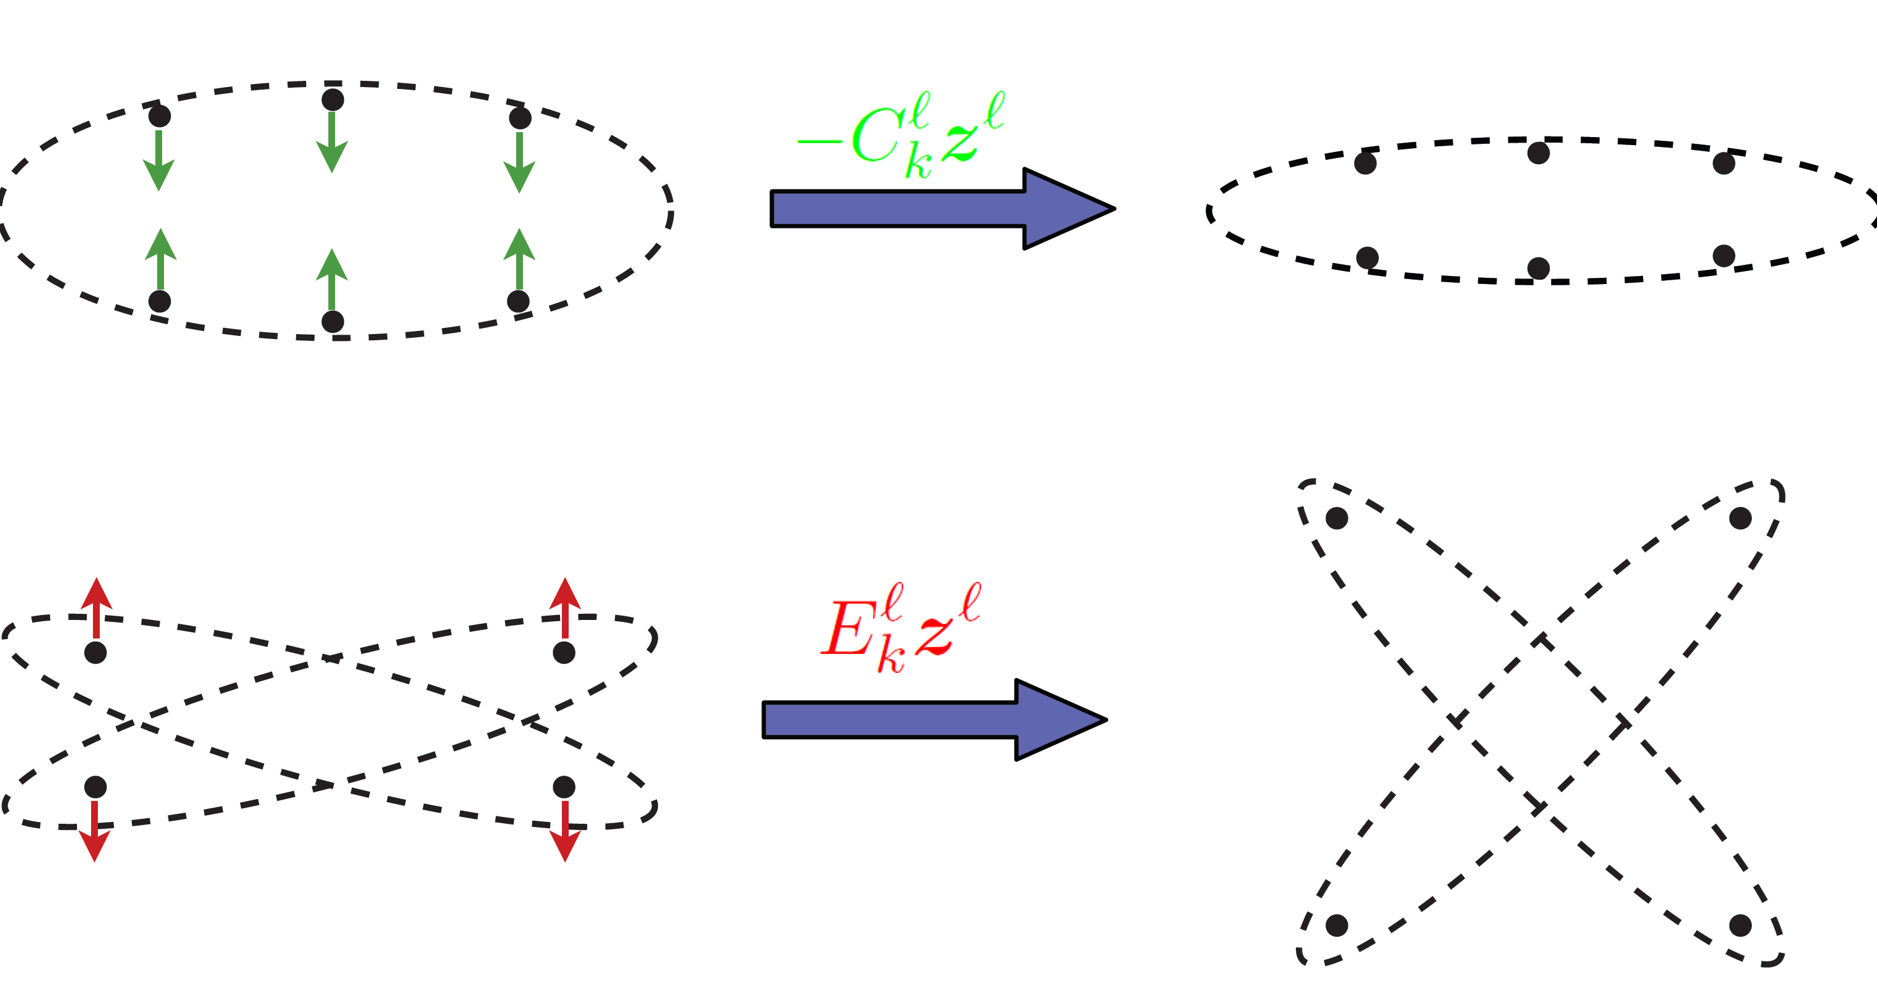
\includegraphics[width=0.65\linewidth]{\toplevelprefix/chapters/chapter4/figs/expand_compress.png}
    \caption{\small Interpretation of $\bm C^\ell_k$ and $\bm E^\ell$: $\bm C^\ell_k$ compresses each class by contracting the features to a low-dimensional subspace; $\bm E^\ell$ expands all features by contrasting and repelling features across different classes.}
    \label{fig:regression-interpretation}
    \vspace{-0.1in}
\end{figure}


Essentially, the linear operations $\bm E^\ell$ and $\bm C_k^\ell$ in gradient ascend for rate reduction are determined by training data conducting ``auto-regressions". The recent renewed understanding about ridge regression in an over-parameterized setting \cite{yang2020rethinking,Wu2020OnTO} indicates that using seemingly redundantly sampled data (from each subspace) as regressors does not lead to overfitting.
\end{remark}

\paragraph{Gradient-Guided Feature Map Increment.} Notice that in the above, the gradient ascent considers all the features $\Z^{\ell} = [\z^{\ell}_{1}, \dots, \z^{\ell}_{N}]$ as free variables. The increment $\Z^{\ell+1} - \Z^{\ell} = \eta \frac{\partial \Delta R_{\epsilon}}{\partial \bm Z}(\Z^\ell)$ does not yet give a transformation on the entire feature domain $\z^\ell \in \Re^d$. According to equation \eqref{eqn:DR-gradient}, the gradient cannot be evaluated at a point whose membership is not known, as illustrated in Figure \ref{fig:gradient-flow}. Hence, in order to find the optimal $f(\x,\bm  \theta)$ explicitly, we may consider constructing a small increment transform $g(\cdot, \bm{\theta}^{\ell})$ on the $\ell$-th layer feature $\z^\ell$ to emulate the above (projected) gradient scheme:
\begin{equation}
\z^{\ell + 1}   \; \propto \; \z^{\ell} + \eta\cdot  g(\z^{\ell}, \bm{\theta}^{\ell}) \quad \mbox{subject to} \quad \z^{\ell +1} \in \mathbb{S}^{d-1}
\label{eqn:gradient-descent-transform}
\end{equation}
such that $\big[g(\z_1^{\ell}, \bm \theta^{\ell}), \ldots, g(\z_N^{\ell}, \bm \theta^{\ell}) \big] \approx \frac{\partial \Delta R_{\epsilon}}{\partial \bm Z}(\Z^\ell).$ That is, we need to approximate the gradient flow $\frac{\partial \Delta R_{\epsilon}}{\partial \bm Z}$ that locally deforms all (training) features $\{\z_i^\ell\}_{i=1}^N$ with a continuous mapping $g(\z,\bm \theta)$ defined on the entire feature space $\z^\ell \in \Re^d$.  
Notice that one may interpret the increment \eqref{eqn:gradient-descent-transform} as a discretized version of a continuous  differential equation:
\begin{equation}
\dot{\z} = g(\z, \theta).
\end{equation}
Hence the (deep) network so constructed can be interpreted as certain neural ODE \cite{chen2018neural}. Nevertheless, unlike neural ODE where the flow $g$ is chosen to be some generic structures, here our $g(\z, \bm\theta)$ is to emulate the gradient flow of the rate reduction on the feature set (as shown in Figure \ref{fig:gradient-flow}): 
\begin{equation*}
    \dot{\Z} = \frac{\partial \Delta R_{\epsilon}}{\partial \bm Z},
\end{equation*} 
and its structure is entirely derived and fully determined from this objective, without any other priors or heuristics.  

By inspecting the structure of the gradient \eqref{eqn:DR-gradient}, it suggests that a natural candidate for the increment transform $g(\z^\ell, \bm \theta^\ell)$ is of the form:
\begin{equation}
    g(\z^\ell, \bm \theta^\ell) \; \doteq \; \bm E^\ell \z^\ell - \sum_{k=1}^K \gamma_{k} \pi_k(\z^\ell)\bm C_{k}^{\ell}  \z^{\ell}  \in \Re^d,
    \label{eqn:DR-gradient-transform}
\end{equation}
where $\pi_k(\z^\ell) \in [0,1]$ indicates the probability of $\z^{\ell}$ belonging to the $k$-th class. The increment map parameters $\bm \theta^\ell$ depend on: First, a set of linear maps represented by $\bm E^{\ell}$ and $\{ \bm C^{\ell}_{k}\}_{k=1}^{K}$ that depend only on statistics of features of the training $\Z^\ell$; Second, the membership $\{ \pi_k(\z^\ell)\}_{k=1}^K$ of any feature $\z^\ell$. 
Notice that on the training samples $\Z^\ell$, for which the memberships $\bm \Pi_k$ are known,  the so defined $g(\z^\ell, \bm \theta)$ gives exactly the values for the gradient $\frac{\partial \Delta R_{\epsilon}}{\partial \bm Z}(\Z^\ell)$.  


Since we only have the membership  for the training samples, the function $g(\cdot)$ defined in \eqref{eqn:DR-gradient-transform} can only be evaluated on the training. To extrapolate $g(\cdot)$ to the entire feature space, we need to estimate $\pi_k(\z^\ell)$ in its second term. In conventional deep learning, this map is typically modeled as a deep network and learned from the training data, say via {\em back propagation}. Nevertheless, our goal here is not to learn a precise classifier $\pi_{k}(\z^\ell)$ already. Instead, we only need a good enough estimate of the class information in order for $g(\cdot)$ to approximate the gradient $\frac{\partial \Delta R_{\epsilon}}{\partial \bm Z}$ well. 



From the geometric interpretation of the linear maps $\bm E^\ell$ and $\bm C_k^\ell$ given by Remark \ref{rem:regression-interpretation}, the term $\bm p_{k}^{\ell} \doteq \bm C^{\ell}_k \z^{\ell}$ can be viewed as (approximately) the projection of $\z^{\ell}$ onto the orthogonal complement of each class $j$. Therefore, $\|\bm p_{j}^{\ell}\|_2$ is small if $\z^\ell$ is in class $j$ and large otherwise. This motivates us to estimate its membership based on the following softmax function:
\begin{equation}
    \widehat{\vpi}(\z^\ell) \doteq \softmax\rp{-\lambda\mat{\norm{\vC^{\ell}_{1}\vz^{\ell}}_{2} \\ \vdots \\ \norm{\vC^{\ell}_{K}\vz^{\ell}}_{2}}} = \frac{1}{\sum_{k = 1}^{K}\exp(-\lambda \norm{\vC^{\ell}_{k}\vz^{\ell}}_{2})}\mat{\exp(-\lambda\norm{\vC^{\ell}_{1}\vz^{\ell}}_{2}) \\ \vdots \\ \exp(-\lambda\norm{\vC^{\ell}_{K}\vz^{\ell}}_{2})} \in [0,1]^{K}.
\end{equation}
Hence, the second term of \eqref{eqn:DR-gradient-transform} can be approximated by this estimated membership:
\begin{align}
\sum_{k=1}^K \gamma_{k} \pi_k(\z^\ell)\bm C_{k}^{\ell}  \z^{\ell} 
\; \approx \;  \sum_{k=1}^K \gamma_{k} \widehat{\pi}_k(\z^\ell)  \bm{C}^{\ell}_k  \z^{\ell} 
\; \doteq \; \bm \sigma\Big([\bm{C}^{\ell}_{1} \z^{\ell}, \dots, \bm{C}^{\ell}_{K} \z^{\ell}]\Big),
\label{eqn:soft-residual}
\end{align}
which is denoted as a nonlinear operator $\bm \sigma(\cdot)$ on outputs of the feature $\z^\ell$ through $K$ groups of filters: $[\bm{C}^{\ell}_{1}, \dots, \bm{C}^{\ell}_{K}]$. Notice that the nonlinearality arises due to a ``soft'' assignment of class membership based on the feature responses from those filters.  

Overall, combining \eqref{eqn:gradient-descent-transform},  \eqref{eqn:DR-gradient-transform}, and \eqref{eqn:soft-residual}, 
the increment feature transform from $\z^{\ell}$ to $\z^{\ell+1}$ now becomes
\begin{equation}\label{eqn:layer-approximate}
\begin{aligned}
\z^{\ell+1}  &\propto \; \z^\ell +  \eta \cdot  \bm E^{\ell} \z^{\ell} - \eta\cdot  \bm \sigma\big([\bm{C}^{\ell}_{1} \z^{\ell}, \dots, \bm{C}^{\ell}_{K} \z^{\ell}]\big)  \\
&= \; \z^\ell +  \eta \cdot g(\z^\ell, \bm \theta^\ell) \qquad \mbox{s.t.} \quad \z^{\ell +1} \in \mathbb{S}^{d-1},
\end{aligned}
\end{equation}
with the nonlinear function $\bm \sigma(\cdot)$ defined above and $\bm \theta^\ell$ collecting all the layer-wise parameters. That is  $\bm \theta^\ell =\left\{\bm E^\ell, \bm{C}^{\ell}_{1}, \dots, \bm{C}^{\ell}_{K}, \gamma_{k}, \lambda\right\}$. Note features at each layer are always ``normalized'' by projecting onto the unit sphere $\mathbb S^{d-1}$, denoted as $\mathcal P_{\mathbb S^{d-1}}$. The form of increment in \eqref{eqn:layer-approximate} can be illustrated by a diagram in  Figure~\ref{fig:arch-ReduNet}(a).

\begin{figure}[t]
    \begin{subfigure}[t]{0.35\textwidth}
        \centering
        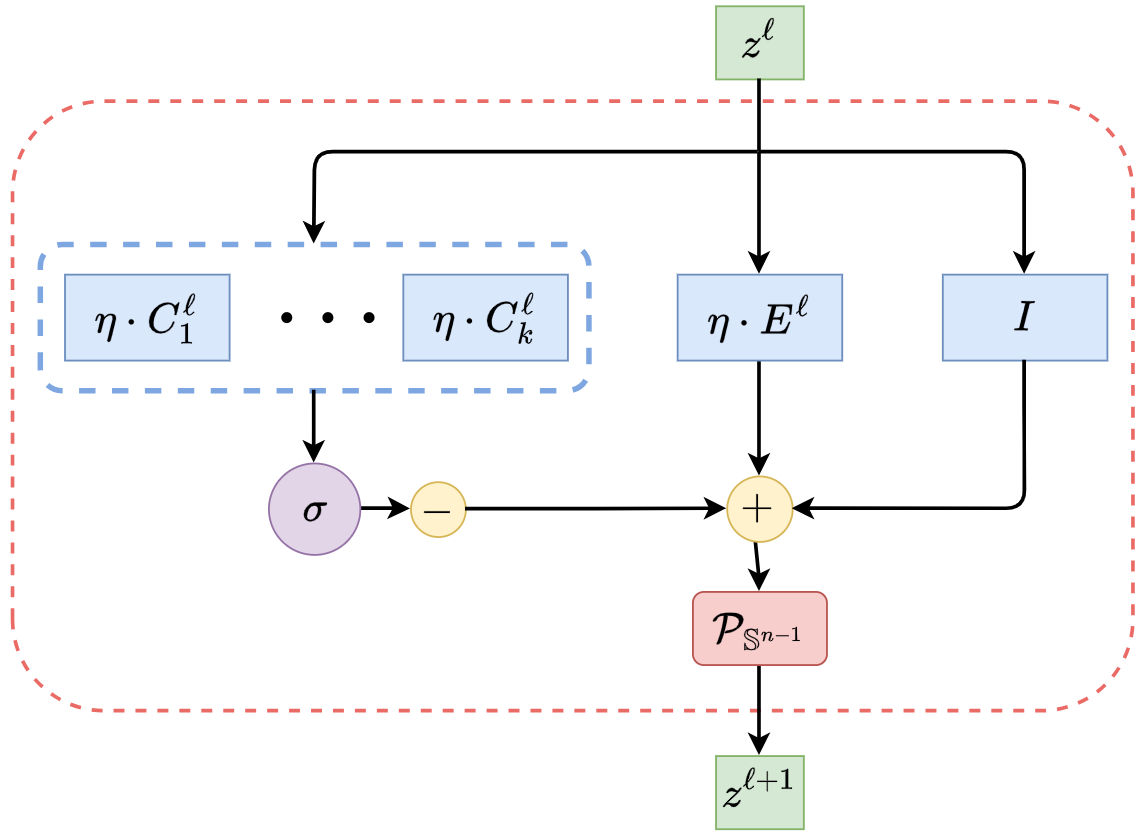
\includegraphics[width=\textwidth]{\toplevelprefix/chapters/chapter4/figs/redunet_layer.png}
        \caption{\textbf{ReduNet}}
    \end{subfigure}
    \hfill 
    \begin{subfigure}[t]{0.6\textwidth}
        \centering
        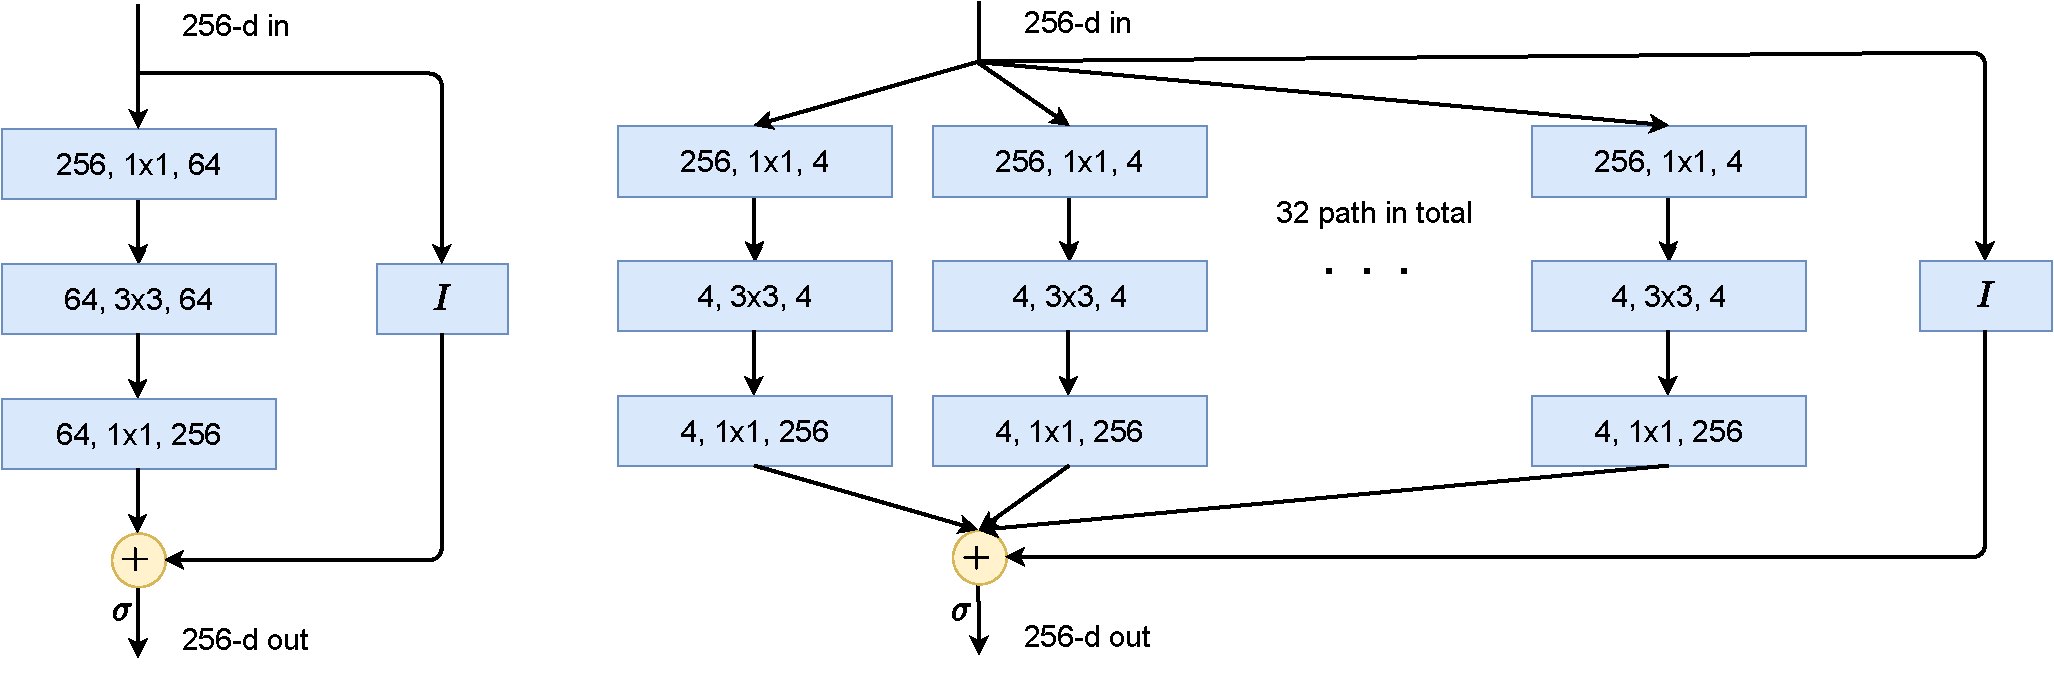
\includegraphics[width=\textwidth]{\toplevelprefix/chapters/chapter4/figs/resnet_resnext.pdf}
        \caption{\textbf{ResNet} and \textbf{ResNeXt}.}
    \end{subfigure}
    \caption{\small Network Architectures of the ReduNet and comparison with others. \textbf{(a)}: Layer structure of the \textbf{ReduNet} derived from one iteration of gradient ascent for optimizing rate reduction. \textbf{(b)} (left): A layer of ResNet~\cite{he2016deep}; and \textbf{(b)} (right): A layer of ResNeXt~\cite{ResNEXT}. As we will see in Section~\ref{sec:shift-invariant}, the linear operators $\bm E^\ell$ and $\bm{C}_k^\ell$ of the ReduNet naturally become (multi-channel) convolutions when shift-invariance is imposed.}
    \label{fig:arch-ReduNet}
\end{figure}

\begin{algorithm}[t]
    \caption{Training algorithm for ReduNet}
    \label{alg:redunet_training}
    \begin{algorithmic}[1]
        \Require{$\vX = [\vx_1, \ldots, \vx_N]\in \Re^{D \times N}$, $\bm{\Pi} = \{\bm \Pi_k\}_{k=1}^K$, $\epsilon > 0$, $\lambda$, and a learning rate $\eta$.}
        \Ensure{The learned parameters \(\{\vE^{\ell}\}_{\ell = 1}^{L}, \{\{\vC^{\ell}_{k}\}_{k = 1}^{K}\}_{\ell = 1}^{L}, \{\gamma_{k}\}_{k = 1}^{k}\)}

        \Procedure{ReduNetTraining}{$\vX, \vPi, \epsilon, \lambda, \eta$}
            \Statex{\quad\ \texttt{\# Define constants}}

            \State{\(\alpha \gets d/(N\epsilon^{2})\)}
            \For{\(k \in \{1, \dots, K\}\)}
            \State{\(\alpha_{k} \gets D/(\tr(\vPi_{k})\epsilon^{2})\)}
            \State{\(\gamma_{k} \gets \tr(\vPi_{k})/D\)}
            \EndFor
            \Statex{}

            \Statex{\quad\ \texttt{\# ReduNet layer-by-layer iteration}}
            \State{\(\vZ^{1} = \mat{\vz_{1}^1, \dots, \vz_{N}^1} \gets \vX\)} \Comment{Initialize the ReduNet per-layer iteration}
            \For{\(\ell \in \{1, \dots, L\}\)}
                \Statex{\quad\ \texttt{\# Step 1: Compute network parameters} \(\vE^{\ell}, \{\vC^{\ell}_{k}\}_{k = 1}^{K}\)}
                \State{\(\vE^{\ell} \gets \alpha\left(\vI + \alpha \vZ^{\ell}(\vZ^{\ell})^{\top}\right)^{-1} \in \R^{d \times d}\)}
                \For{\(k \in \{1, \dots, K\}\)}
                    \State{\(\vC^{\ell}_{k} \gets \alpha_{k}\left(\vI + \alpha_{k}\vZ^{\ell}\vPi_{k}(\vZ^{\ell})^{\top}\right)^{-1} \in \R^{d \times d}\)}
                \EndFor
                \Statex{}
                \Statex{\qquad\quad\texttt{\# Step 2: Update features \(\vZ^{\ell}\)}}
                \For{\(i \in \{1, \dots, N\}\)}
                    \State{\(\hat{\vpi}(\vz^{\ell}_i) \gets \displaystyle \softmax(-\lambda[\norm{\vC^{\ell}_{1}\vz^{\ell}_i}_{2}, \dots, \norm{\vC^{\ell}_{K}\vz^{\ell}_i}_{2}]) \in [0, 1]^{K}\)} \Comment{Compute soft assignments \(\hat{\vpi}(\vz^{\ell}_i)\)}
                    \State{\(\displaystyle\vz^{\ell + 1}_i \gets \cP_{\bS^{d - 1}}\rp{\vz^{\ell}_i + \eta \bp{\vE^{\ell}\vz^{\ell}_i - \sum_{k = 1}^{K}\gamma_{k}\hat{\pi}_{k}(\vz^{\ell}_i) \vC^{\ell}_{k}\vz^{\ell}_i}} \in \R^{d}\)} \Comment{Update features \(\vz^{\ell + 1}_i\) from \(\vz^{\ell}_i\)}
                \EndFor
            \EndFor
            \State{\Return{\(\{\vE^{\ell}\}_{\ell = 1}^{L}, \{\{\vC^{\ell}_{k}\}_{k = 1}^{K}\}_{\ell = 1}^{L}, \{\gamma_{k}\}_{k = 1}^{K}\)}} \Comment{Return all network parameters.}
        \EndProcedure
    \end{algorithmic}
\end{algorithm}


\paragraph{Deep Network for Optimizing Rate Reduction.} Notice that the increment is constructed to emulate the gradient ascent for the rate reduction $\Delta R_\epsilon$. Hence by transforming the features iteratively via the above process, we expect the rate reduction to increase, as we will see in the experimental section. This iterative process, once converged say after $L$ iterations, gives the desired feature map $f(\x, \bm \theta)$ on the input $\x = \z……0 $, precisely in the form of a {\em deep network}, in which each layer has the structure shown in Figure~\ref{fig:arch-ReduNet} left:
\begin{equation}\label{eqn:ReduNet}
\begin{aligned}
f(\x, \bm \theta)\; =&  \;\;f^L \circ f^{L-1} \circ  \cdots \circ f^1 \circ
    f^0(\z^0),  \\ 
f^\ell(\z^\ell, \bm \theta^\ell) \; \doteq & \;\; \z^{\ell+1} = \mathcal{P}_{\mathbb{S}^{n-1}}[\z^{\ell} + \eta\cdot g(\z^{\ell}, \bm \theta^{\ell})], \\
g(\z^{\ell}, \bm \theta^{\ell}) \; =&\;\; \bm E^{\ell} \z^{\ell} -  \bm \sigma\big([\bm{C}^{\ell}_{1} \z^{\ell}, \dots, \bm{C}^{\ell}_{K} \z^{\ell}]\big).
\end{aligned}
\end{equation}
As this deep network is derived from maximizing the rate \textbf{redu}cation, we call it the \textbf{ReduNet}. By comparing the architecture of ReduNet with those of popular empirically designed networks, \textbf{ResNet} and \textbf{NesNeXt} shown in Figure \ref{fig:arch-ReduNet}, the similarity is somewhat uncanny. Conceptually, ReduNet could also be used to justify the popular mixture of experts (\textbf{MoE}) architecture \cite{MoE} as each parallel channel, $\bm{C}^{\ell}_k$, can be viewed as an ``expert'' trained for each class of objects.

\begin{figure}[t]
    \centering
    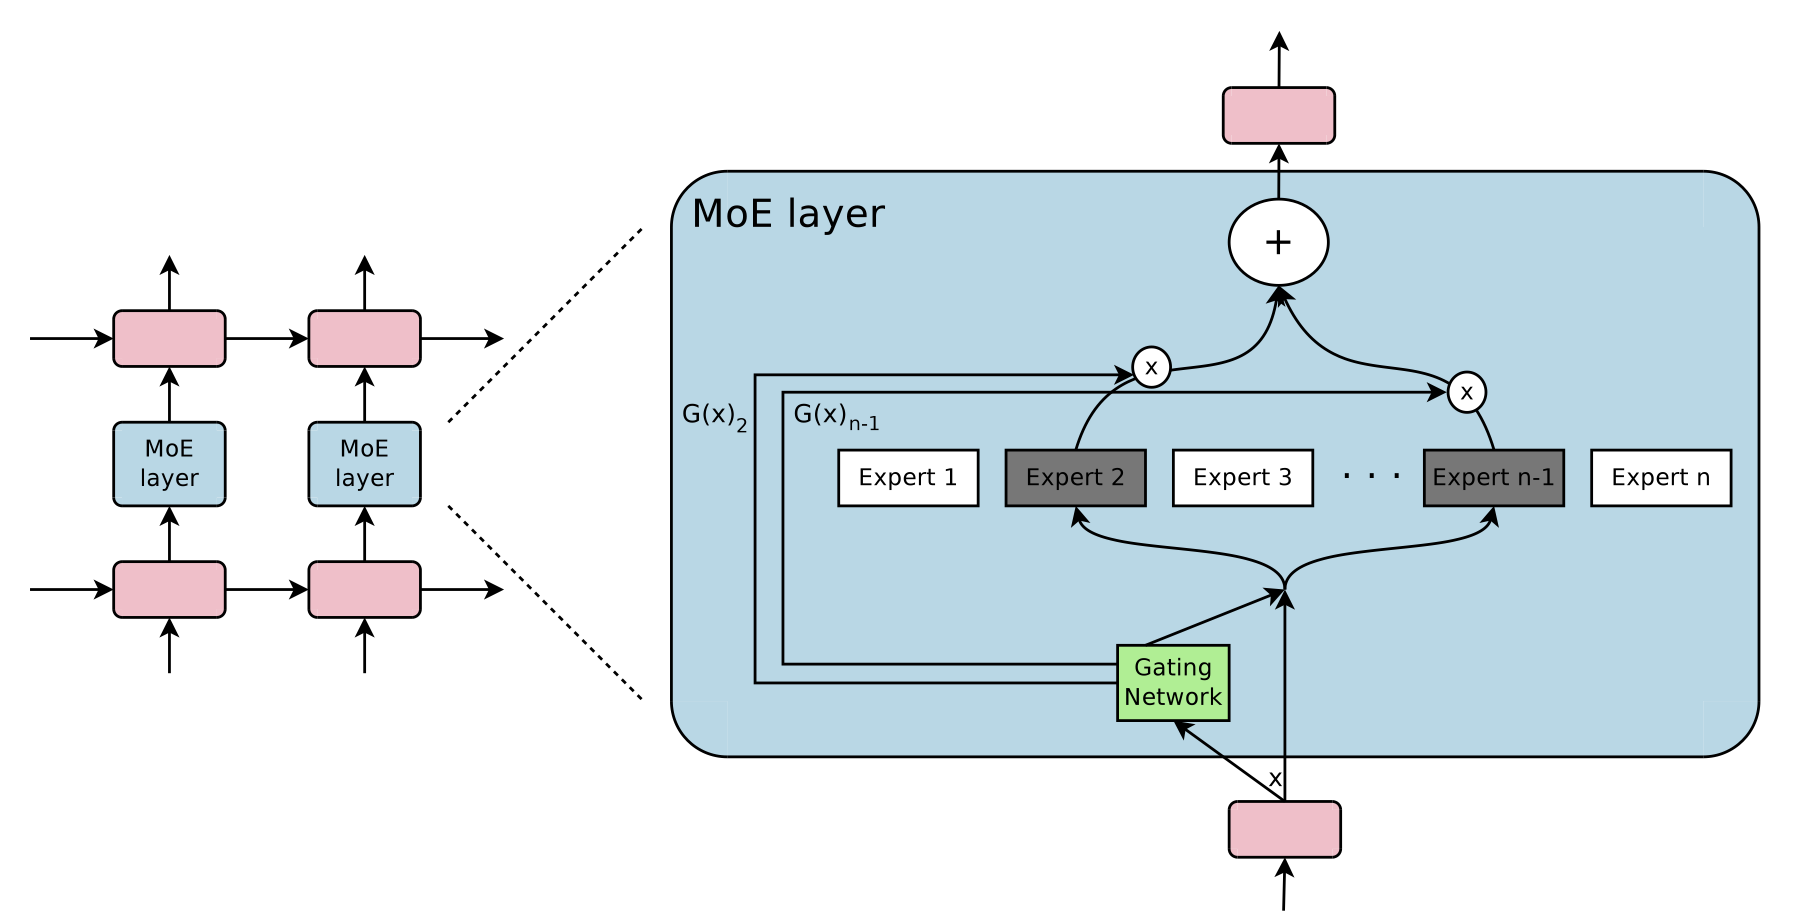
\includegraphics[width=0.45\linewidth]{\toplevelprefix/chapters/chapter4/figs/MoE.png} \hspace{5mm}
    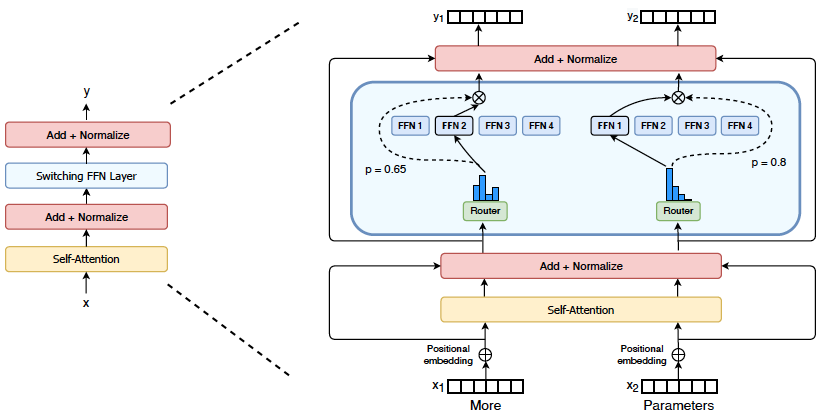
\includegraphics[width=0.45\linewidth]{\toplevelprefix/chapters/chapter4/figs/switched-transformer.png}
    \caption{Left: a mixture of experts (MoE) deep network \cite{MoE}. Right: a sparsity-promoting Switch Transformer \cite{Fedus-2022}, used to implement MoE with 1.7 trillion parameters.}
    \label{fig:enter-label}
\end{figure}

We summarize the training and evaluation of ReduNet in \Cref{alg:redunet_training} and \Cref{alg:redunet_evaluation}, respectively.  Notice that all parameters of the network are explicitly constructed layer by layer in a {\em forward propagation} fashion. The construction does not need any back propagation! The so-learned features can be directly used for classification, say via a nearest subspace classifier. 



\begin{algorithm}[!htbp]
    \caption{Evaluation algorithm for ReduNet}
    \label{alg:redunet_evaluation}
    \begin{algorithmic}[1]
        \Require{Input \(\vx \in \R^{D}\), network parameters \(\{\vE^{\ell}\}_{\ell = 1}^{L}, \{\{\vC^{\ell}_{k}\}_{k = 1}^{K}\}_{\ell = 1}^{L}, \{\gamma_{k}\}_{k = 1}^{K}\), learning rate \(\lambda\)}
        \Ensure{feature \(\vz^{L + 1}\)}

        \Procedure{ReduNetEvaluation}{$\vx$}
        \State{\(\vz^{1} \gets \vx \in \R^{D}\)} \Comment{Initialize the ReduNet per-layer iteration}
        \For{\(\ell \in \{1, \dots, L\}\)}
        \State{\(\hat{\vpi}(\vz^{\ell}) \gets  \softmax(-\lambda\mat{\norm{\vC^{\ell}_{1}\vz^{\ell}}_{2}, \dots, \norm{\vC^{\ell}_{K}\vz^{\ell}}_{2}}) \in [0, 1]^{K}\)} \Comment{Compute soft assignments \(\hat{\vpi}(\vz^{\ell})\)}
        \State{\(\vz^{\ell + 1} \gets \cP_{\bS^{d - 1}}\rp{\vz^{\ell} + \eta \bp{\vE^{\ell}\vz^{\ell} - \sum_{k = 1}^{K}\gamma_{k}\hat{\pi}_{k}(\vz^{\ell}) \vC^{\ell}_{k}\vz^{\ell}}} \in \R^{d}\)} \Comment{Update feature \(\vz^{\ell + 1}\) using \(\vz^{\ell}\)}
        \EndFor
        \State{\Return{\(\vz^{L + 1}\)}} \Comment{Return the output features}
        \EndProcedure
    \end{algorithmic}
\end{algorithm}


\begin{example}
To provide some intuition on how ReduNet transforms the features, we provide a simple example with mixed 3D Gaussians and visualize how the features are transformed in Figure~\ref{fig:redu-3d-gaussian-diagram}. 
Consider a mixture of three Gaussian distributions in $\R^{3}$ that is projected onto $\mathbb{S}^2$. We first generate data points for 3 classes: for $k=1,2,3$, $\bm{X}_{k}=[\bm{x}_{k,1}, \ldots, \bm{x}_{k,m}] \in \R^{3\times m}$, $\bm{x}_{k,i} \sim \mathcal{N}(\bm{\mu}_{k}, \sigma_{k}^{2} \I)$, and ${\pi}(\x_{k,i}) = k$.
We set $m=500, \sigma_{1}=\sigma_{2}=\sigma_{3}=0.1$, and $\bm{\mu}_{1}, \bm{\mu}_{2}, \bm{\mu}_{3} \in \mathbb{S}^2$. 
Then we project all the data points onto $\mathbb{S}^{2}$, i.e., $\bm{x}_{k,i}/\|\bm{x}_{k,i}\|_{2}$. 
To construct the network (computing $\bm{E}^{\ell}, \bm{C}^{\ell}_{k}$ for the $\ell$-th layer), we set the number of iterations/layers $L=2,000$, step size $\eta=0.5$, and precision $\epsilon=0.1$. 
We do this only to demonstrate that our framework leads to stable deep networks even with thousands of layers. 
In practice, thousands of layers may not be necessary and one can stop whenever adding new layers gives diminishing returns. 
For this example, a couple of hundred layers is sufficient. Hence, the clear optimization objective gives a natural criterion for the depth of the network needed.

As shown in \Cref{fig:redu-3d-gaussian-diagram}, we can observe that after the mapping $f(\cdot, \bm{\theta})$, samples from the same class are highly compressed and converge to a single cluster and the angle between two different clusters is approximately $\pi/2$, which is well aligned with the optimal solution $\Z^{\star}$ of the MCR$^2$ loss in $\mathbb{S}^2$. 
MCR$^2$ loss of features on different layers can be found in Figure~\ref{fig:redu-3d-gaussian-diagram}(\textbf{c}). Empirically, we find that the constructed ReduNet is able to maximize MCR$^2$ loss and converges stably and samples from the same class converge to one cluster and different clusters are orthogonal to each other. 
Moreover, when sampling new data points from the same distributions, we find that new samples from the same class consistently converge to the same cluster center as the training samples. 
\begin{figure}[t]
    \begin{subfigure}[t]{0.32\textwidth}
        \centering 
        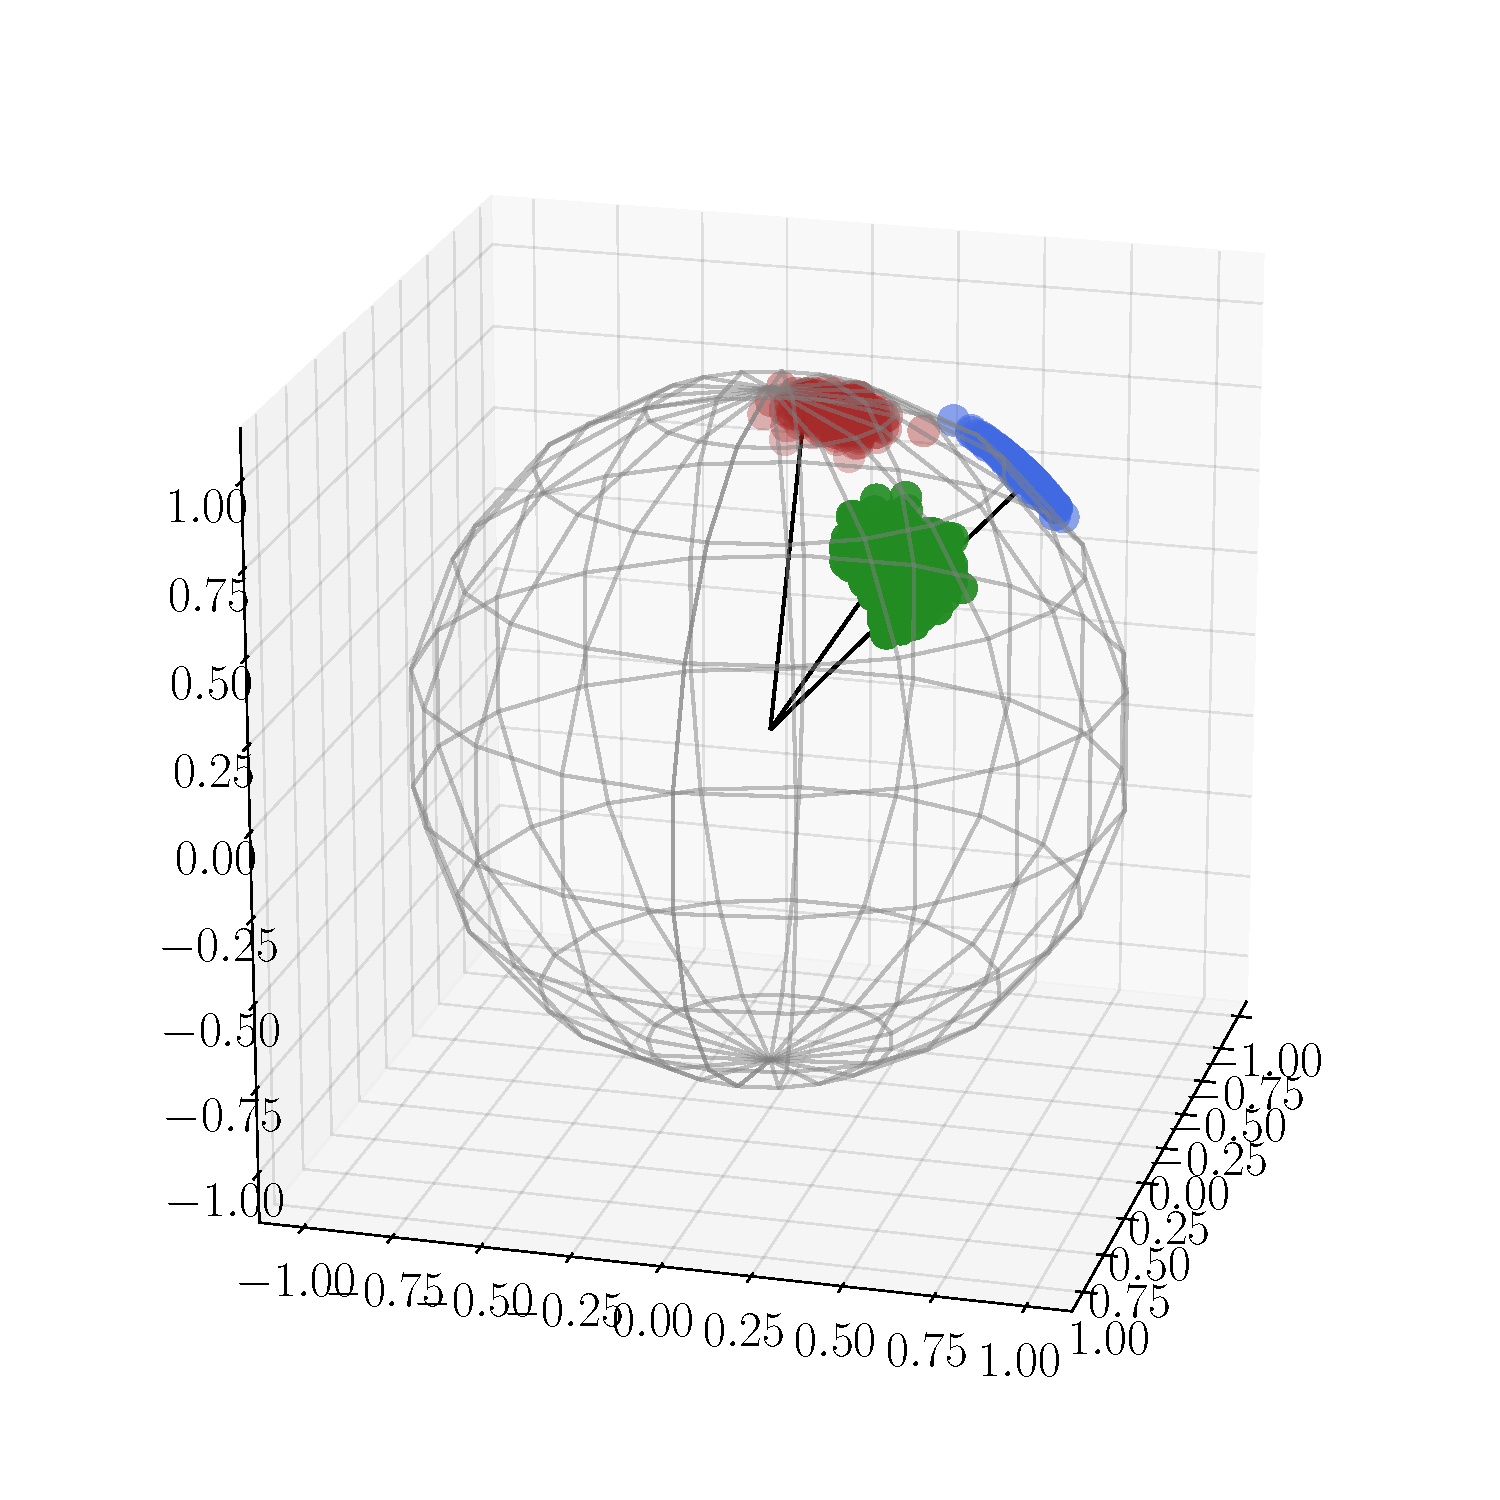
\includegraphics[width=\textwidth]{\toplevelprefix/chapters/chapter4/figs/scatter3d-X_train.pdf}\vspace{-0.1in}
        \caption{$\bm{X}_{\text{train}}$}
    \end{subfigure}
    \hfill
    \begin{subfigure}[t]{0.32\textwidth}
        \centering 
        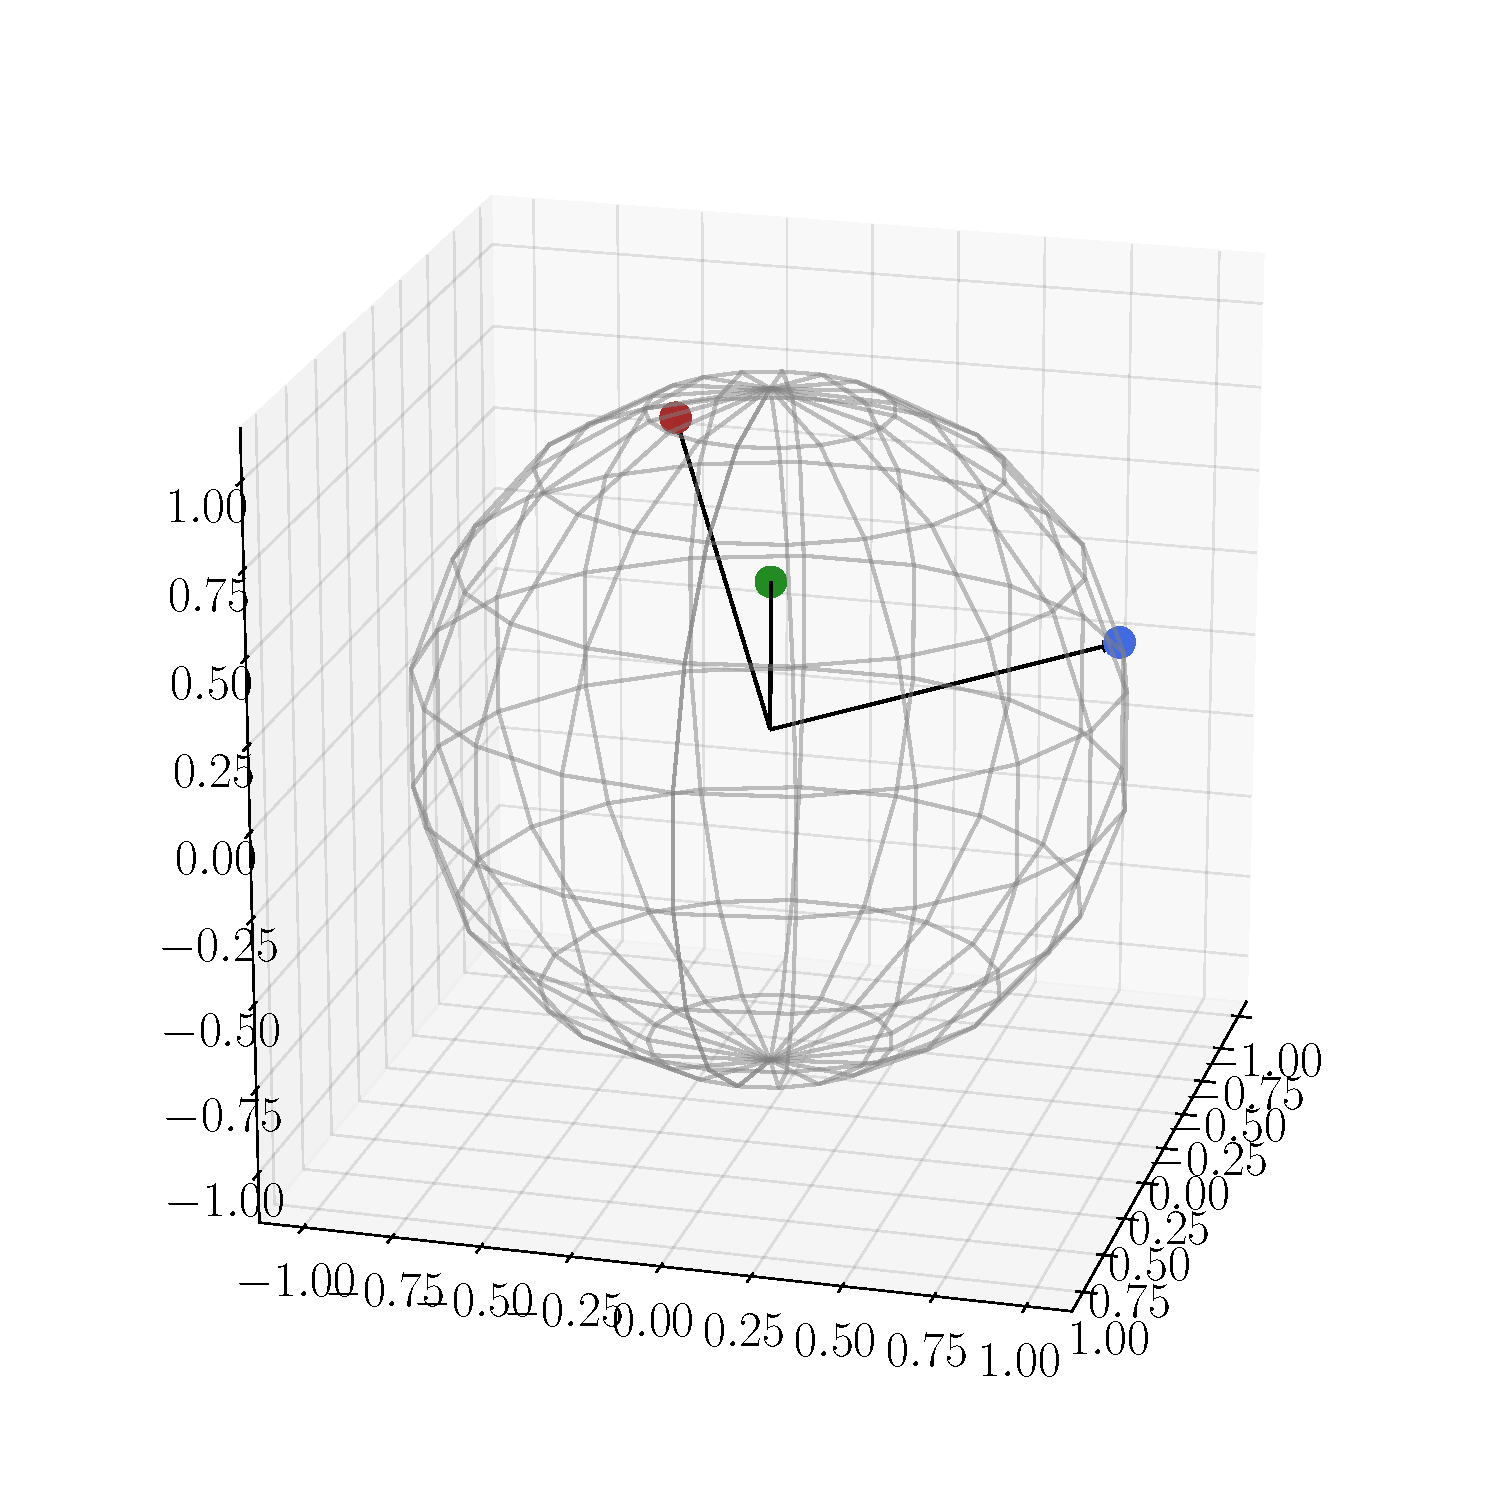
\includegraphics[width=\textwidth]{\toplevelprefix/chapters/chapter4/figs/scatter3d-Z_train.pdf}\vspace{-0.1in}
        \caption{$\bm{Z}_{\text{train}}$}
    \end{subfigure}
    \hfill
    \begin{subfigure}[t]{0.32\textwidth}
        \centering 
        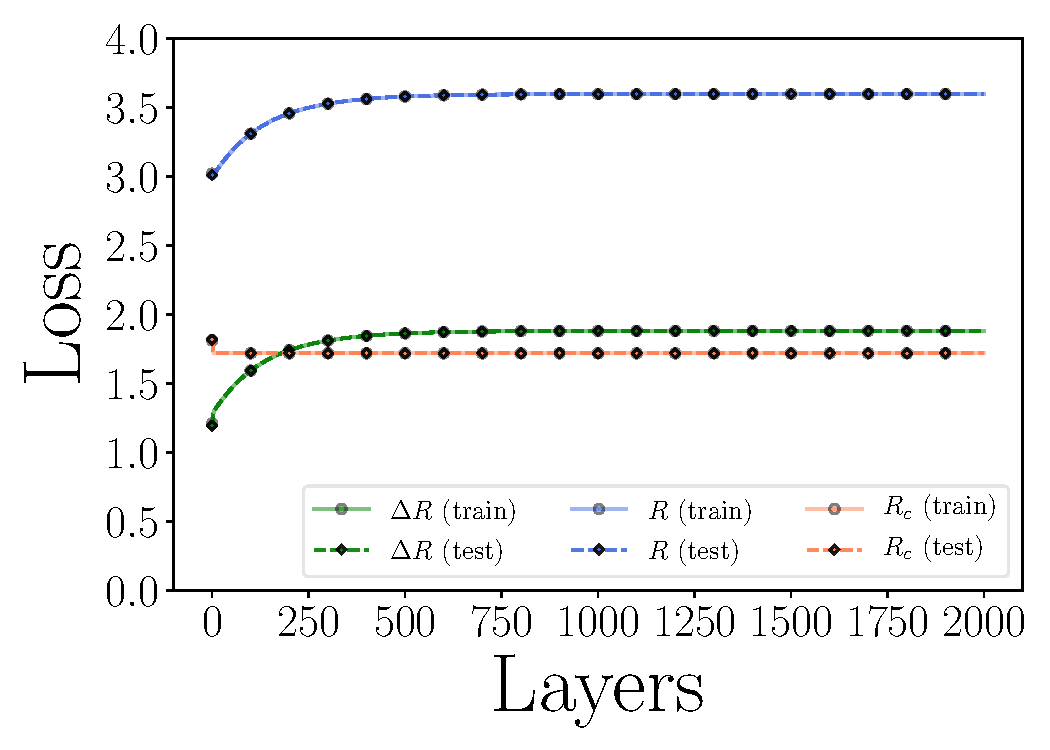
\includegraphics[width=\textwidth]{\toplevelprefix/chapters/chapter4/figs/scatter3d-loss-traintest.pdf}\vspace{-0.1in}
        \caption{Loss (train/val)}
    \end{subfigure}
    \vspace{-0.1in}
    \caption{\small Original samples  and learned representations for 3D Mixture of Gaussians. We visualize data points $\bm{X}$ (before mapping $f(\cdot, \bm{\theta})$) in (\textbf{a}) and learned features $\bm{Z}$ (after mapping $f(\cdot, \bm{\theta})$) in (\textbf{b}) by scatter plot. In each scatter plot, each color represents one class of samples. In (\textbf{c}), we also show the plots for the progression of values of the objective functions.}
    \label{fig:redu-3d-gaussian-diagram}
\end{figure}

\end{example}

\subsection{Convolutional Networks from Invariant Rate Reduction}\label{sec:shift-invariant}

In the previous section, we derived the layer-wise architecture of a deep network, the ReduNet, using unrolled optimization for the rate reduction objective. 
Specifically, the compression term $R^c_\epsilon(\Z \mid\bm \Pi)$ in \eqref{eq:mcr-formulation} is designed to compress representations from the same class. However, this formulation does not account for possible domain transformation or deformation of the input data. For instance, shifting an object slightly to the right does not change the semantic label of an image.  In this section, we will demonstrate how convolutional layers can be derived by maximizing a rate reduction objective that is invariant to certain domain deformations, such as image rotations and translations. 


For many clustering or classification tasks (such as object detection in images), we consider two samples as {\em equivalent} if they differ by certain classes of domain deformations or augmentations $\cT = \{\tau \}$. Hence, we are only interested in low-dimensional structures that are {\em invariant} to such deformations~(i.e., $\x \in \mathcal{M}$ iff $\tau(\x) \in \mathcal{M}$ for all $\tau \in \cT$\,), 
which are known to have sophisticated geometric and topological structures and can be difficult to learn precisely in practice, even with rigorously designed CNNs \cite{Cohen-ICML-2016}. 
In this framework, this can be formulated in a very natural way: all equivariant instances are to be embedded into the same subspace, so that the subspace itself is invariant to the transformations under consideration.

In many applications, such as serial data or imagery data, the semantic meaning (labels) of the data are  {\em invariant} to certain transformations $\mathfrak{g} \in \mathbb{G}$ (for some group $\mathbb{G}$) \cite{CohenW16,deep-sets-NIPS2017}. For example, the meaning of an audio signal is invariant to shift in time; and the identity of an object in an image is invariant to translation in the image plane. Hence, we prefer the feature mapping $f(\x,\bm \theta)$ is rigorously invariant to such transformations:
\begin{equation}
\mbox{\em Group Invariance:}\;   f(\x\circ \mathfrak{g}, \bm \theta) \sim f(\x,\bm \theta),\ \forall \mathfrak{g} \in \mathbb{G},
\end{equation}
where ``$\sim$'' indicates two features belonging to the same equivalent class. Although to ensure invariance or equivarience, convolutional operators have been common practice in deep networks \cite{CohenW16}, it remains challenging in practice to train an (empirically designed) convolution network from scratch that can {\em guarantee} invariance even to simple transformations such as translation and rotation \cite{azulay2018deep,engstrom2017rotation}. An alternative approach is to carefully design convolution filters of each layer so as to ensure translational invariance for a wide range of signals, say using wavelets as in ScatteringNet \cite{scattering-net} and followup works \cite{Wiatowski-2018}. However, in order to ensure invariance to generic signals, the number of convolutions needed usually grows exponentially with network depth. That is the reason why this type of network cannot be constructed so deep, usually only several layers. 

Now, we show that the MCR$^2$ principle is compatible with invariance in a natural and precise way: we only need to assign all transformed versions $\{\x\circ \mathfrak{g} \mid \mathfrak{g} \in \mathbb G\}$  into the same class as the data $\x$ and map their features $\z$ all to the same subspace $\mathcal S$. Hence, all group equivariant information is encoded only inside the subspace, and any classifier defined on the resulting set of subspaces will be automatically invariant to such group transformations. See Figure \ref{fig:ortho-invariance-diagram} for an illustration of the examples of 1D rotation and 2D translation.  Next, we will rigorously show that when the group $\mathbb G$ is circular 1D shifting, the resulting deep network naturally becomes a {\em multi-channel convolution network}. 
Because the so-constructed network only needs to ensure invariance for the given data $\X$ or their features $\Z$, the number of convolutions needed actually remains constant through a very deep network, as opposed to the ScatteringNet. 

\begin{figure}[t]
    \begin{subfigure}[t]{0.4\textwidth}
        \centering 
        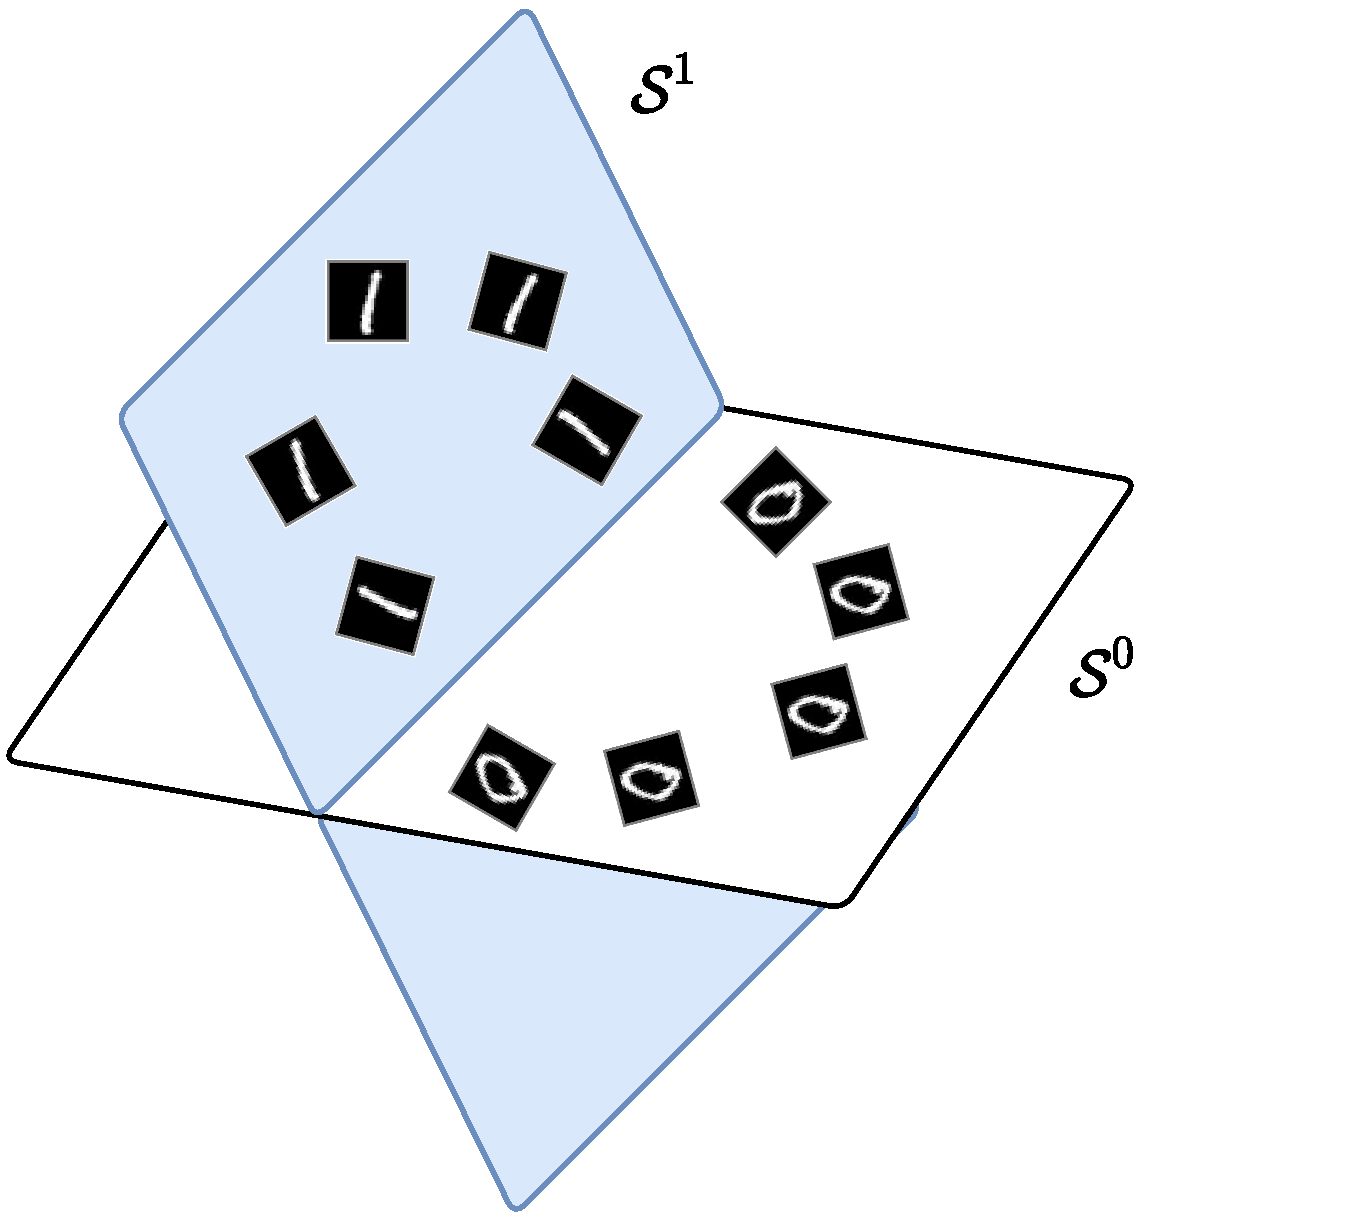
\includegraphics[width=\textwidth]{\toplevelprefix/chapters/chapter4/figs/ortho_diagram_1d.pdf}
    \end{subfigure}
    \hfill 
    \begin{subfigure}[t]{0.4\textwidth}
        \centering 
        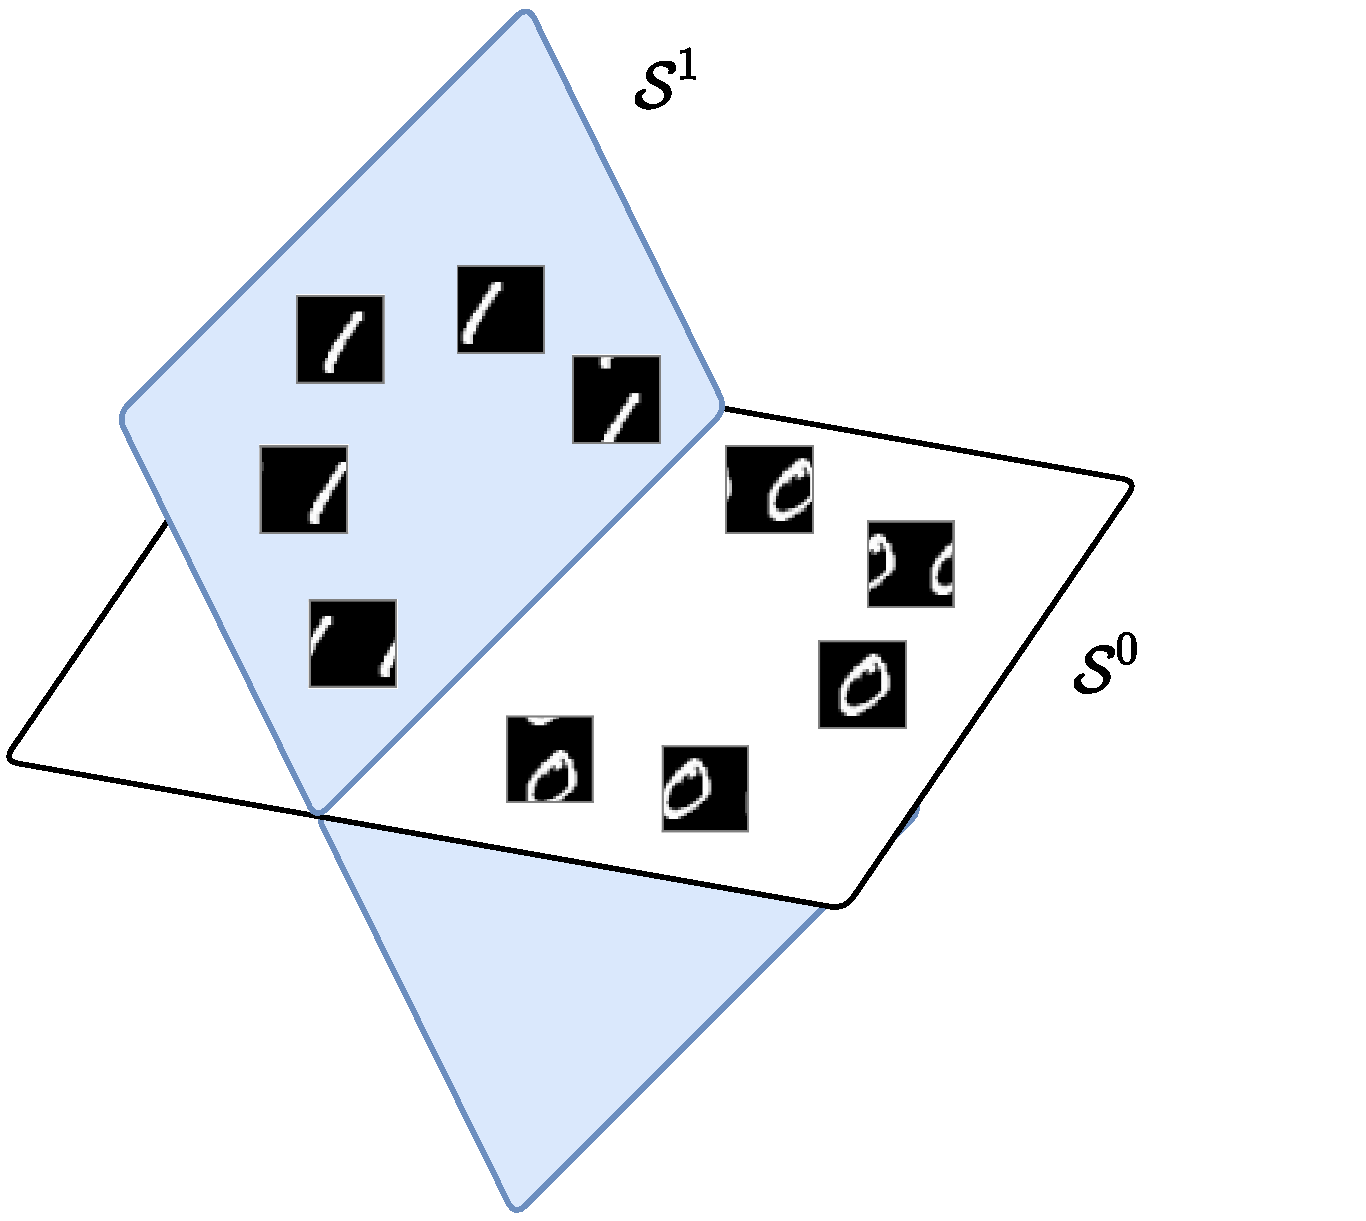
\includegraphics[width=\textwidth]{\toplevelprefix/chapters/chapter4/figs/ortho_diagram_2d.pdf}
    \end{subfigure}
    \caption{Illustration of the sought representation that is equivariant/invariant to image rotation (left) or translation (right): all transformed images of each class are mapped into the same subspace that is incoherent to other subspaces. The features embedded in each subspace are equivariant to the transformation group whereas each subspace is invariant to such transformations.}\label{fig:ortho-invariance-diagram} 
\end{figure}

\paragraph{1D Serial Data and  Shift Invariance} To classify one-dimensional data $\bm x = [x(0), x(1), \ldots, x(D-1)] \in \Re^D$ invariant under shifting, we take $\mathbb{G}$ to be the group of all circular shifts. Each observation $\bm x_i$ generates a family $\{ \x_i \circ \mathfrak{g} \, | \, \mathfrak{g} \in \mathbb G \}$ of shifted copies, which are the columns of the circulant matrix $\circm(\bm x_i) \in \Re^{D \times D}$ given by
\begin{equation}
\circm(\x) \,\doteq\, \left[ \begin{array}{ccccc} x(0) & x(D-1) & \dots & x(2) & x(1) \\ x(1) & x(0) & x(D-1) & \cdots & x(2) \\ \vdots & x(1) & x(0) &\ddots & \vdots \\ x(D-2) &  \vdots & \ddots & \ddots & x(D-1) \\ x(D-1) & x(D-2) & \dots & x(1) & x(0)   \end{array} \right]  \in \Re^{D \times D}.
\end{equation}
We refer the reader to \cite{Kra2012OnCM} for properties of circulant matrices. For simplicity, let $\bm Z^1 \doteq [ \z_{1}^1, \dots, \z_{N}^1 ] = \X \in \Re^{d \times N}$.\footnote{Again, to simplify discussion, we assume for now that the initial features $\Z^1$ are $\X$ themselves hence have the same dimension $d$, i.e., $D=d$. But that does not need to be the case as we will soon see that we need to lift $\X$ to a higher dimension.} Then what happens if we construct the ReduNet from their circulant families $\circm(\bm Z^1) = \left[ \circm(\z_{1}^1), \dots, \circm(\z_{N}^1) \right] \in \Re^{d \times (dN)}$? That is, we want to compress and map all these into the same subspace by the ReduNet. 

Notice that now the data covariance matrix: 
\begin{eqnarray}
\circm(\bm Z^1) \circm(\bm Z^1)^\top 
&=& \left[ \circm(\z_{1}^1), \dots, \circm(\z_{N}^1) \right] \left[ \circm(\z_{1}^1), \dots, \circm (\z_{N}^1) \right]^\top \nonumber \\
&=& \sum_{i =1}^N \circm(\z_{i}^1) \circm(\z_{i}^1)^\top \;\in \Re^{d\times d} 
\end{eqnarray}
associated with this family of samples is {\em automatically} a (symmetric) circulant matrix. Moreover, because the circulant property is preserved under sums, inverses, and products, the matrices $\bm E^1$ and $\bm C^1_k$ are also automatically circulant matrices, whose application to a feature vector $\bm z \in \Re^d$ can be implemented using circular convolution ``$\circledast$''.
Specifically, we have the following proposition. 

\begin{proposition}[Convolution structures of $\bm E^1$ and $\bm C^1_k$]
The matrix 
\begin{equation}
    \bm E^1 = \alpha\big(\bm I + \alpha \circm(\bm Z^1) \circm(\bm Z^1)^\top \big)^{-1}
\end{equation}
is a circulant matrix and represents a circular convolution: 
$$\bm E^1 \z = \bm e_1 \circledast \z,$$ 
where $\bm e_1 \in \Re^d$ is the first column vector of $\bm E^1$ and ``$\circledast$'' is circular convolution defined as
\begin{equation*}
    (\bm e_1 \circledast \bm z)_{i} \doteq \sum_{j=0}^{d-1} e_1(j) x(i+ d-j \,\, \textsf{mod} \,\,d).
\end{equation*}
Similarly, the matrices $\bm C^1_k$ associated with any subsets of $\bm Z^1$ are also circular convolutions. 
\label{prop:circular-conv-1}
\end{proposition}

Not only do the first-layer parameters $\bm E^1$ and $\bm{C}^1_k$ of the ReduNet become circulant convolutions but also the next-layer features remain circulant matrices. 
That is, the incremental feature transform in \eqref{eqn:layer-approximate} applied to all shifted versions of a $\z^1 \in \Re^d$, given by
\begin{equation}
    \circm(\z^1) + \eta \cdot \bm E^1 \circm(\z^1) - \eta \cdot \bm \sigma \Big([\bm{C}_1^1 \circm(\z^1), \ldots, \bm{C}^1_K \circm(\z^1)] \Big),
\end{equation}
is a circulant matrix.  This implies that there is no need to construct circulant families from the second layer features as we did for the first layer. 
By denoting
\begin{equation}
\z^{2} \propto \z^{1} +\eta \cdot g(\z^{1}, \bm \theta^{1}) =  \z^1 + \eta \cdot \bm e_{1} \circledast \z^{1} -  \eta \cdot \bm \sigma\Big([\bm{c}_{1}^{1} \circledast \z^{1}, \dots, \bm{c}^{1}_{K} \circledast \z^{1}]\Big),
\label{eqn:approximate-convolution}
\end{equation}
the features at the next level can be written as
$$\circm(\bm Z^2) = \big[ \circm( \bm z_{1}^1 + \eta g( \bm z_{1}^1, \bm \theta^1)), \dots, \circm( \bm z_{N}^1 + \eta g(\bm z_{N}^1, \bm \theta^1)) \big].$$
Continuing inductively, we see that all matrices $\bm E^\ell$ and $\bm C^\ell_k$ based on such $\circm(\bm Z^\ell)$ are circulant, and so are all features. 
By virtue of the properties of the data, ReduNet has taken the form of a convolutional network, {\em with no need to explicitly choose this structure!} 

\paragraph{A Fundamental Trade-off between Invariance and Sparsity.} 
There is one problem though: In general, the set of all circular permutations of a vector $\z$ gives a full-rank matrix. That is, the $d$ ``augmented'' features associated with each sample (hence each class) typically already span the entire space $\Re^d$. For instance, all shifted versions of a delta function $\delta(d)$ can generate any other signal as their (dense) weighted superposition. The MCR$^2$ objective \eqref{eqn:maximal-rate-reduction} will not be able to distinguish classes as different subspaces.

One natural remedy is to improve the separability of the data by ``lifting'' the original signal to a higher dimensional space, e.g., by taking their responses to multiple, filters $\bm k_1, \ldots, \bm k_C \in \Re^d$: 
\begin{equation}
\bm z[c] = \bm k_c \circledast \bm x  =  \circm(\bm k_c) \bm x \in \Re^d, \quad c = 1, \ldots, C.
\label{eqn:lift-1d}
\end{equation} 
The filters can be pre-designed invariance-promoting filters,\footnote{For 1D signals like audio, one may consider the conventional short-time Fourier transform (STFT); for 2D images, one may consider 2D wavelets as in the ScatteringNet \cite{scattering-net}.} or adaptively learned from the data,\footnote{For learned filters, one can learn filters as the principal components of samples as in the PCANet \cite{chan2015pcanet} or from convolution dictionary learning \cite{li2019multichannel,qu2019nonconvex}.} or randomly selected as we do in our experiments. This operation lifts each original signal $\x \in \Re^d$ to a $C$-channel feature, denoted as $\bar{\z}  \doteq [\z[1], \ldots, \z[C]]^\top \in \Re^{C\times d}$. 
Then, we may construct the ReduNet on vector representations of $\bar{\z}$, denoted as
$\vec(\bar\z) \doteq [\z[1]^\top, \ldots, \z[C]^\top] \in \Re^{dC}$. 
The associated circulant version $ \circm(\bar{\z})$ and its data covariance matrix, denoted as $\bar{\bm \Sigma}(\bar\z)$, for all its shifted versions are given as:
\begin{equation}
\begin{aligned}
 \circm(\bar{\z}) \doteq \left[\begin{matrix}
    \circm(\z[1])  \\ \vdots \\ \circm(\z[C]) \end{matrix} \right] \in \Re^{dC\times d}, 
    \quad  \bar{\bm \Sigma}(\bar\z) \doteq 
    \left[\begin{matrix}
    \circm(\z[1]) \\ \vdots \\ \circm(\z[C]) \end{matrix} \right]
    \left[\begin{matrix}\circm(\z[1])^\top,\ldots, \circm(\z[C])^\top\end{matrix} \right] \in \Re^{dC\times dC},
    \label{eqn:W-multichannel}
\end{aligned}
\end{equation}
where $\circm(\z[c]) \in \Re^{d\times d}$ with $c \in [C]$ is the circulant version of the $c$-th channel of the feature $\bar \z$. Then the columns of $\circm(\bar\z)$  will only span at most a $d$-dimensional proper subspace in $\Re^{dC}$.  However, this simple lifting operation (if linear) is not sufficient to render the classes separable yet---features associated with other classes will span the {\em same} $d$-dimensional subspace. This reflects a fundamental conflict between invariance and linear (subspace) modeling: {\em one cannot hope for arbitrarily shifted and superposed signals to belong to the same class.} 

\begin{figure}[t]
	\centerline{
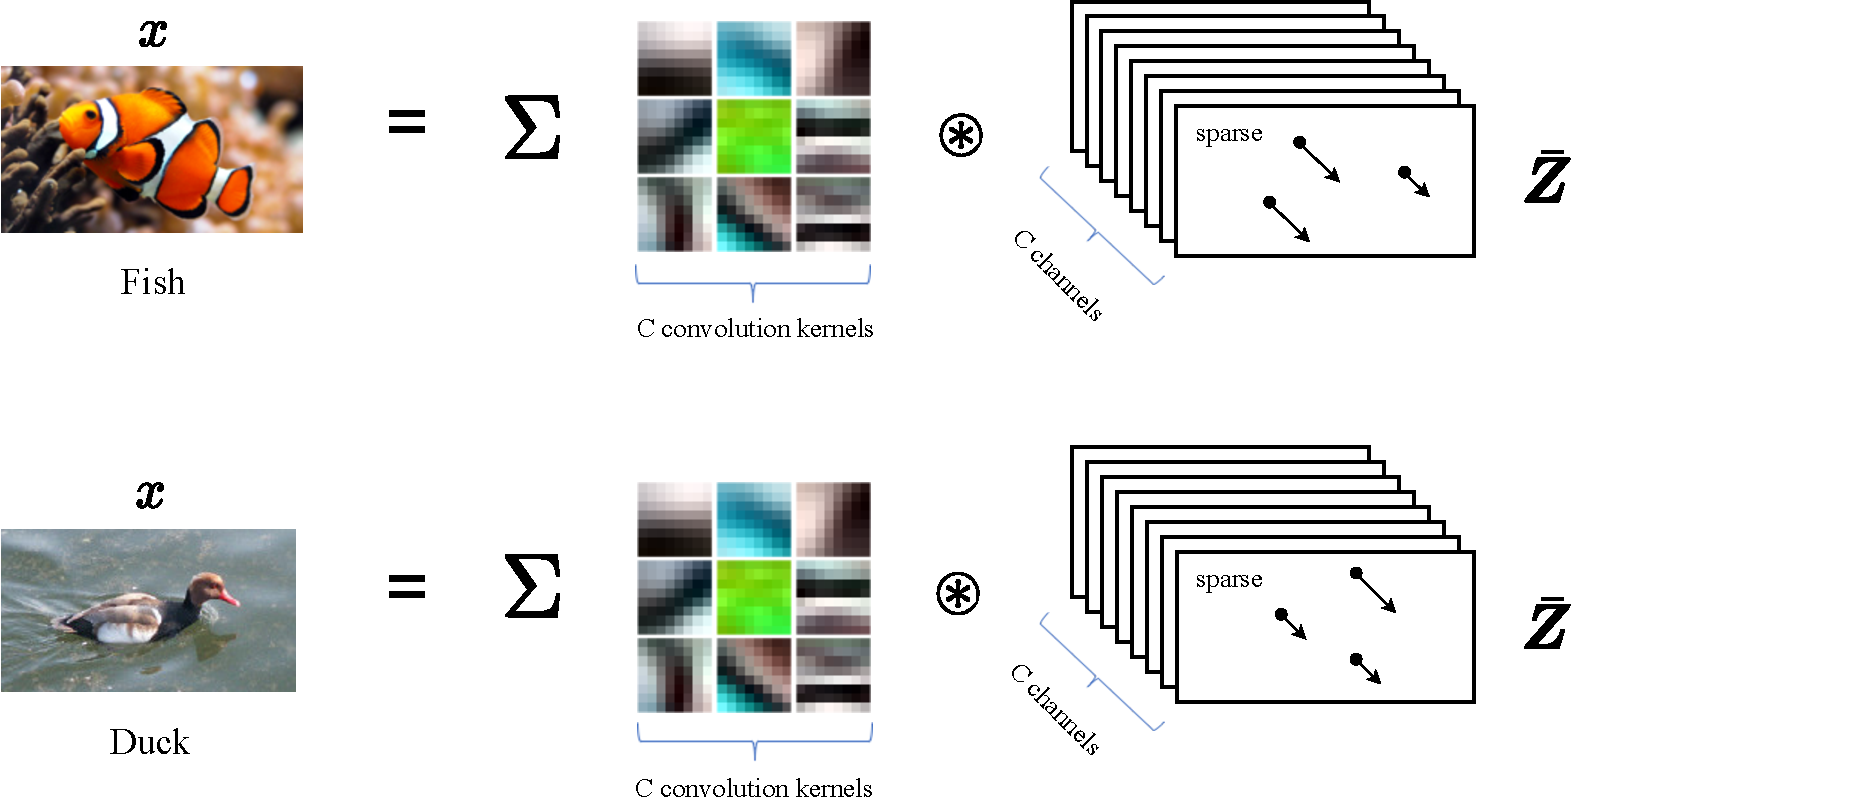
\includegraphics[width=0.9\textwidth]{\toplevelprefix/chapters/chapter4/figs/sparse-representation.pdf}}
	\caption{Each input signal $\bm x$ (an image here) can be represented as a superposition of sparse convolutions with multiple kernels $\bm d_c$ in a dictionary $\bm D$.}
	\label{fig:multi-channel-sparse-representation}
\end{figure}
One way of resolving this conflict is to leverage additional structure within each class, in the form of {\em sparsity}: signals within each class are not generated as an arbitrary linear superposition of some base atoms (or motifs), but only {\em sparse} combinations of them and their shifted versions, as shown in Figure \ref{fig:multi-channel-sparse-representation}. More precisely, let $\bm D_k = [\bm d_{k,1}, \ldots, \bm d_{k,c}]$ denote a matrix with a collection of atoms associated for class $k$, also known as a dictionary, then each signal $\x$ in this class is sparsely generated as: 
\begin{equation}
    \x = \bm d_{k,1} \circledast z_1 + \ldots + \bm d_{k,c} \circledast z_c = \circm(\bm{D}_k)\z,
\end{equation}
for some sparse vector $\z$. Signals in different classes are then generated by different dictionaries whose atoms (or motifs) are incoherent from one another. Due to incoherence, signals in one class are unlikely to be sparsely represented by atoms in any other class. Hence all signals can be represented as
\begin{equation}
\x = \big[\circm(\bm{D}_1), \circm(\bm{D}_2), \ldots, \circm(\bm{D}_K)\big] \bar \z,
\end{equation}
where $\bar \z$ is sparse.\footnote{Notice that similar sparse representation models have long been proposed and used for classification purposes in applications such a face recognition, demonstrating excellent effectiveness  \cite{Wright:2009,wagner2012toward}. Recently, the convolution sparse coding model has been proposed by \cite{papyan2017convolutional} as a framework for interpreting the structures of deep convolution networks.} There is a vast literature on how to learn the most compact and optimal sparsifying dictionaries from sample data, e.g.  \cite{li2019multichannel,qu2019nonconvex} and subsequently solve the inverse problem and compute the associated sparse code $\z$ or $\bar \z$. Recent studies of \cite{qu2020nonconvex,Qu2020Geometric} even show that under broad conditions the convolution dictionary learning problem can be solved effectively and efficiently. 

Nevertheless, for tasks such as classification, we are not necessarily interested in the precise optimal dictionary nor the precise sparse code for each individual signal. We are mainly interested if collectively the set of sparse codes for each class are adequately separable from those of other classes. Under the assumption of the sparse generative model, if the convolution kernels $\{\bm k_c\}_{c=1}^C$  match well with the ``transpose'' or ``inverse'' of the above sparsifying dictionaries $\bm D = [\bm D_1, \ldots, \bm D_K]$, also known as the {\em analysis filters} \cite{Cosparse-Nam,Analysis-Filter}, signals in one class will only have high responses to a small subset of those filters and low responses to others (due to the incoherence assumption).  Nevertheless, in practice, often a sufficiently large number of, say $C$, random filters $\{\bm k_c\}_{c=1}^C$ suffices to ensure that the extracted $C$-channel features
\begin{equation}
\big[\bm k_1 \circledast \x, \bm k_2 \circledast \x, \ldots, \bm k_C \circledast \x\big]^\top = \big[\circm(\bm k_1) \x, \ldots, \circm(\bm k_C) \x \big]^\top \in \Re^{C\times d}
\end{equation}
for different classes have different response patterns to different filters hence make different classes separable \cite{chan2015pcanet}. 

Therefore, in our framework, to a large extent the number of channels (or the width of the network) truly plays the role as the  {\em statistical resource} whereas the number of layers (the depth of the network) plays the role as the {\em computational resource}. The theory of compressive sensing precisely characterizes how many measurements are needed in order to preserve the intrinsic low-dimensional structures (including separability) of the data \cite{Wright-Ma-2021}. %

\begin{figure}[t]
	\centerline{
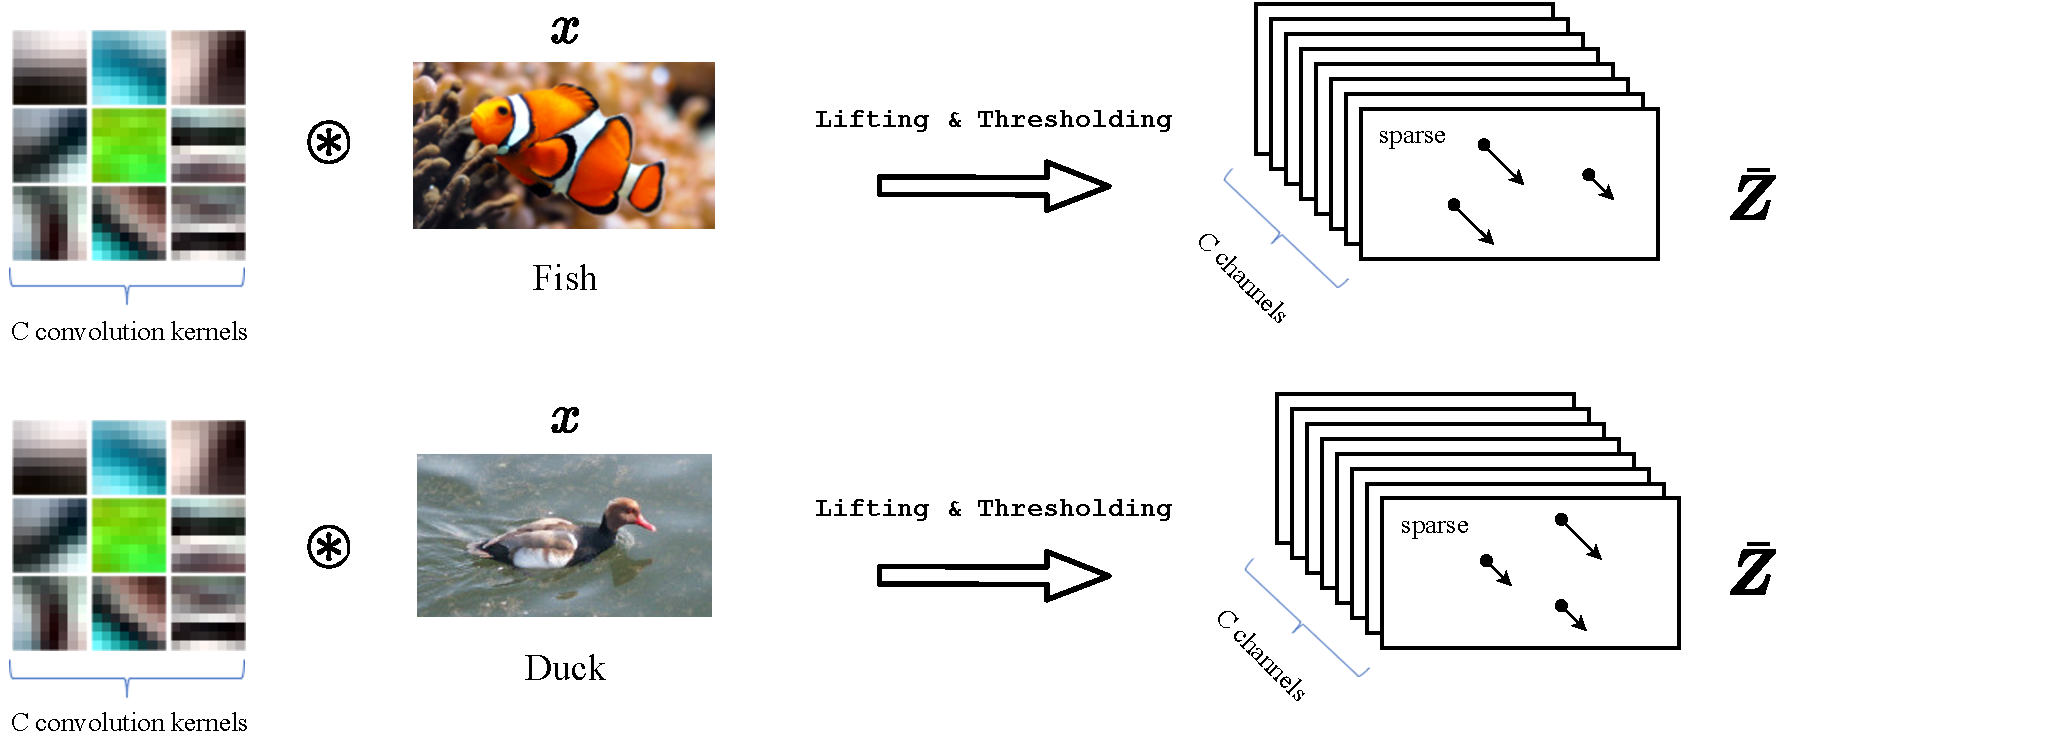
\includegraphics[width=0.95\textwidth]{\toplevelprefix/chapters/chapter4/figs/sparse-lifting.pdf}}
\caption{Estimate the sparse code $\bar{\bm z}$ of an input signal $\bm x$ (an image here) by taking convolutions with multiple kernels $\bm k_c$ and then sparsifying.}
		\label{fig:multi-channel-sparse-lifting}
\end{figure}
The multi-channel responses $\bar \z$ should be sparse. So to approximate the sparse code $\bar \z$, we may take an entry-wise {\em sparsity-promoting nonlinear thresholding}, say $\bm \tau(\cdot)$, on the above filter outputs by setting low (say absolute value below $\epsilon$) or negative  responses to be zero:
\begin{equation}
\bar \z \doteq \bm \tau \left( \big[\circm(\bm k_1) \x, \ldots, \circm(\bm k_C) \x \big]^\top \right) \in \Re^{C \times d}.
\label{eqn:sparse-lifting}
\end{equation} 
Figure \ref{fig:multi-channel-sparse-lifting} illustrates the basic ideas. One may refer to \cite{Analysis-Filter} for a more systematical study on the design of the sparsifying thresholding operator. Nevertheless, here we are not so interested in obtaining the best sparse codes as long as the codes are sufficiently separable. Hence the nonlinear operator $\bm \tau$ can be simply chosen to be a soft thresholding or a ReLU. 
These presumably sparse features $\bar \z$ can be assumed to lie on a lower-dimensional (nonlinear) submanifold of $\mathbb{R}^{dC}$, which can be linearized and separated from the other classes by subsequent ReduNet layers, as illustrated later in Figure \ref{fig:learn-to-classify-diagram}. 

The ReduNet constructed from circulant version of these multi-channel features $\bar\Z \doteq [\bar \z_1, \ldots, \bar \z_N] \in \Re^{C \times d \times N}$, i.e., $\circm(\bar\Z) \doteq [ \circm(\bar\z_1), \dots, \circm(\bar\z_N)] \in \Re^{dC \times dN}$, retains the good invariance properties described above: the linear operators, now denoted as $\bar{\bm E}$ and $\bar{\bm C}_k$, remain block circulant, and represent {\em multi-channel 1D circular convolutions. }
Specifically, we have the following result.
\begin{proposition}[Multi-channel convolution structures of $\bar{\bm E}$ and $\bar{\bm C}_k$]
The matrix 
\begin{equation}
\label{eq:def-E-bar}
\bar{\bm E} \doteq \alpha\left(\bm I + \alpha\, \circm(\bar\Z) \circm(\bar\Z)^\top \right) ^{-1}  
\end{equation}
is block circulant, i.e.,
\begin{equation*}
    \bar{\bm E} = 
    \left[\begin{matrix}
        \bar{\bm E}_{1, 1} & \cdots & \bar{\bm E}_{1, C}\\
        \vdots & \ddots & \vdots \\
        \bar{\bm E}_{C, 1} & \cdots & \bar{\bm E}_{C, C}\\
    \end{matrix}\right] \in \Re^{dC \times dC},
\end{equation*}
where each $\bar{\bm E}_{c, c'}\in \Re^{d \times d}$ is a circulant matrix. Moreover, $\bar{\bm E}$ represents a multi-channel circular convolution, i.e., for any multi-channel signal $\bar\z \in \Re^{C \times n}$ we have 
$$\bar{\bm E} \cdot \textsf{vec}(\bar\z) = \textsf{vec}( \bar{\bm e} \circledast \bar\z).$$ 
In above, $\bar{\bm e} \in \Re^{C \times C \times d}$ is a multi-channel convolutional kernel with $\bar{\bm e}[c, c'] \in \Re^{d}$ being the first column vector of $\bar{\bm E}_{c, c'}$, and $\bar{\bm e} \circledast \bar\z \in \Re^{C \times d}$ is the multi-channel circular convolution defined as
\begin{equation*}
    (\bar{\bm e} \circledast \bar\z)[c] \doteq \sum_{c'=1}^C \bar{\bm e}[c, c'] \circledast \bar{\z}[c'], \quad \forall c = 1, \ldots, C.
\end{equation*}
Similarly, the matrices $\bar{\bm C}_k$ associated with any subsets of $\bar{\bm Z}$ are also multi-channel circular convolutions. 
\label{prop:multichannel-circular-conv-1}
\end{proposition}
From Proposition \ref{prop:multichannel-circular-conv-1}, shift invariant ReduNet is a deep convolutional network for multi-channel 1D signals by construction. Notice that even if the initial lifting kernels are separated \eqref{eqn:sparse-lifting}, the matrix inverse  in \eqref{eq:def-E-bar} for computing $\bar{\bm E}$ (similarly for $\bar{\bm C_k}$) introduces ``cross talk'' among all $C$ channels. %
Hence, these multi-channel convolutions in general are {\em not} depth-wise separable, unlike the  Xception nets~\cite{Xception} that were once suggested to simplify multi-channel convolutional neural networks.\footnote{It remains open what additional structures on the data would lead to depth-wise separable convolutions.} 

\begin{remark}[Reducing Computational Complexity in the Frequency Domain] 
The calculation of $\bar{\bm E}$ in \eqref{eq:def-E-bar} requires inverting a matrix of size $dC \times dC$, which in general has complexity $O(d^3C^3)$.  Nevertheless, by using the fact that a circulant matrix can be diagonalized by the Discrete Fourier Transform (DFT) matrix, the complexity can be significantly reduced. As shown in \cite{chan2021redunet}, to compute $\bar{\bm E}$ and $\bar{\bm C}_k \in \Re^{dC \times dC}$, we only need to compute in the frequency domain the inverse of $C\times C$ blocks for $d$ times hence the overall complexity becomes $O(dC^3)$.
    
\end{remark}




\paragraph{Overall Network Architecture and Comparison.} 
Following the above derivation, we see that in order to find a linear discriminative representation (LDR)  for multiple classes of signals/images that is invariant to translation, sparse coding, a multi-layer architecture with multi-channel convolutions, different nonlinear activation, and spectrum computing all become {\em necessary} components for achieving the objective effectively and efficiently. Figure \ref{fig:learn-to-classify-diagram} illustrates the overall process of learning such a representation via invariant rate reduction on the input sparse codes. 

\begin{figure}[t]
    \centering
    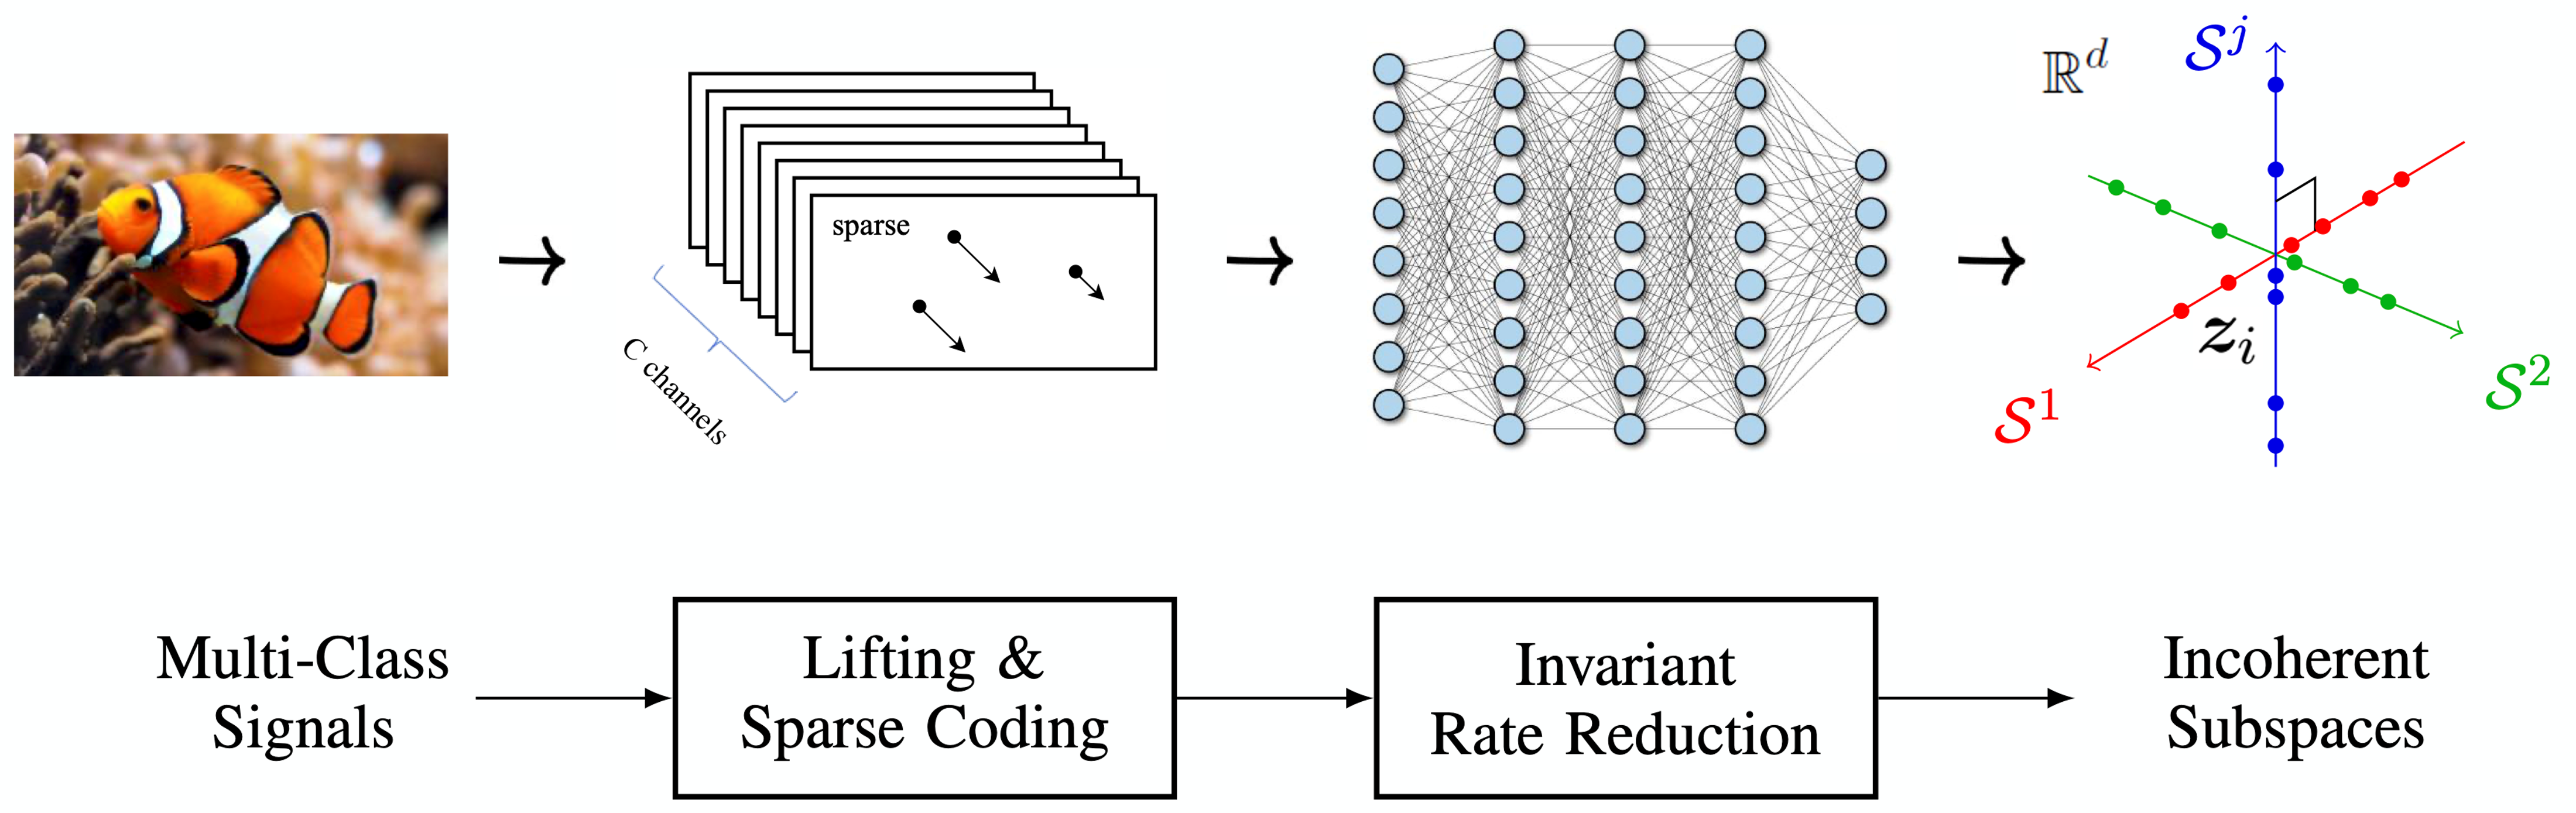
\includegraphics[width=0.98\linewidth]{\toplevelprefix/chapters/chapter4/figs/learn_to_classify_diagram_updated.png}
    \caption{The overall process for classifying multi-class signals with shift invariance: Multi-channel lifting,  sparse coding, followed by a multi-channel convolution ReduNet for invariant rate reduction. These components are {\em necessary} in order to map shift-invariant multi-class signals to incoherent (linear) subspaces as an LDR. Note that the architectures of most modern deep neural networks resemble this process. The so-learned LDR facilitates subsequent tasks such as classification.}
    \label{fig:learn-to-classify-diagram}
\end{figure}


\begin{example}[Invariant Classification of Digits]
We next provide an empirical performance of the ReduNet on learning \textit{rotation} invariant features on the real 10-class MNIST dataset. 
We impose a polar grid on the image $\bm{x}\in\mathbb{R}^{H\times W}$, with its geometric center being the center of the 2D polar grid (as illustrated in Figure \ref{fig:samples-invariant-1d-mnist-diagram}). 
For each radius $r_i$, $i \in [C]$, we can sample $\Gamma$ pixels with respect to each angle $\gamma_l =l\cdot({2\pi}/\Gamma)$ with $l \in [\Gamma]$. 
Then given a sample image $\bm{x}$ from the dataset, we represent the image in the (sampled) polar coordinate as a multi-channel signal $\bm{x}_p \in\R^{\Gamma\times C}$.  
The goal here is to learn a rotation invariant representation, i.e., we expect to learn $f(\cdot, \bm{\theta})$ such that $\{f(\bm{x}_p \circ \mathfrak{g}, \bm{\theta})\}_{\mathfrak{g} \in\mathbb{G}}$ lie in the same subspace, where $\mathfrak{g}$ is the cyclic-shift in polar angle.  
We use $N=100$ training samples ($10$ from each class) and set $\Gamma=200$, $C=15$ for polar sampling. 
By performing the above sampling in polar coordinate, we can obtain the data matrix $\bm{X}_p \in \mathbb{R}^{(\Gamma\cdot C) \times N}$. 
For the ReduNet, we set the number of layers/iterations $L=40$, precision $\epsilon=0.1$, step size $\eta=0.5$. Before the first layer, we perform lifting of the input by 1D circulant-convolution with 20 random Gaussian kernels of size 5.   

\begin{figure}[t]
    \begin{subfigure}[t]{0.3\textwidth}
        \centering
        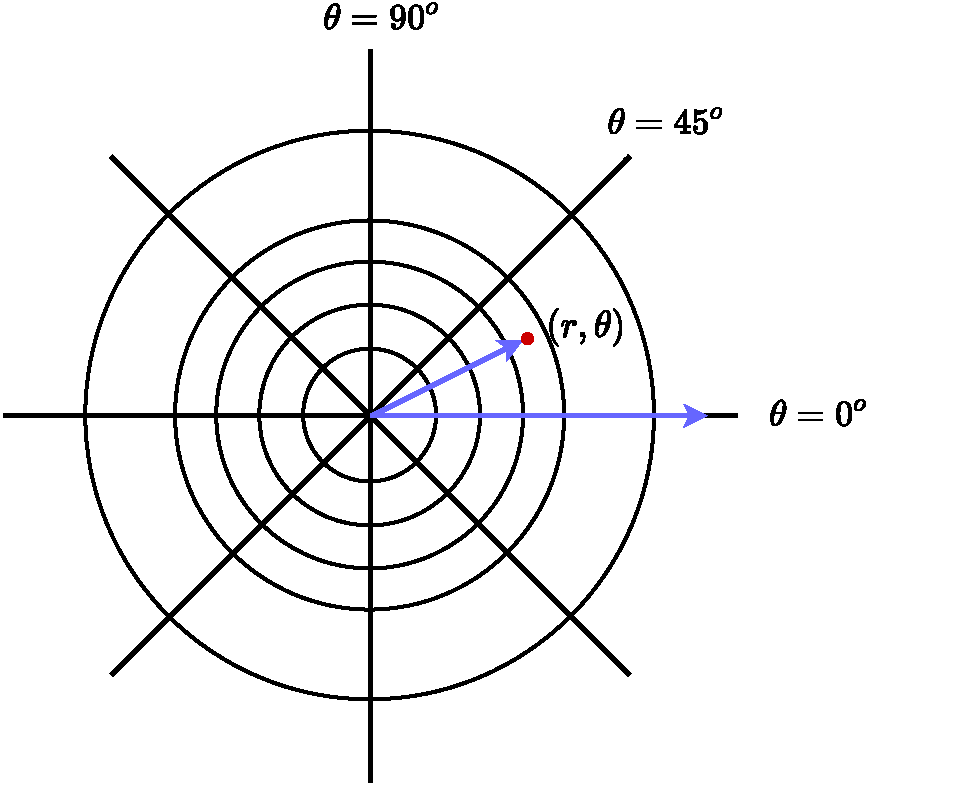
\includegraphics[width=\textwidth]{\toplevelprefix/chapters/chapter4/figs/1d-rotation.pdf}
        \caption{$\bm{X}_{\text{rotation}}$}
    \end{subfigure}
    \hfill
    \begin{subfigure}[t]{0.3\textwidth}
        \centering
        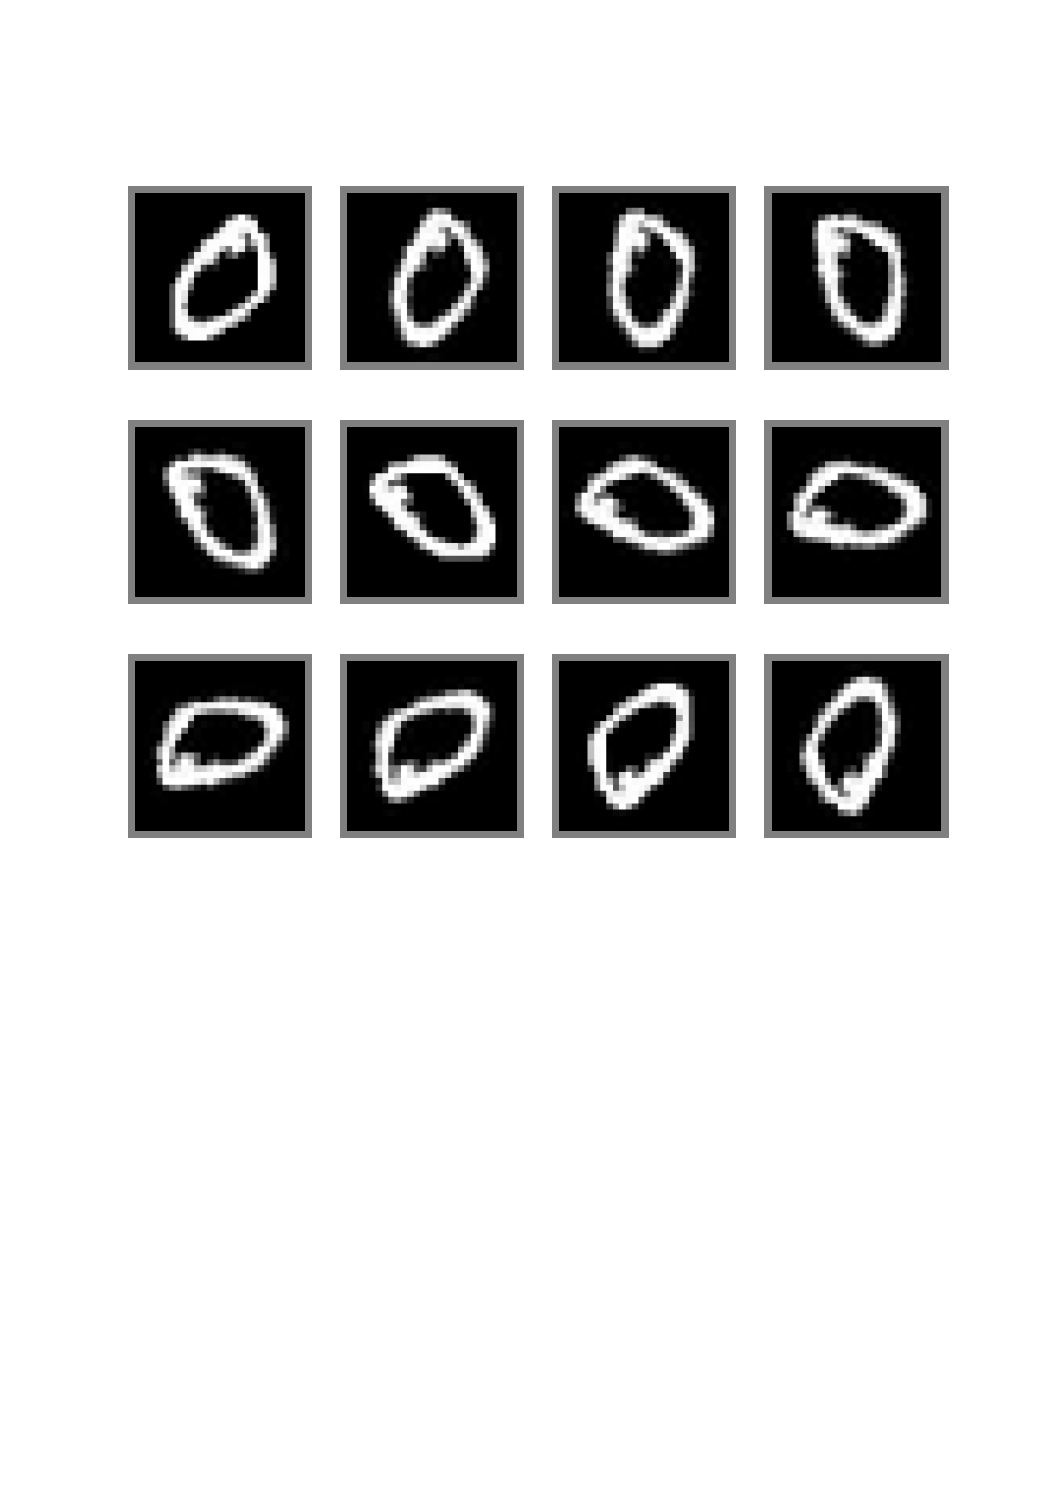
\includegraphics[width=\textwidth]{\toplevelprefix/chapters/chapter4/figs/mnist1d_img0.pdf}
        \caption{$\bm{Z}_{\text{rotation}}$}
    \end{subfigure}
    \hfill
    \begin{subfigure}[t]{0.3\textwidth}
        \centering
        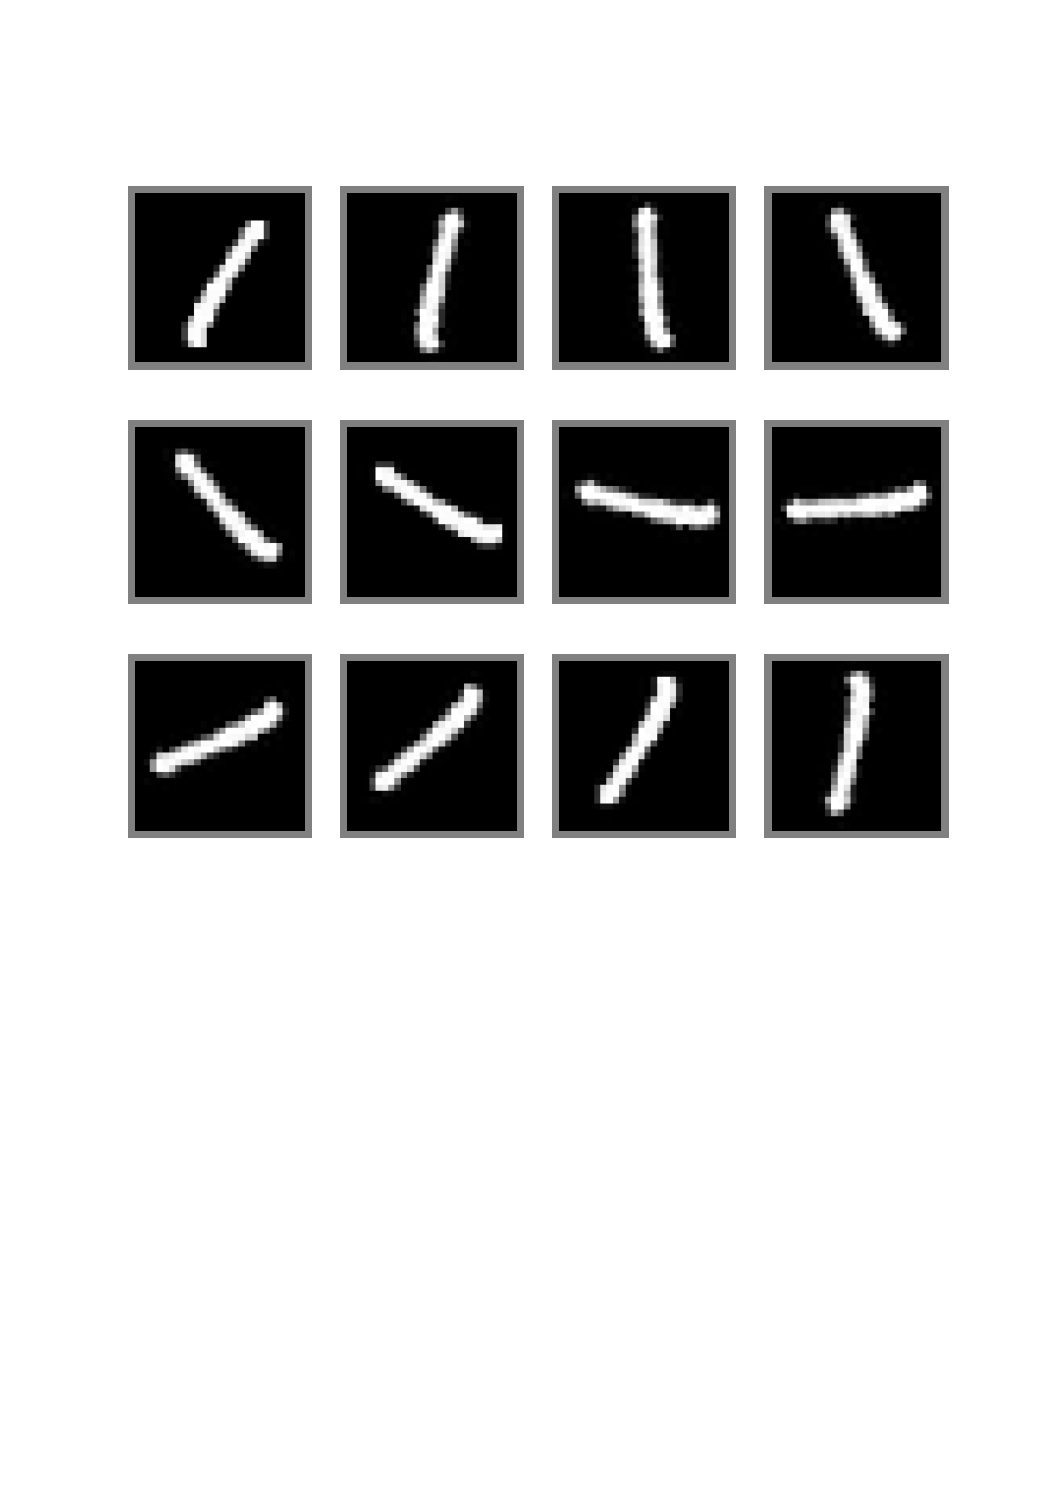
\includegraphics[width=\textwidth]{\toplevelprefix/chapters/chapter4/figs/mnist1d_img1.pdf}
        \caption{Loss}
    \end{subfigure}
    \caption{\small Examples of rotated images of MNIST digits, each by 18$^{\circ}$. (\textbf{Left}) Diagram for polar coordinate representation;  (\textbf{Right}) Rotated images of digit `0' and `1'.}
    \label{fig:samples-invariant-1d-mnist-diagram}
\end{figure}


To evaluate the learned representation, each training sample is augmented by 20 of its rotated version, each shifted with stride=10. We compute the cosine similarities among the $m \times 20$ augmented training inputs $\bm{X}_{\text{rotation}}$ and the results are shown in Figure~\ref{fig:redu-invariant-1d-mnist-diagram} (\textbf{a}). 
We compare the cosine similarities among the learned features of all the augmented versions, i.e., $\bar{\bm{Z}}_{\text{rotation}}$ and summarize the results in  Figure~\ref{fig:redu-invariant-1d-mnist-diagram} (\textbf{b}). 
As we see, the so constructed rotation-invariant ReduNet is able to  map the training data (as well as all its rotated versions) from the 10 different classes into 10 nearly orthogonal subspaces. That is, the learnt subspaces are truly invariant to shift transformation in polar angle.  Next, we randomly draw another $100$ test samples followed by the same augmentation procedure. 
In Figure~\ref{fig:redu-invariant-1d-mnist-diagram} (\textbf{c}), we visualize the MCR$^{2}$ loss on the  $\ell$-th layer representation of the ReduNet on the training and test dataset. From these results, we can find that the constructed ReduNet is indeed able to maximize the MCR$^{2}$ loss as well as generalize to the test data.



\begin{figure}[t]
    \begin{subfigure}[t]{0.3\textwidth}
        \centering
        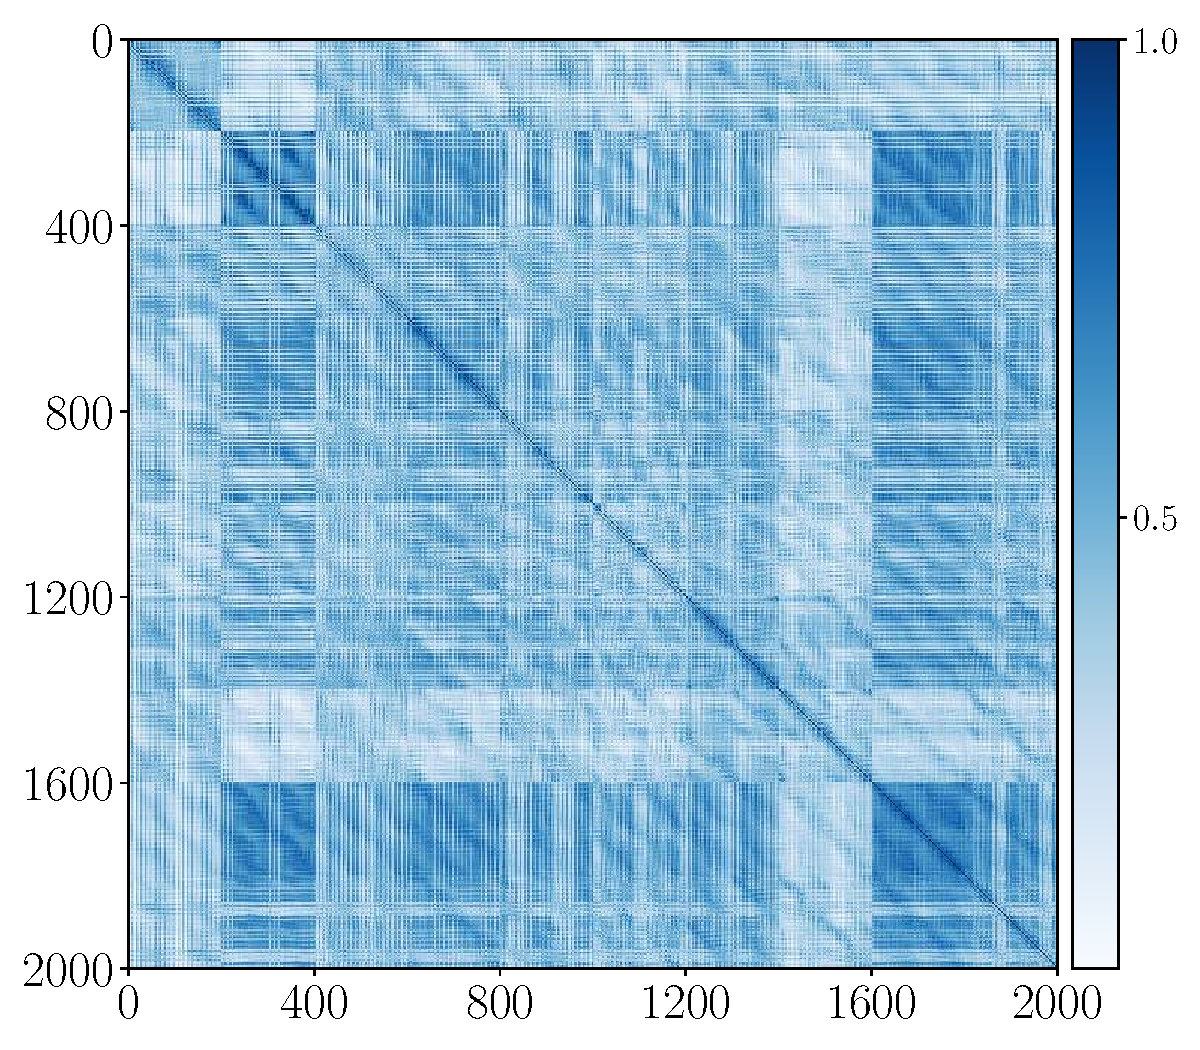
\includegraphics[width=\textwidth]{\toplevelprefix/chapters/chapter4/figs/mnist1d-heatmap-X_translate_train_all.pdf}
        \caption{$\bm{X}_{\text{rotation}}$}
    \end{subfigure}
    \hfill
    \begin{subfigure}[t]{0.3\textwidth}
        \centering
        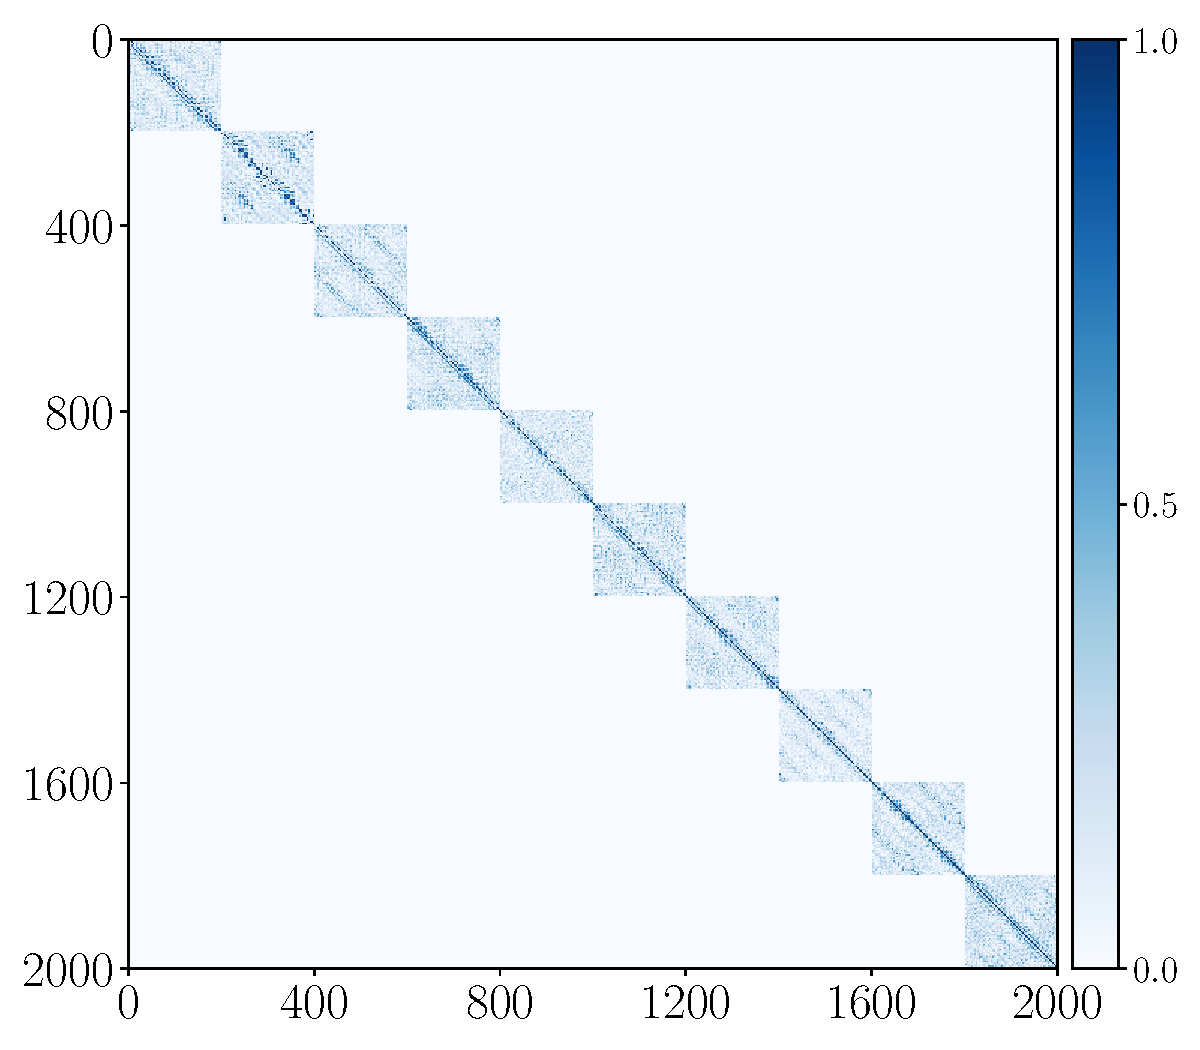
\includegraphics[width=\textwidth]{\toplevelprefix/chapters/chapter4/figs/mnist1d-heatmap-Z_translate_train_all.pdf}
        \caption{$\bm{Z}_{\text{rotation}}$}
    \end{subfigure}
    \hfill
    \begin{subfigure}[t]{0.32\textwidth}
        \centering
        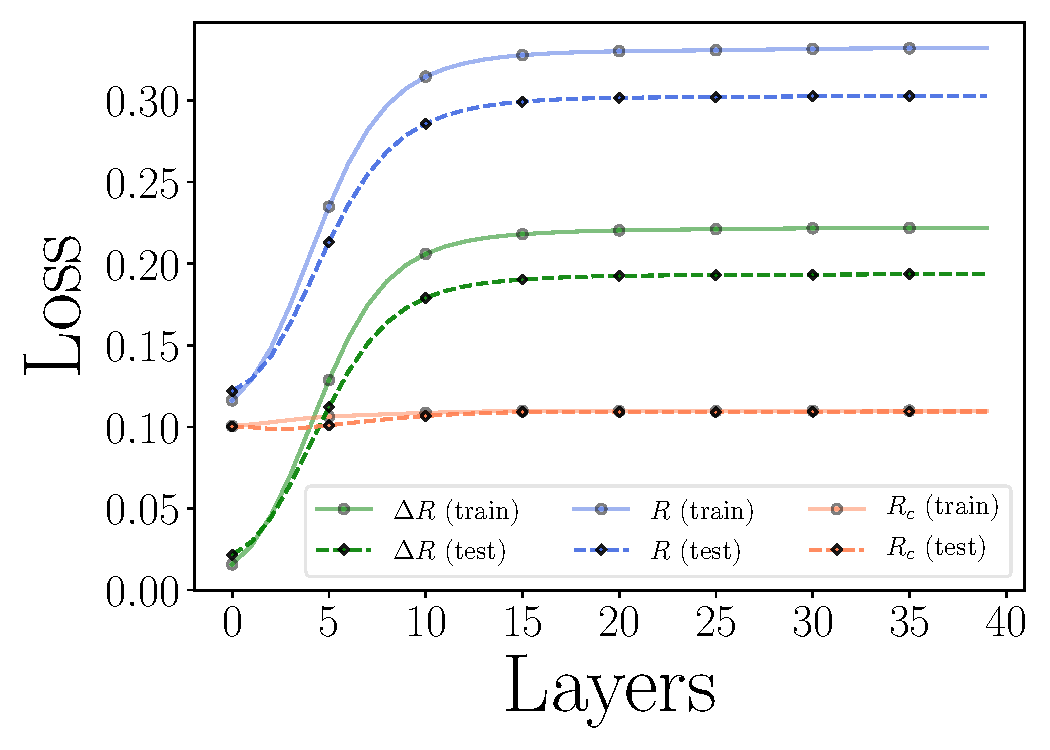
\includegraphics[width=\textwidth]{\toplevelprefix/chapters/chapter4/figs/mnist1d-loss-traintest.pdf}
        \caption{Loss}
    \end{subfigure}
    \caption{\small (a)(b) are heatmaps of cosine similarity among rotated training data $\bm{X}_{\text{rotation}}$ and learned features $\bar{\bm{Z}}_{\text{rotation}}$ for rotation invariance. (d) visualizes the training/val MCR$^2$ losses across layers.}
    \label{fig:redu-invariant-1d-mnist-diagram}
\end{figure}

\end{example}
















 




\section{White-Box Transformers from Unrolled Optimization}\label{sec:chap4-white-box-transformer}
As we have seen in the previous section, we use the problem of classification to provide a rigorous interpretation for main architectural characteristics of popular deep networks such as the ResNet and the CNN: each layer of such networks can be viewed as to imitate a gradient step which increases the rate reduction (or information gain) objective. This perspective also leads to a somewhat surprising fact: the the parameters and operators  of the layers of such a deep network, the ReduNet, can be  computed in a purely forward fashion.

Despite the theoretical and conceptual importance of the ReduNet, several factors limit it from being very practical. First, as we have discussed in the above, the computational cost of computing the matrix operators in  each layer in a forward fashion can be very high. Second, the so-computed operators may not be so effective in optimizing the objective and it might take thousands of iterations (hence layers). As we have seen  in \Cref{sec:LISTA} for LISTA, these two issues can be addressed by allowing to optimize those operators and make them learnable via back-propagation.\footnote{Or, perhaps, by a mixture of both forward and backward optimization.}

The supervised classification setting in which the ReduNet was derived is also somewhat limiting. In practice, an image might not belong to a single class as it may contain multiple objects. Hence it would be more general to assume that different regions of the image belong to  different low-dimensional models (say a Gaussian or a subspace). As we will see, such a generalization would lead to a both simple and general architecture which unifies the rate reduction and the denoising operations that we have seen in the previous chapter. Moreover, the so-obtained architecture resembles the popular Transformer architecture.



\subsection{Unrolled Optimization for Sparse Rate Reduction}



We consider a general learning setup associated with real-world signals. Let \(\X = \mat{\x_{1}, \dots, \x_{N}} \in \bR^{D \times N}\) denote random variables representing our data source. In vision tasks, each \(\x_{i} \in \bR^{D}\) is interpreted as a \textit{token}, typically corresponding to an image patch. In language tasks, each \(\x_{i} \in \bR^{D}\) is interpreted as an \textit{token embedding}, i.e., a continuous vector representation of a discrete token such as a word or subword.\footnote{With a slight abuse of terminology, we refer to both the discrete tokens and their associated embeddings simply as tokens throughout this chapter for convenience.}  %
The \(\x_{i}\)'s may have arbitrary correlation structures. We use \(\Z = \mat{\z_{1}, \dots, \z_{N}} \in \bR^{d \times N}\) to denote the random variables that defines our representations, where \(\z_{i} \in \bR^{d}\) is the representation of the corresponding token \(\x_i \in \bR^{D}\).%

\begin{remark}
    In transformers, each input sample is typically converted into a sequence of {\em tokens}. A token is a basic unit of information derived from the raw input: in natural language processing, tokens are typically words or subwords; in computer vision, they correspond to image patches; and in other modalities, they may represent time steps, spatial locations, or other domain-specific units. A {\em token embedding} is a continuous vector representation of a token that serves as the input to a transformer. It maps each token to a point in a high-dimensional space, enabling the model to process symbolic inputs using numerical computation.
    A {\em token representation} is a vector that encodes the semantic or structural information of a token, typically produced by the intermediate or final layers of a transformer. These representations are designed to capture meaningful features of the input that are useful for downstream tasks such as classification, generation, or regression. Please refer to \Cref{sec:contrastive_learning} for more details about these concepts in implementations. 
\end{remark}


 
\paragraph{Objective for Learning a Structured and Compact Representation.}
Following the framework of rate reduction \Cref{sec:chap4-white-box-model-via-unrolling}, we contend
that the goal of representation learning is to find a feature mapping \(f
\colon \X \in \bR^{D \times N} \to \Z\in \bR^{d \times N}\) which transforms input tokens \(\{\bm x_i\}_{i=1}^N \subset \R^D\) with a potentially nonlinear and multi-modal distribution to a (piecewise) \textit{linearized and compact} token representations \(\{\bm z_i\}_{i=1}^N \subset \bR^{d}\). While the joint distribution of tokens representations \(\{\z_{i}\}_{i = 1}^{N}\) may be sophisticated (and task-specific), we further contend that it is reasonable and practical to
require that the target marginal distribution of individual token representations should be highly compressed and structured, amenable for compact coding. Particularly, we require the distribution to be \textit{a mixture of low-dimensional (say \(K\)) Gaussian
distributions}, such that the \(k\)-th Gaussian has mean \(\Zero \in \bR^{d}\), covariance \(\vSigma_{k} \succeq \Zero \in \bR^{d \times d}\), and support spanned by the orthonormal basis \(\vU_{k} \in \bR^{d \times p}\). 
We denote $\vU_{[K]} = \{\vU_k\}_{k=1}^K$ to be the set of bases of all Gaussians. Hence, to maximize the \textit{information gain} \cite{ma2022principles} for the final token representations, we wish to maximize their rate reduction (see \Cref{subsec:MCR2}), i.e., 
\begin{align}\label{eq:rate reduction}
    \mathrm{max}_{\bm Z \in \R^{d\times N}}\ \Delta R_{\epsilon}(\Z \mid \vU_{[K]}) \doteq R_{\epsilon}(\Z) - R^c_{\epsilon}(\Z \mid \vU_{[K]}).
\end{align}
Here, the first term $R_{\epsilon}$ is an estimate of the lossy coding rate for the whole set of token representations. More specifically, if we view the token representations $\{\bm z_i\}_{i=1}^N$ as i.i.d. samples from a single zero-mean Gaussian, their lossy coding rate subject to a quantization precision $\epsilon > 0$ is given as
\begin{equation}\label{eq:coding_rate}
    R_{\epsilon}(\Z) \doteq \frac{1}{2}\textrm{logdet}\left(\I + \frac{d}{N\epsilon^{2}}\Z^{\top}\Z\right) = \frac{1}{2}\textrm{logdet}\left(\I + \frac{d}{N\epsilon^{2}}\Z\Z^{\top}\right).
\end{equation}
The second term $R_{\epsilon}^c$ is an estimate of the lossy coding rate under the codebook $\bm U_{[K]}$, which is given as 
\begin{equation}
\begin{aligned}
    R_{\epsilon}^c(\Z \mid \vU_{[K]}) &\doteq \sum_{k=1}^{K}R_{\epsilon}(\vU_k^{\top} \Z) = \frac{1}{2}\sum_{k=1}^{K}\log\det\left(\I +
    \frac{p}{N\epsilon^{2}}(\vU_k^{\top}\Z)^{\top}(\vU_k^{\top}\Z)\right).
\end{aligned}
\label{eq:def-mcr-Rc}
\end{equation}

\begin{remark}
    The expression \eqref{eq:def-mcr-Rc} for the coding rate can be viewed as a generalization of the coding rate \(R_\epsilon^{c}\) used in the original rate reduction objective \eqref{eq:MCRc}. In particular, the original objective is defined with respect to a set of known membership labels \(\{\vPi_{k}\}\) specific to the particular data realization \(\vX\). In contrast, the current objective is defined with respect to subspaces \(\vU_{[K]}\), which are independent of any particular realization but are assumed to support the distribution of token representations. Suppose that a token representation $\bm z_i$ belongs to a subspace $\bm U_k$ and these subspaces are approximately orthogonal to each other, i.e., $\bm U_k^\top \bm U_l \approx \bm 0$ for all $k \neq l$. Then, one can verify that the projections $\bm U_k\bm U_k^\top \bm z_i  = \bm z_i$ and  $\bm U_l\bm U_l^\top \bm z_i \approx \bm 0$ for all $l \neq k$. These orthogonal projections effectively serve as implicit membership labels, identifying the subspace to which each token representation belongs. 
\end{remark}



\begin{figure}[t!]
     \centering
         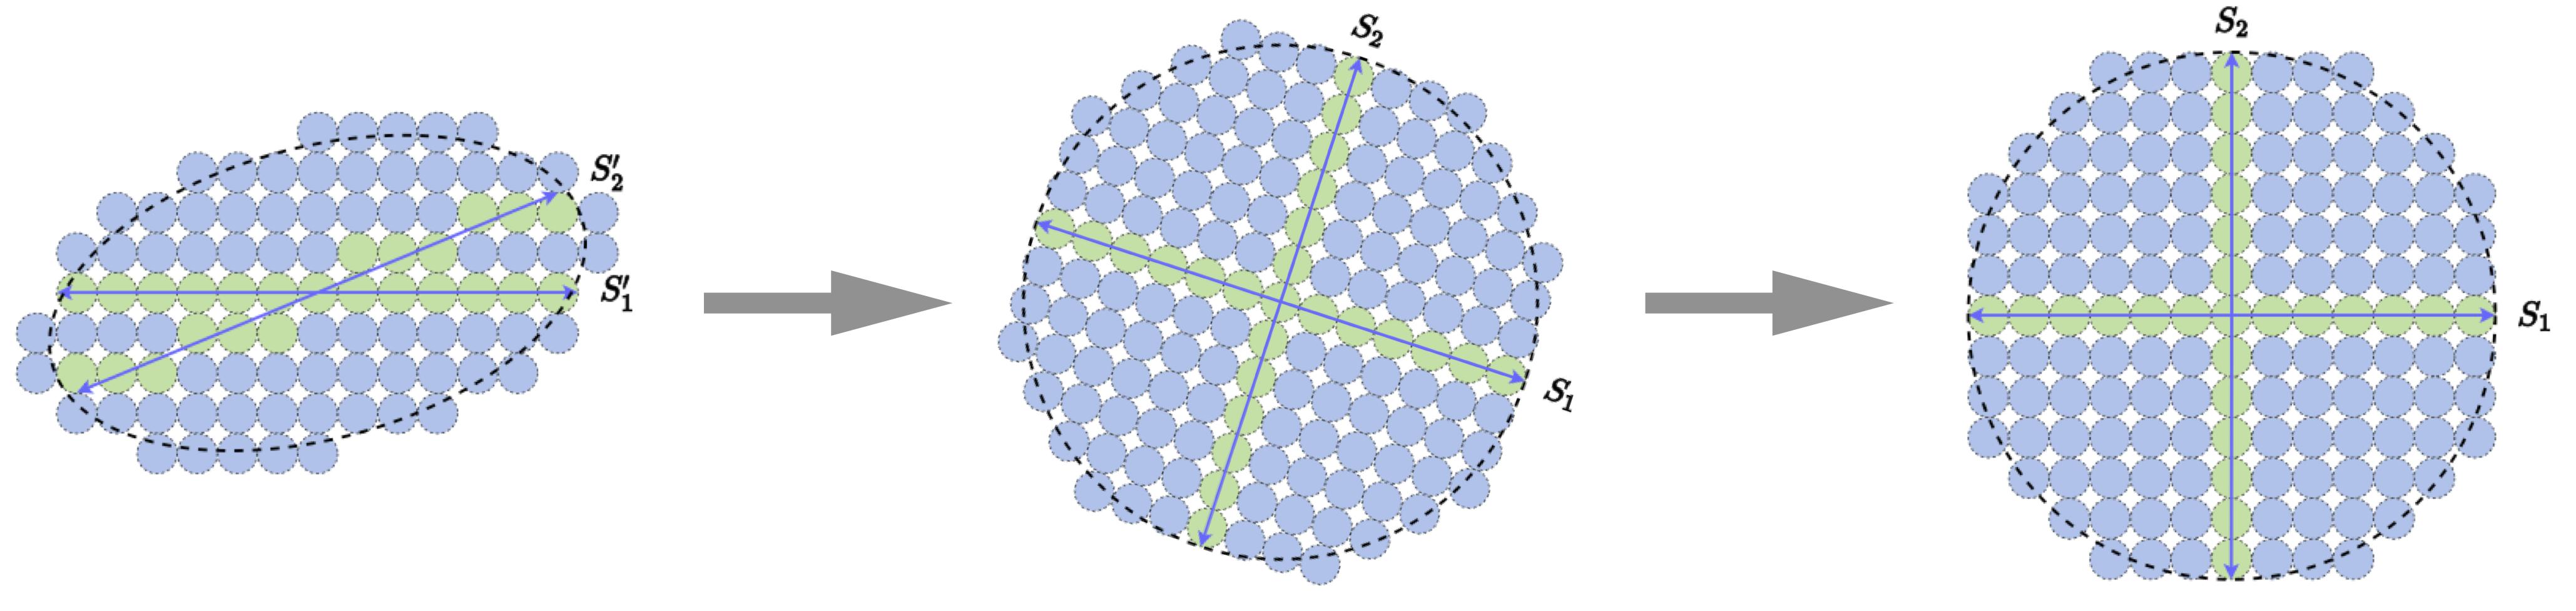
\includegraphics[width=0.95\textwidth]{\toplevelprefix/chapters/chapter4/figs/coding-transform.png}
     \caption{ \small\textbf{Comparison of three sets of  representations via rate reduction and sparsity.} Each $S_i$ represents one linear subspace, and the number of blue balls represents the difference between the coding rates $\Delta R_{\epsilon}(\vZ \mid \vU_{[K]}) = R_\epsilon(\vZ) - R^c_\epsilon(\vZ \mid \vU_{[K]})$. 
     }
        \label{fig:sparse-rate-reduction-diagram}
\end{figure}


\paragraph{Sparse Rate Reduction.} Note that the rate reduction objective \eqref{eq:rate reduction} is invariant to arbitrary joint rotations of the representations and subspaces. In particular, optimizing the rate reduction objective may not naturally lead to axis-aligned (i.e., \textit{sparse}) representations. {For instance, consider the three sets of learned representations in \Cref{fig:sparse-rate-reduction-diagram}. The coding rate reduction increases from (a) to (b), but because it is invariant under rotations, remains the same from (b) to (c).} Therefore, we would like to transform the representations (and their supporting subspaces) so that the representations $\vZ$ eventually become sparse\footnote{Concretely, having few nonzero entries.} with respect to the standard coordinates of the resulting representation space {as in \Cref{fig:sparse-rate-reduction-diagram}(c)}. Therefore, to ensure the final representations are amenable to more compact coding, we would like to transform the representations (and their supporting subspaces) so that they become \textit{sparse} with respect to the standard coordinates of the resulting representation space.\footnote{That is, having the fewest nonzero entries.} Computationally, we may combine the above two goals into a unified objective for optimization:
\begin{equation}
   \max_{f \in \mathcal{F}}\ [\Delta R_{\epsilon}(\Z \mid \vU_{[K]}) - \lambda \|\bm{Z}\|_0] \qquad \text{s.t.}\ \Z = f(\X),
   \label{eq:sparse-rr}
\end{equation}
where $\mathcal{F}$ denotes a general function class and the $\ell_0$ norm $\|\Z\|_0$ promotes the sparsity of the final token representations \(\Z = f(\X)\).%


In practice, the $\ell_0$ norm is often relaxed to the $\ell_1$ norm to improve computational traceability and enable convex optimization techniques \cite{Wright-Ma-2022}. Motivated by this, we relax Problem \eqref{eq:sparse-rr} accordingly, leading to a formulation that remains faithful to the original sparsity objective while being more amenable to efficient algorithms as follow:  
\begin{equation}
\begin{aligned}
   \max_{f \in \mathcal{F}}\ [\Delta R_{\epsilon}(\Z \mid \vU_{[K]}) - \lambda \|\bm{Z}\|_1]  \qquad \text{s.t.}\ \Z = f(\X),
   \label{eq:sparse-rr-1}
\end{aligned}
\end{equation}
 With a slight abuse of terminology, we often refer to this objective function also as the \textit{sparse rate reduction}. 

\paragraph{White-Box Network Architecture via Unrolled Optimization.} 


Although easy to state, each term in the above objective is computationally challenging to optimize \cite{Wright-Ma-2022}. Hence it is natural to adopt an approximation approach that realizes the global transformation $f$ to optimize 
\eqref{eq:sparse-rr} through a concatenation of multiple, say $L$, simple \textit{incremental and local} operations $f^\ell$ that push the representation distribution towards the desired parsimonious model distribution:
\begin{equation}
f\colon \X = \bm Z^0 \xrightarrow{\hspace{1mm} f^0 \hspace{1mm}} \Z^1 \rightarrow \cdots \rightarrow \Z^\ell \xrightarrow{\hspace{1mm} f^{\ell} \hspace{1mm}} \Z^{\ell+1} \rightarrow  \cdots \xrightarrow{\hspace{1mm} f^{L-1}} \Z^L = \Z,
\label{eq:incremental}
\end{equation}
where $f^0: \bR^{D} \rightarrow \bR^{d}$ is the pre-processing mapping that transforms each input token $\x_{i} \in \bR^{D}$ to the initial token representations $\z_{i}^{1} \in \bR^{d}$.  
Each incremental \textit{forward mapping} $\Z^{\ell + 1} = f^\ell(\Z^\ell)$, or a ``layer'', transforms the token distribution to \textit{optimize} the above sparse rate reduction objective \eqref{eq:sparse-rr}, conditioned on the distribution of its input $\Z^\ell$. 

\begin{remark}
    In contrast to other unrolled optimization approaches such as the ReduNet (see \Cref{sec:chap4-white-box-model-via-unrolling}), we \textit{explicitly model} the distribution of $\Z^\ell$ at each layer, say as a mixture of linear subspaces or sparsely generated from a dictionary. The model parameters are learned from data (say via \textit{backward propagation} with end-to-end training). This separation between forward ``optimization'' and backward
``learning'' clarifies the mathematical role of each layer as an operator
that transforms the distribution of its input, whereas the input distribution is in turn modeled (and subsequently learned) by the parameters of the layer. 
\end{remark}

Now, we show how to derive these incremental and local operations through an unrolled optimization perspective to solve Problem \eqref{eq:sparse-rr-1}.  Once we decide on using an incremental approach to optimizing Problem
\eqref{eq:sparse-rr-1}, there are a variety of possible choices to achieve the optimization. Given a model for $\Z^\ell$, say a mixture of subspaces $\vU_{[K]}$, we opt for a two-step \textit{alternating minimization} method with a strong conceptual basis. First, we \textit{compress} the tokens $\vZ^{\ell}$ via a gradient descent to minimize the coding rate term $R^c_\epsilon (\vZ \mid \vU_{[K]}^\ell)$. Specifically, we take a gradient step on $R^c_\epsilon$ with a learning rate $\kappa$ as follows:
\begin{align}\label{eq:Z l+1/2}
    \bm Z^{\ell+1/2} = \bm Z^\ell - \kappa \nabla_{\bm Z} R^c_\epsilon (\vZ \mid \vU_{[K]}^\ell). 
\end{align}
Next, we \textit{sparsify} the compressed tokens, generating \(\vZ^{\ell + 1}\) via a suitably-relaxed proximal gradient step to minimize the remaining term $\lambda \norm{\vZ}_{1} - R_{\epsilon}(\vZ)$. As we will argue in detail later, we can find such a $\bm Z^{\ell+1}$ by solving a sparse presentation problem with respect to a dictionary $\bm D^\ell$:
\begin{equation}\label{eq:Z l+1}
  \vZ^{\ell+1} = \argmin_{{\vZ}}  \bigg\{\lambda \norm{\vZ}_1 + \frac{1}{2}\norm{\vZ^{\ell + 1/2} - \vD^{\ell} {\vZ}}_F^2\bigg\}.
\end{equation}
In the following, we provide technical details for each of the two steps above and derive efficient updates for their implementation.




\paragraph{Self-Attention as Gradient Descent on Coding Rate of Token Representations.} For the first step \eqref{eq:Z l+1/2}, the gradient of the coding rate \(\nabla_{\bm Z} R^c_\epsilon\) is costly to compute, as it involves \(K\) separate matrix inverses, one for each of the \(K\) subspaces with basis \(\vU_{k}^{\ell}\):
\begin{equation}
    \nabla_{\bm Z} R_{\epsilon}^c(\vZ \mid \vU_{[K]})
    = \frac{p}{N\epsilon^2}\sum_{k=1}^K \vU_k\vU_k^\top\vZ\Big(\I +
    \frac{p}{N\epsilon^2}(\vU_k^\top\vZ)^\top(\vU_k^\top\vZ)\Big)^{-1}.
    \label{eq:rate-gradient}
\end{equation}
Now, we demonstrate that this gradient can be naturally approximated using a so-called multi-head subspace self-attention (MSSA) operator, which has a similar functional form to the multi-head self-attention operator \citep{vaswani2017attention} with \(K\) heads (i.e., one for each subspace, coming from each matrix inverse). Here, we approximate the gradient \eqref{eq:rate-gradient} using the first-order Neumann series (see \Cref{ex:neumannn}):
\begin{align}\label{eq:gd_rc_neumann}
    \nabla_{\bm Z} R_{\epsilon}^{c}(\vZ \mid \vU_{[K]}) 
    &\approx \frac{p}{N\epsilon^2} \sum_{k = 1}^{K}\vU_{k}\vU_{k}^\top\vZ\left(\vI - \frac{p}{N\epsilon^2} (\vU_{k}^\top\vZ)^\top(\vU_{k}^\top\vZ)\right) \notag \\
    &{= \frac{p}{N\epsilon^2} \left(\sum_{k = 1}^{K} \vU_{k}\vU_{k}^\top\right)\vZ -  \left( \frac{p}{N\epsilon^2}\right)^2\sum_{k = 1}^{K} \vU_{k}(\vU_{k}^\top\vZ)(\vU_{k}^\top\vZ)^\top(\vU_{k}^\top\vZ)}.
\end{align}
In this approximation, we compute the similarity between projected token representations $\{\bm U_k^\top\bm z_i\}$ through an auto-correlation among the projected features as $(\vU_{k}^\top\vZ)^\top(\vU_{k}^\top\vZ)$ and convert it to a distribution of membership with a softmax, namely $\softmax{(\vU_{k}^\top\vZ)^\top(\vU_{k}^\top\vZ)}$. 
Suppose that a union of subspaces $\bm U_{[K]}$ spans the whole space. Then, we have $\sum_{k = 1}^{K} \vU_{k}\vU_{k}^\top = \bm I$. Hence, \eqref{eq:gd_rc_neumann} becomes
\begin{align}\label{eq:grad Rc}
    \nabla_{\bm Z} R_{\epsilon}^{c}(\vZ \mid \vU_{[K]}) 
     \approx  \frac{p}{N\epsilon^2} \vZ -  \left( \frac{p}{N\epsilon^2}\right)^2 \MSSA\left(\vZ^{\ell} \mid \vU_{[K]}^{\ell}\right),
\end{align}
where MSSA is defined through an SSA operator as follows:
\begin{align}
    & \mathrm{SSA}\left(\vZ \mid \vU_{k}\right) 
    \doteq (\vU_{k}^\top \vZ)\mathrm{softmax}\left((\vU_{k}^\top\vZ)^\top(\vU_{k}^\top\vZ)\right), \ \forall k \in [K], \label{eq:SSA} \\
    & \mathrm{MSSA}\left(\vZ \mid \vU_{[K]}\right) 
    \doteq \frac{p}{N\epsilon^2} \mat{\vU_{1}, \dots, \vU_{K}}\mat{\mathrm{SSA}({\vZ \mid \vU_{1}}) \\ \vdots \\ \mathrm{SSA}({\vZ \mid \vU_{K}})}.\label{eq:Multi-Head-SSA}
\end{align}  
Substituting \eqref{eq:grad Rc} into \eqref{eq:Z l+1/2} yields that it can naturally approximated by
\begin{equation}
    \vZ^{\ell + 1/2} = \left(1 - \frac{\kappa p}{N\epsilon^2}\right) \vZ^{\ell} + \frac{\kappa p}{N\epsilon^2} \mathrm{MSSA}\left(\vZ^{\ell}\ \middle|\ \vU_{[K]}^{\ell}\right).  \label{eq:gd-mcr-parts} 
\end{equation}



\begin{remark}
    The SSA operator in \eqref{eq:SSA} resembles the \textit{attention operator} in a typical transformer \citep{vaswani2017attention}, except that here the linear operators of value, key, and query  are all set to be \textit{the same} as the subspace basis, i.e., $\vV_{k} = \vK_{k} = \bm{Q}_{k} = \vU_k^*$. Hence, we name $\mathrm{SSA}({\spcdot\mid\vU_k}): \bR^{d\times n} \rightarrow \bR^{p\times n}$  the \textbf{S}ubspace \textbf{S}elf-\textbf{A}ttention (SSA) operator. Then, the whole MSSA operator in \eqref{eq:Multi-Head-SSA}, formally defined as \(\mathrm{MSSA}({\spcdot \mid \vU_{[K]}}) \colon \bR^{d \times n} \to \bR^{d \times n}\) and called the \textbf{M}ulti-Head \textbf{S}ubspace \textbf{S}elf-\textbf{A}ttention (MSSA) operator, aggregates the attention head outputs by averaging using model-dependent weights, similar in concept to the popular multi-head self-attention operator in existing transformer networks.  The overall gradient step \eqref{eq:gd-mcr-parts} resembles the multi-head self-attention implemented with a skip connection in transformers.  
\end{remark}




\paragraph{MLP as Proximal Gradient Descent for Sparse Coding of Token Representations.} For the second step of alternating minimization, we need to minimize $\lambda \norm{\vZ}_{1} - R_{\epsilon}(\vZ)$. Note that the gradient \(\nabla R_{\epsilon}(\vZ)\) involves a matrix inverse, and thus naive proximal gradient (see \Cref{subsec:pgd}) to optimize this problem becomes intractable on large-scale problems. %
We therefore take a different, simplifying approach to trading off between representational diversity and sparsification: we posit a (complete) incoherent or orthogonal dictionary $\vD^{\ell} \in \bR^{d \times d}$, and ask to sparsify the intermediate iterates $\vZ^{\ell + 1/2}$ with respect to \(\vD^{\ell}\). That is, $\vZ^{\ell + 1/2} \approx \vD^{\ell} \vZ^{\ell + 1}$ where $\vZ^{\ell + 1}$ is more sparse; that is, it is a \textit{sparse encoding} of \(\vZ^{\ell + 1/2}\). The dictionary \(\vD^{\ell}\) is used to sparsify all tokens simultaneously. 
By the incoherence assumption, we have $(\vD^{\ell})^\top(\vD^{\ell}) \approx \vI$. Thus from \eqref{eq:coding_rate} we have 
\begin{equation}
    R_{\epsilon}(\vZ^{\ell + 1/2}) \approx R_{\epsilon}(\vD^{\ell}\vZ^{\ell + 1}) \approx R_{\epsilon}(\vZ^{\ell + 1}).
\end{equation}  
To solve $\lambda \norm{\vZ}_{1} - R_{\epsilon}(\vZ)$, we optimize the following problem
\begin{align*}
       \vZ^{\ell + 1} \approx \argmin_{\vZ}  \norm{\vZ}_1 \quad \mbox{subject to} \quad \vZ^{\ell + 1/2} = \vD^{\ell}\vZ.
\end{align*}
{The above sparse representation program is usually solved by relaxing it to an unconstrained convex program, known as LASSO \citep{Wright-Ma-2022}:} 
\begin{equation}
    \vZ^{\ell + 1} \approx \argmin_{\vZ} \left[\lambda \norm{\vZ}_1 + \frac{1}{2}\norm{\vZ^{\ell + 1/2} - \vD^{\ell} \vZ}_F^2 \right].
\end{equation}
In our implementation, we also add a non-negative constraint to $\vZ^{\ell + 1}$, and solve the corresponding non-negative LASSO:
\begin{equation}
    \vZ^{\ell + 1} \approx \argmin_{\vZ \geq \bm 0} \left[\lambda\norm{\vZ}_1 + \frac{1}{2}\norm{\vZ^{\ell + 1/2} - \vD^{\ell} \vZ}_{F}^{2}\right].
    \label{eq:sparse-nonnegative}
\end{equation}
Then, we incrementally optimize \Cref{eq:sparse-nonnegative} by performing an unrolled {\em proximal gradient descent} step, known as an ISTA step \citep{beck2009fast}, to give the update:
\begin{align}\label{eq:ista-block}
    \vZ^{\ell + 1} 
    &= \mathrm{ISTA}({\vZ^{\ell + 1/2} \mid \vD^{\ell}}), \\
    \text{where} \quad \mathrm{ISTA}({\vZ \mid \vD}) 
    &\doteq \operatorname{ReLU}(\vZ - \eta \vD^\top(\vD\vZ - \vZ) - \eta \lambda \bm{1}).
\end{align}






\begin{figure}
     \centering
     \includegraphics[width=0.75\textwidth]{\toplevelprefix/chapters/chapter4/figs/crate_encoder_architecture.pdf}
    \caption{\small \textbf{One layer of the CRATE encoder architecture.} The full architecture is simply a concatenation of such layers, with some initial tokenizer, pre-processing head, and final task-specific head (i.e., a classification head).}
    \label{fig:crate_backbone}
\end{figure}



\subsection{Overall White-Box Transformer Architecture: CRATE}

We now design a white-box transformer architecture, named the Coding RATE Transformer (\textsc{crate}), by unrolling the above updates. By combining the above two steps \eqref{eq:gd-mcr-parts} and \eqref{eq:ista-block}:
\begin{enumerate}[leftmargin=0.7cm]
    \item Local compression of tokens within a sample towards a mixture-of-subspace structure, leading to the multi-head subspace self-attention block -- \texttt{MSSA};
    \item Global sparsification of token sets across all samples through sparse coding, leading to the sparsification block -- \texttt{ISTA};
\end{enumerate}
we can get the following rate-reduction-based transformer layer, illustrated in \Cref{fig:crate_backbone}, 
\begin{equation}
    \vZ^{\ell+1/2} \doteq \vZ^{\ell} + \texttt{MSSA}(\vZ^{\ell} \mid \vU_{[K]}^{\ell}), 
    \qquad 
    \vZ^{\ell+1}\doteq \texttt{ISTA}(\vZ^{\ell+1/2} \mid \bm D^\ell).
\end{equation}
Composing multiple such layers following the incremental construction of our representation in \eqref{eq:incremental}, we obtain a white-box transformer architecture that transforms the data tokens towards a compact and sparse union of incoherent subspaces, where $f^{\pre}: \bR^{D \times N} \rightarrow \bR^{d \times N}$ is the pre-processing mapping that transforms the input tokens $\vX \in \bR^{D \times N}$ to first-layer representations $\vZ^{1} \in \bR^{d \times N}$. An overall flow of this architecture was shown in \Cref{fig:crate-diagram}.

\begin{figure}[t!]
     \centering
         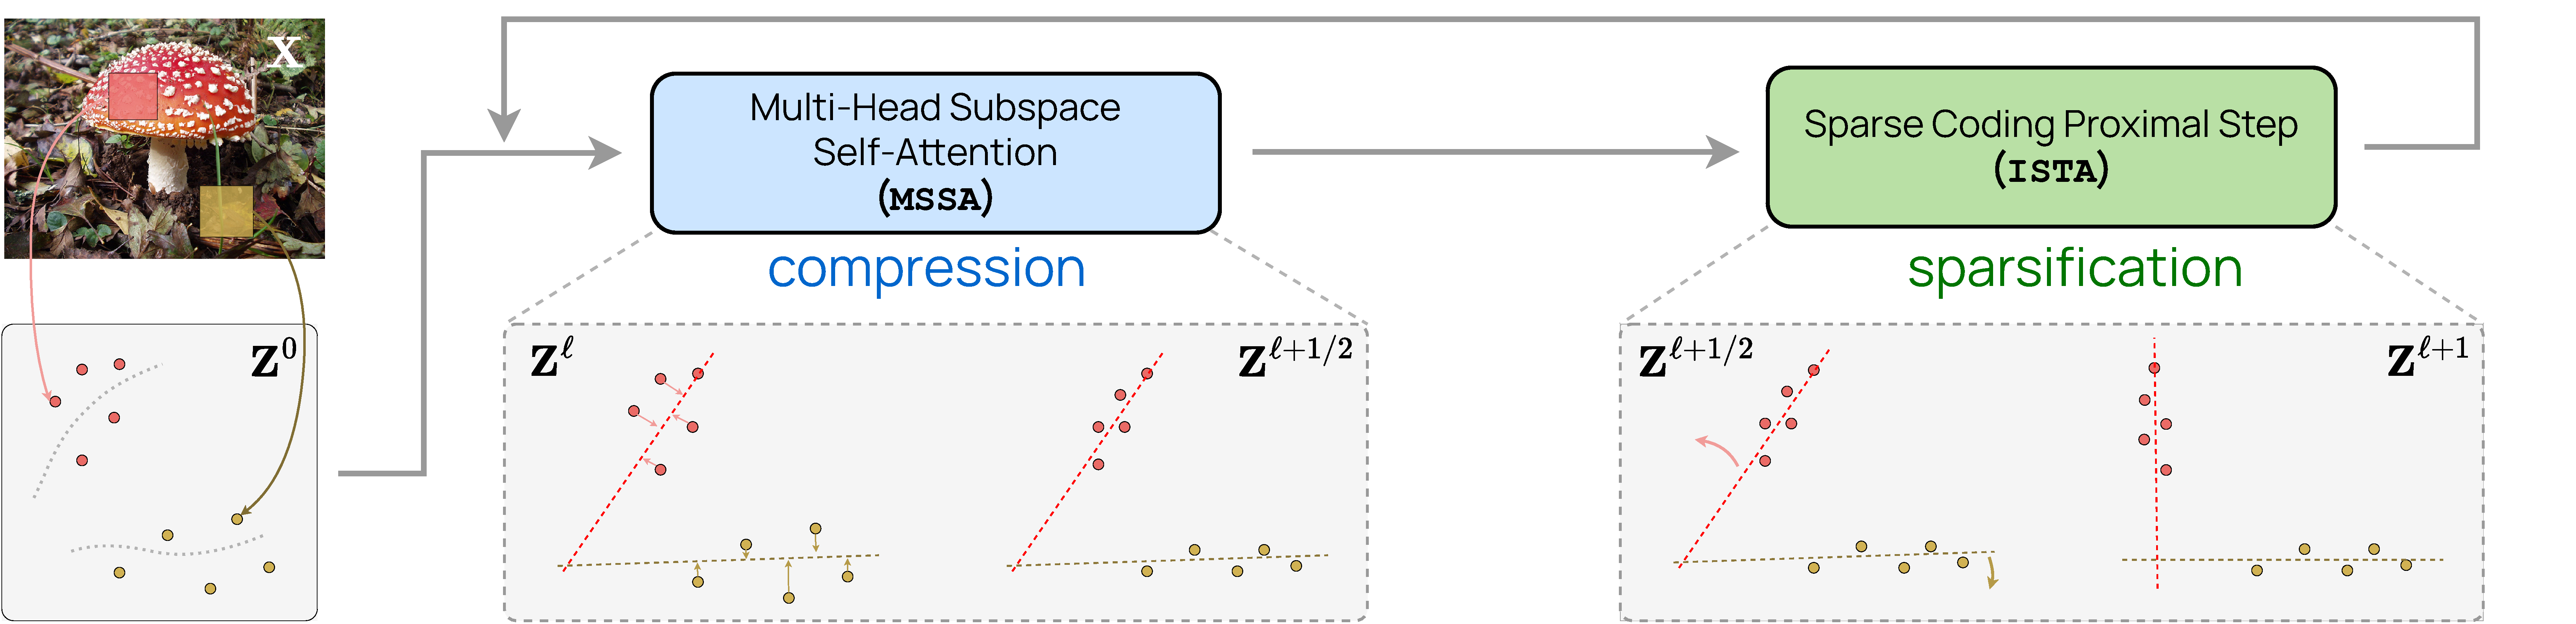
\includegraphics[width=\textwidth]{\toplevelprefix/chapters/chapter4/figs/CRATE_fig1_patches.pdf}
     \vspace{-0.1in}
     \caption{
     \textbf{The `main loop' of the \textsc{crate} white-box deep network design.} 
     After encoding input data as a sequence of tokens $\vZ^0$, \textsc{crate} constructs a deep network that transforms the data to a canonical configuration of low-dimensional subspaces by successive   {\textit{\textbf{compression}}} 
     against a local model for the distribution, generating $\vZ^{\ell+1/2}$, and      {\textit{\textbf{sparsification}}} 
     against a global dictionary, generating $\vZ^{\ell+1}$. 
     Repeatedly stacking these blocks and training the model parameters via backpropagation yields a powerful and interpretable representation of the data.
     }
        \label{fig:crate-diagram}
\end{figure}


\begin{remark}[\textbf{The roles of the forward pass and backward propagation}]\label{sub:forward_backward}
    In contrast to other unrolled optimization approaches such as the ReduNet \cite{chan2021redunet}, we \textit{explicitly model} the distribution of each $\vZ^\ell$ and $\vZ^{\ell + 1/2}$ at each layer, either by a mixture of linear subspaces or sparsely generated from a dictionary. We introduced the interpretation that at each layer \(\ell\), the learned bases for the subspaces \(\vU_{[K]}^{\ell}\) and the learned dictionaries \(\vD^{\ell}\) together serve as a \textit{codebook} or \textit{analysis filter} that encodes and transforms the intermediate representations at each layer \(\ell\). Since the input distribution to layer \(\ell\) is first modeled by \(\vU_{[K]}^{\ell}\) then transformed by \(\vD^{\ell}\), the input distribution to each layer is different, and so we require a separate code book at each layer to obtain the most parsimonious encoding. Parameters of these codebooks (i.e., the subspace bases and the dictionaries), heretofore assumed as being perfectly known, are actually learned from data (say via \textit{backward propagation} within end-to-end training).
    
    Hence, our methodology features a clear conceptual separation between forward ``optimization'' and backward ``learning'' for the so-derived white-box deep neural network. Namely, in its forward pass, we interpret each layer as an operator which, conditioned on a learned model (i.e., a codebook) for the distribution of its input, transforms this distribution towards a more parsimonious representation. In its backward propagation, the codebook of this model, for the distribution of the input to each layer, is updated to better fit a certain (supervised) input-output relationship, as illustrated in Figure \ref{fig:forward-backward}. This conceptual interpretation implies a certain agnosticism of the model representations towards the particular task and loss; in particular, many types of tasks and losses will ensure that the models at each layer are fit, which ensures that the model produces parsimonious representations.
\end{remark}






We now present the empirical performance of the proposed networks \textsc{crate} by measuring their top-1 classification accuracy on ImageNet-1K as well as transfer learning performance on several widely used downstream datasets. 
We summarize the results in Table \ref{tab:crate_comparison_with_sota}. The transfer learning methodology is to fine-tune using cross-entropy loss initializing from the pre-trained networks. 
As the designed white-box transformer architecture leverages parameter sharing in both the attention block (\texttt{MSSA}) and the nonlinearity block (\texttt{ISTA}), the \textsc{crate}{-Base} model (22.80 million) 
has a similar number of parameters to the ViT-Small (22.05 million)~\cite{dosovitskiy2020image}, and less than 30\% of the parameters of an identically configured ViT-Base (86.54 million). 
From Table~\ref{tab:crate_comparison_with_sota}, we find that with a similar number of model parameters, our proposed network achieves similar ImageNet-1K and transfer learning performance as ViT, while having a simple and principled design. Moreover, with the same set of training hyperparameters, we observe promising scaling behavior in \textsc{crate}---we consistently improve the performance by scaling up the model size. To summarize, \textsc{crate} achieve promising performance on real-world large-scale datasets by directly implementing our principled architecture. We will provide more details of the implementation and analysis of the experimental results on image classification in the final application Chapter \ref{ch:applications}.

\begin{figure}[t]
    \begin{subfigure}[t]{0.48\textwidth}
        \centering
        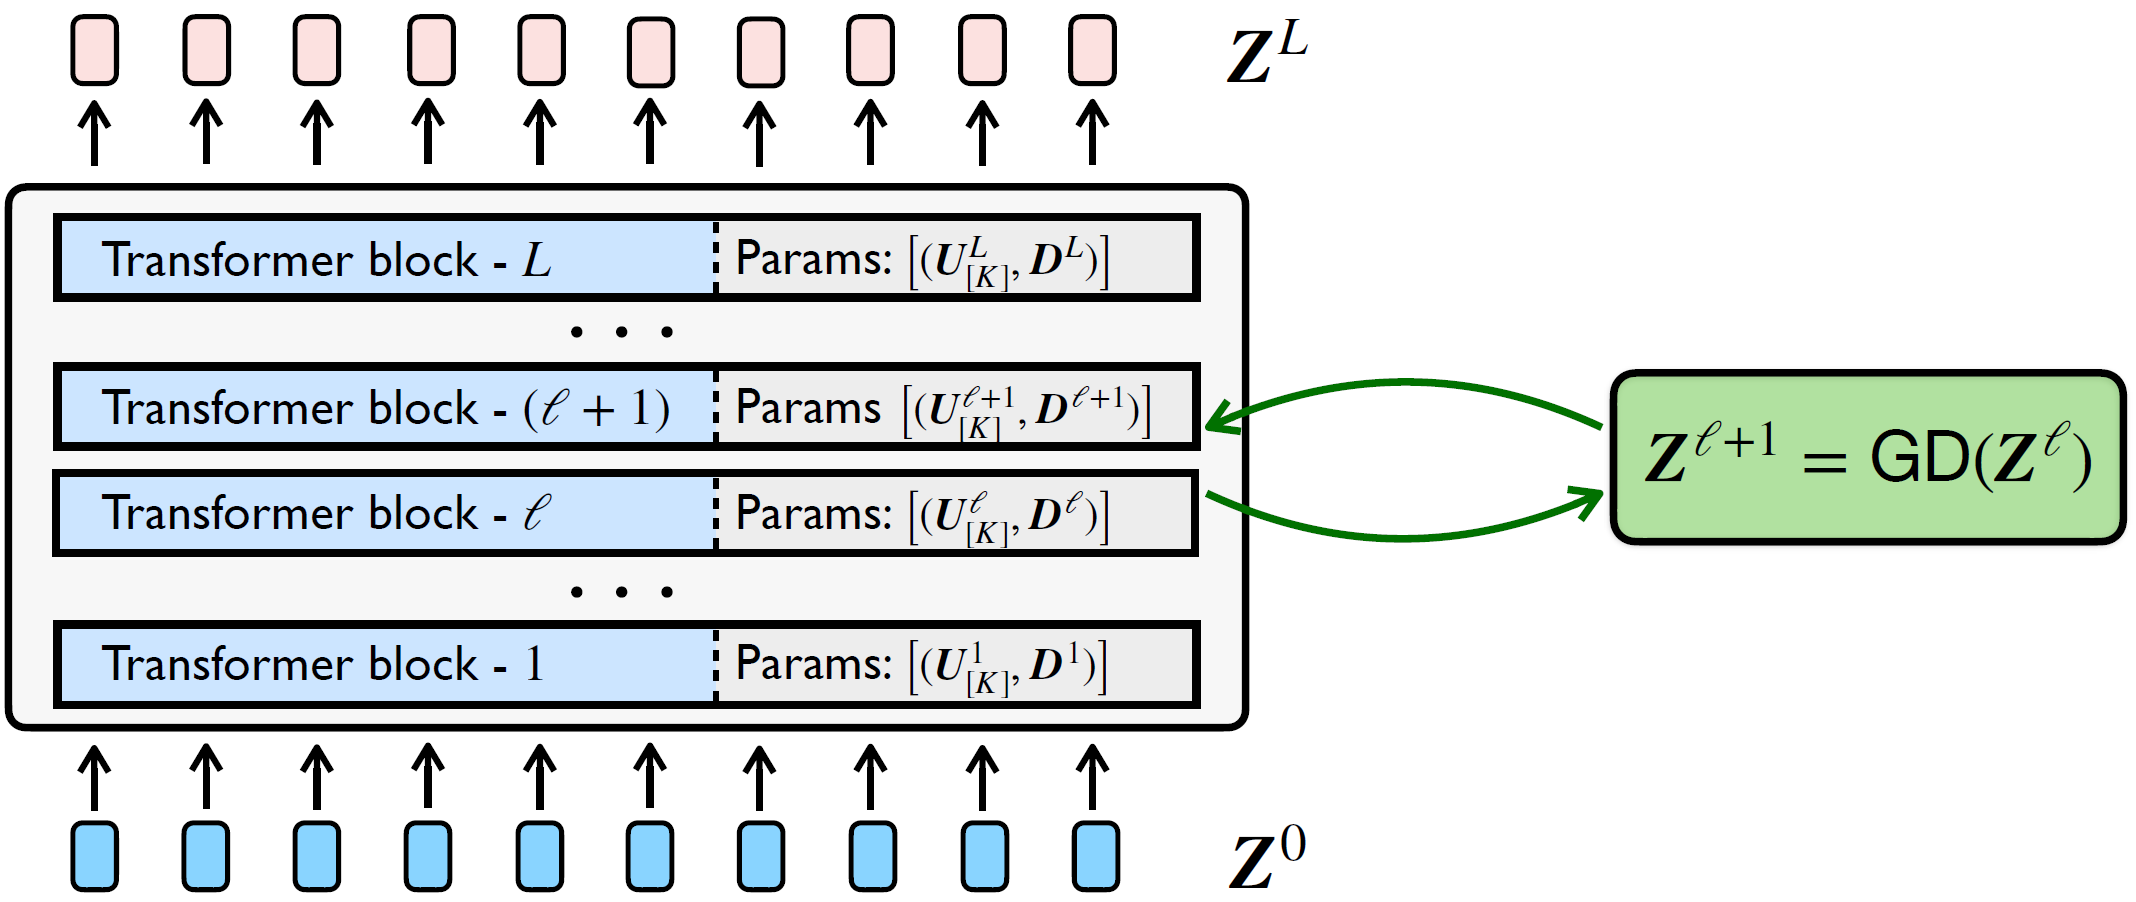
\includegraphics[width=\textwidth]{\toplevelprefix/chapters/chapter4/figs/forward.png}
        \caption{\bf Forward pass}
    \end{subfigure}
    \hfill
    \begin{subfigure}[t]{0.48\textwidth}
        \centering
        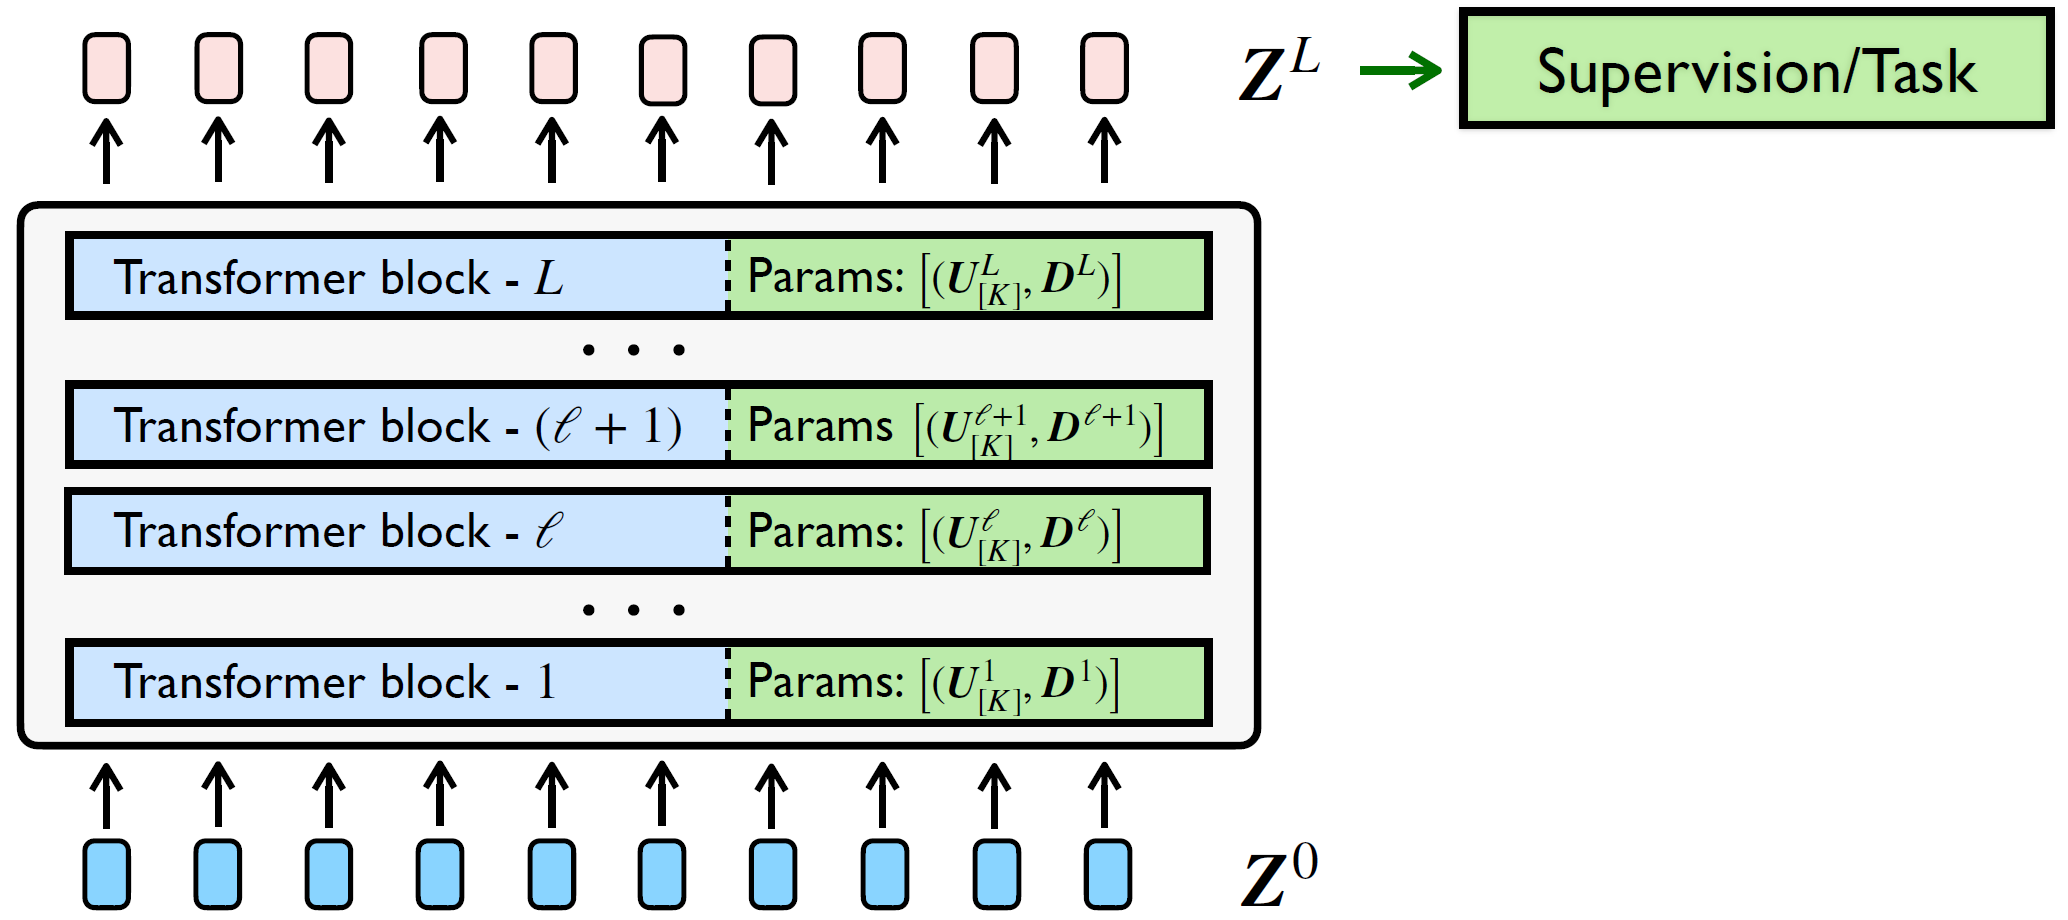
\includegraphics[width=\textwidth]{\toplevelprefix/chapters/chapter4/figs/backward.png}
        \caption{\bf Backward propagation}
    \end{subfigure}
    \caption{\small {\bf The roles of forward pass and backward propagation in deep networks}. (a) Given fixed subspaces and dictionaries $\{(\bm U_{[K]}^{\ell}, \bm D^{\ell})\}_{\ell=1}^L$, each layer performs compression and sparsification on representations in the forward pass; (b) Backpropagation learn subspaces and dictionaries $\{(\bm U_{[K]}^{\ell}, \bm D^{\ell})\}_{\ell=1}^L$ from training data. }
    \label{fig:forward-backward}
\end{figure}


\begin{table*}[t!]
\centering
\caption{\small Top-1 classification accuracy of \textsc{crate} on various datasets with different model scales 
when pre-trained on ImageNet-1K. For ImageNet-1K/ImageNet-1K ReaL, we directly evaluate the top-1 accuracy. For other datasets, we use models that are pre-trained on ImageNet as initialization and the evaluate the transfer learning performance via fine-tuning.}
\label{tab:crate_comparison_with_sota}
\small
    \setlength{\tabcolsep}{13.6pt}
\resizebox{0.98\textwidth}{!}{\begin{tabular}{@{}lcccc|cc@{}}
\toprule
\textbf{Model} & \textsc{crate}{-T}  &  \textsc{crate}{-S} & \textsc{crate}{-B} & \textsc{crate}{-L} & { \color{gray} ViT-T} &  { \color{gray}ViT-S } \\ 
\midrule
\midrule
 \# parameters & 6.09M & 13.12M & 22.80M & 77.64M & { \color{gray} 5.72M} & { \color{gray} 22.05M} \\
\midrule
 ImageNet-1K & 66.7 & 69.2 & 70.8 & 71.3 & { \color{gray} 71.5} & { \color{gray} 72.4} \\
 ImageNet-1K ReaL & 74.0 & 76.0 & 76.5 & 77.4 & { \color{gray} 78.3 } & { \color{gray} 78.4} \\
 \midrule
 CIFAR10 & 95.5 & 96.0 & 96.8 & 97.2 & { \color{gray} 96.6} & { \color{gray} 97.2} \\
 CIFAR100 & 78.9 & 81.0 & 82.7 & 83.6 & { \color{gray} 81.8} & { \color{gray} 83.2}\\
 Oxford Flowers-102 & 84.6 & 87.1 & 88.7 & 88.3 & { \color{gray} 85.1} & { \color{gray} 88.5}\\
 Oxford-IIIT-Pets & 81.4 & 84.9 & 85.3 & 87.4 & { \color{gray} 88.5} & { \color{gray} 88.6} \\
 \bottomrule
\end{tabular}}
\end{table*}



\section{Variants of Deep Architectures by Design} \label{sec:chap4-derive-white-box-transformer-variants}

So far, we wish that we have provided compelling evidence that the role of (popular) deep networks is to realize certain optimization algorithms for minimizing the coding rate (or maximizing the information gain) of the learned representations. However, readers who are familiar with optimization methods might have noticed that the above architectures (the ReduNet or the CRATE) correspond to rather basic optimization techniques. They may have plenty of room for improvement in efficiency or effectiveness. Moreover, if we believe the proposed theoretical framework for interpreting deep networks is correct, it should not only help explain existing architectures, it should guide us develop more efficient and effective architectures. In this section, we show this could be the case: the resulting new architectures are not only fully interpretable but also with guaranteed correctness and improved efficiency. 





\subsection{Attention-Only Transformer Architecture} \label{sub:aot}

In this subsection, we propose a minimalistic transformer architecture consisting of interpretable layers based on the MSSA operator. To derive a fully interpretable transformer architecture with only necessary components,
we contend that the goal of representation learning is to compress a set of noisy initial token representations towards a mixture of low-dimensional subspaces. %
Here, we assume that the initial token representations $\bm Z^{(1)}$ are sampled from a mixture of low-rank Gaussians perturbed by noise as follows: 
\begin{definition}\label{def:MoG}
Let $C_1,\dots,C_K$ be a partition of the index set $[N]$ and $\bm U_k \in \mathcal{O}^{d \times p_k}$ denote the orthonormal basis of the $k$-th subspace for each $k \in [K]$. We say that the token representations $\{\bm z_i \}_{i=1}^N \subseteq \R^d$ are sampled from a mixture of noisy low-rank Gaussian distributions if for each $k \in [K]$,
\begin{align}\label{eq:MoG}
    \bm z_i = \underbrace{\bm U_{k} \bm a_i}_{\bf signal} + \underbrace{\sum_{j \neq k}^K \bm U_j \bm e_{i,j}}_{\bf noise},\ \forall i \in C_k, 
\end{align}
where $\bm{a}_i \overset{i.i.d.}{\sim} \mathcal{N}(\bm{0},\bm{I}_{p_k})$ and $\bm{e}_{i,j} \overset{i.i.d.}{\sim} \mathcal{N}(\bm{0},\delta^2\bm{I}_{p_j})$ for all $i \in C_k$ and $k \in [K]$, $\{\bm{a}_i\}$ and $\{\bm{e}_{i,j}\}$ are respectively mutually independent, and $\{\bm{a}_i\}$ is independent of $\{\bm{e}_{i,j}\}$.         
\end{definition}
This model serves as an idealized framework for approximating token representations in real-world pretrained LLMs. It assumes that the token representations are sampled from a mixture of multiple low-rank Gaussian distributions with noise. Under this model, the goal of representation learning is to compress a set of noisy initial token presentations into the corresponding subspace. In addition, this model aligns well with two well-established hypotheses about the structure of token representations in pretrained large language models: the ``linear representation hypothesis''  \citep{jiang2024origins,park2023linear} and the ``superposition hypothesis'' \citep{elhage2022toy,yun2021transformer}. 

\begin{remark}
    The linear representation hypothesis posits that token representations in LLMs lie in low-dimensional linear subspaces that encode semantic features. Similarly, the superposition hypothesis suggests that these representations can be approximately expressed as a sparse linear combination of these feature vectors. In \Cref{def:MoG}, each basis $\bm U_k$ of the subspaces can be interpreted as a set of semantic features, where each feature corresponds to a specific aspect of the token's meaning. Token representations are then approximately expressed as sparse linear combinations of these subspace bases, capturing the essential semantic components of the token while ignoring irrelevant dimensions. 
\end{remark}

\paragraph{Denoising Operator for Token Representations.} Now, we show that the MSSA operator (see \eqref{eq:Multi-Head-SSA}) can incrementally denoise token representations generated from the above model. Spefically, we consider for each $\ell =1 ,\dots,L$, 
\begin{align}\label{eq:MSSA}
    \bm Z^{(\ell+1)} =  \bm Z^{(\ell)} + \eta \sum_{k=1}^K \bm U_k\bm U_k^T \bm Z^{(\ell)} \varphi \left(\bm Z^{(\ell)^T}\bm U_k\bm U_k^T\bm Z^{(\ell)} \right),
\end{align}
where $\{\bm U_k\}_{k=1}^K$ is defined in \Cref{def:MoG}, $\eta > 0$ is the step size, and $\varphi$ is an element-wise operator, such as soft-max, ReLU, or other functions. To simplify our development, we assume that the subspaces in \Cref{def:MoG} are orthogonal to each other, i.e., $\bm U_k^T\bm U_j = \bm 0$ for all $k \neq j$. Note that this assumption is not restrictive, as in high-dimensional spaces, random low-dimensional subspaces are incoherent to each other with high probability, i.e., $\bm U_k^T\bm U_j \approx \bm 0$ \citep{Wright-Ma-2021}.\footnote{One may straightforwardly generalize our results to non-orthogonal subspaces, with slightly more sophisticated analysis.}   

\begin{figure}[t]
    \begin{subfigure}[t]{0.45\textwidth}
        \centering
        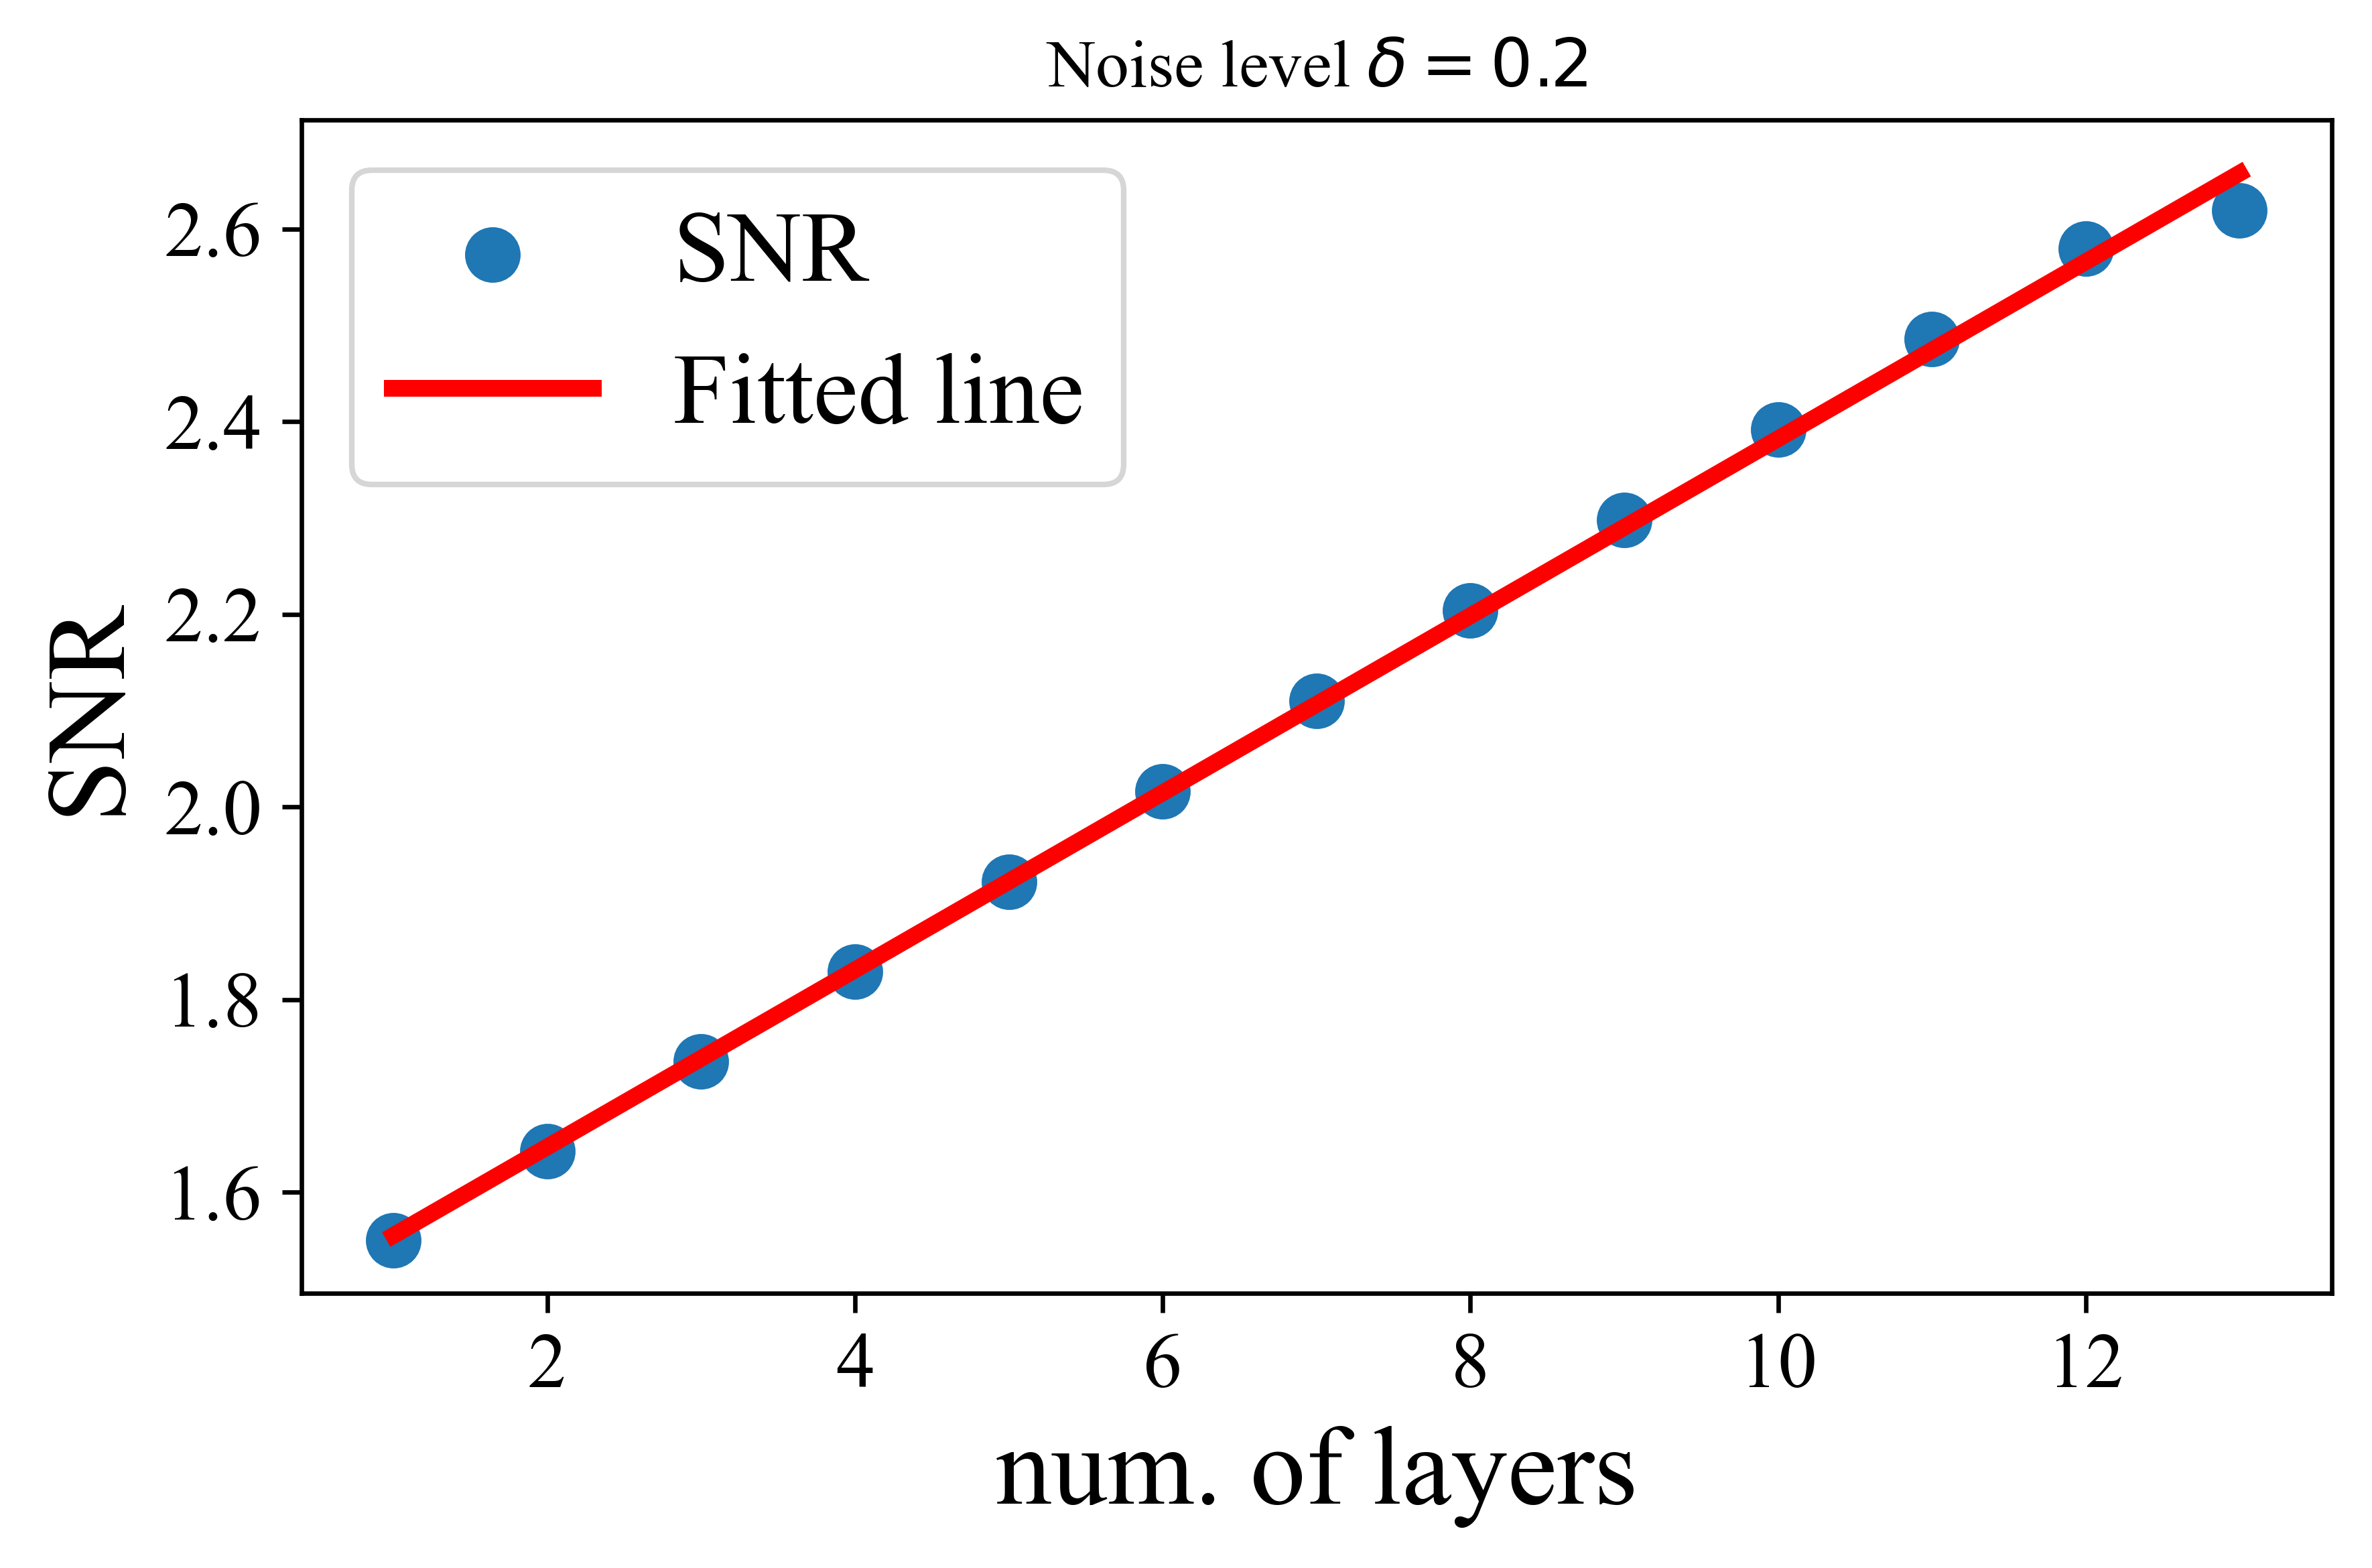
\includegraphics[width=\textwidth]{\toplevelprefix/chapters/chapter4/figs/SNR1.png}
        \caption{Noise level $\delta = 0.2$}
    \end{subfigure}
    \hfill
    \begin{subfigure}[t]{0.45\textwidth}
        \centering
        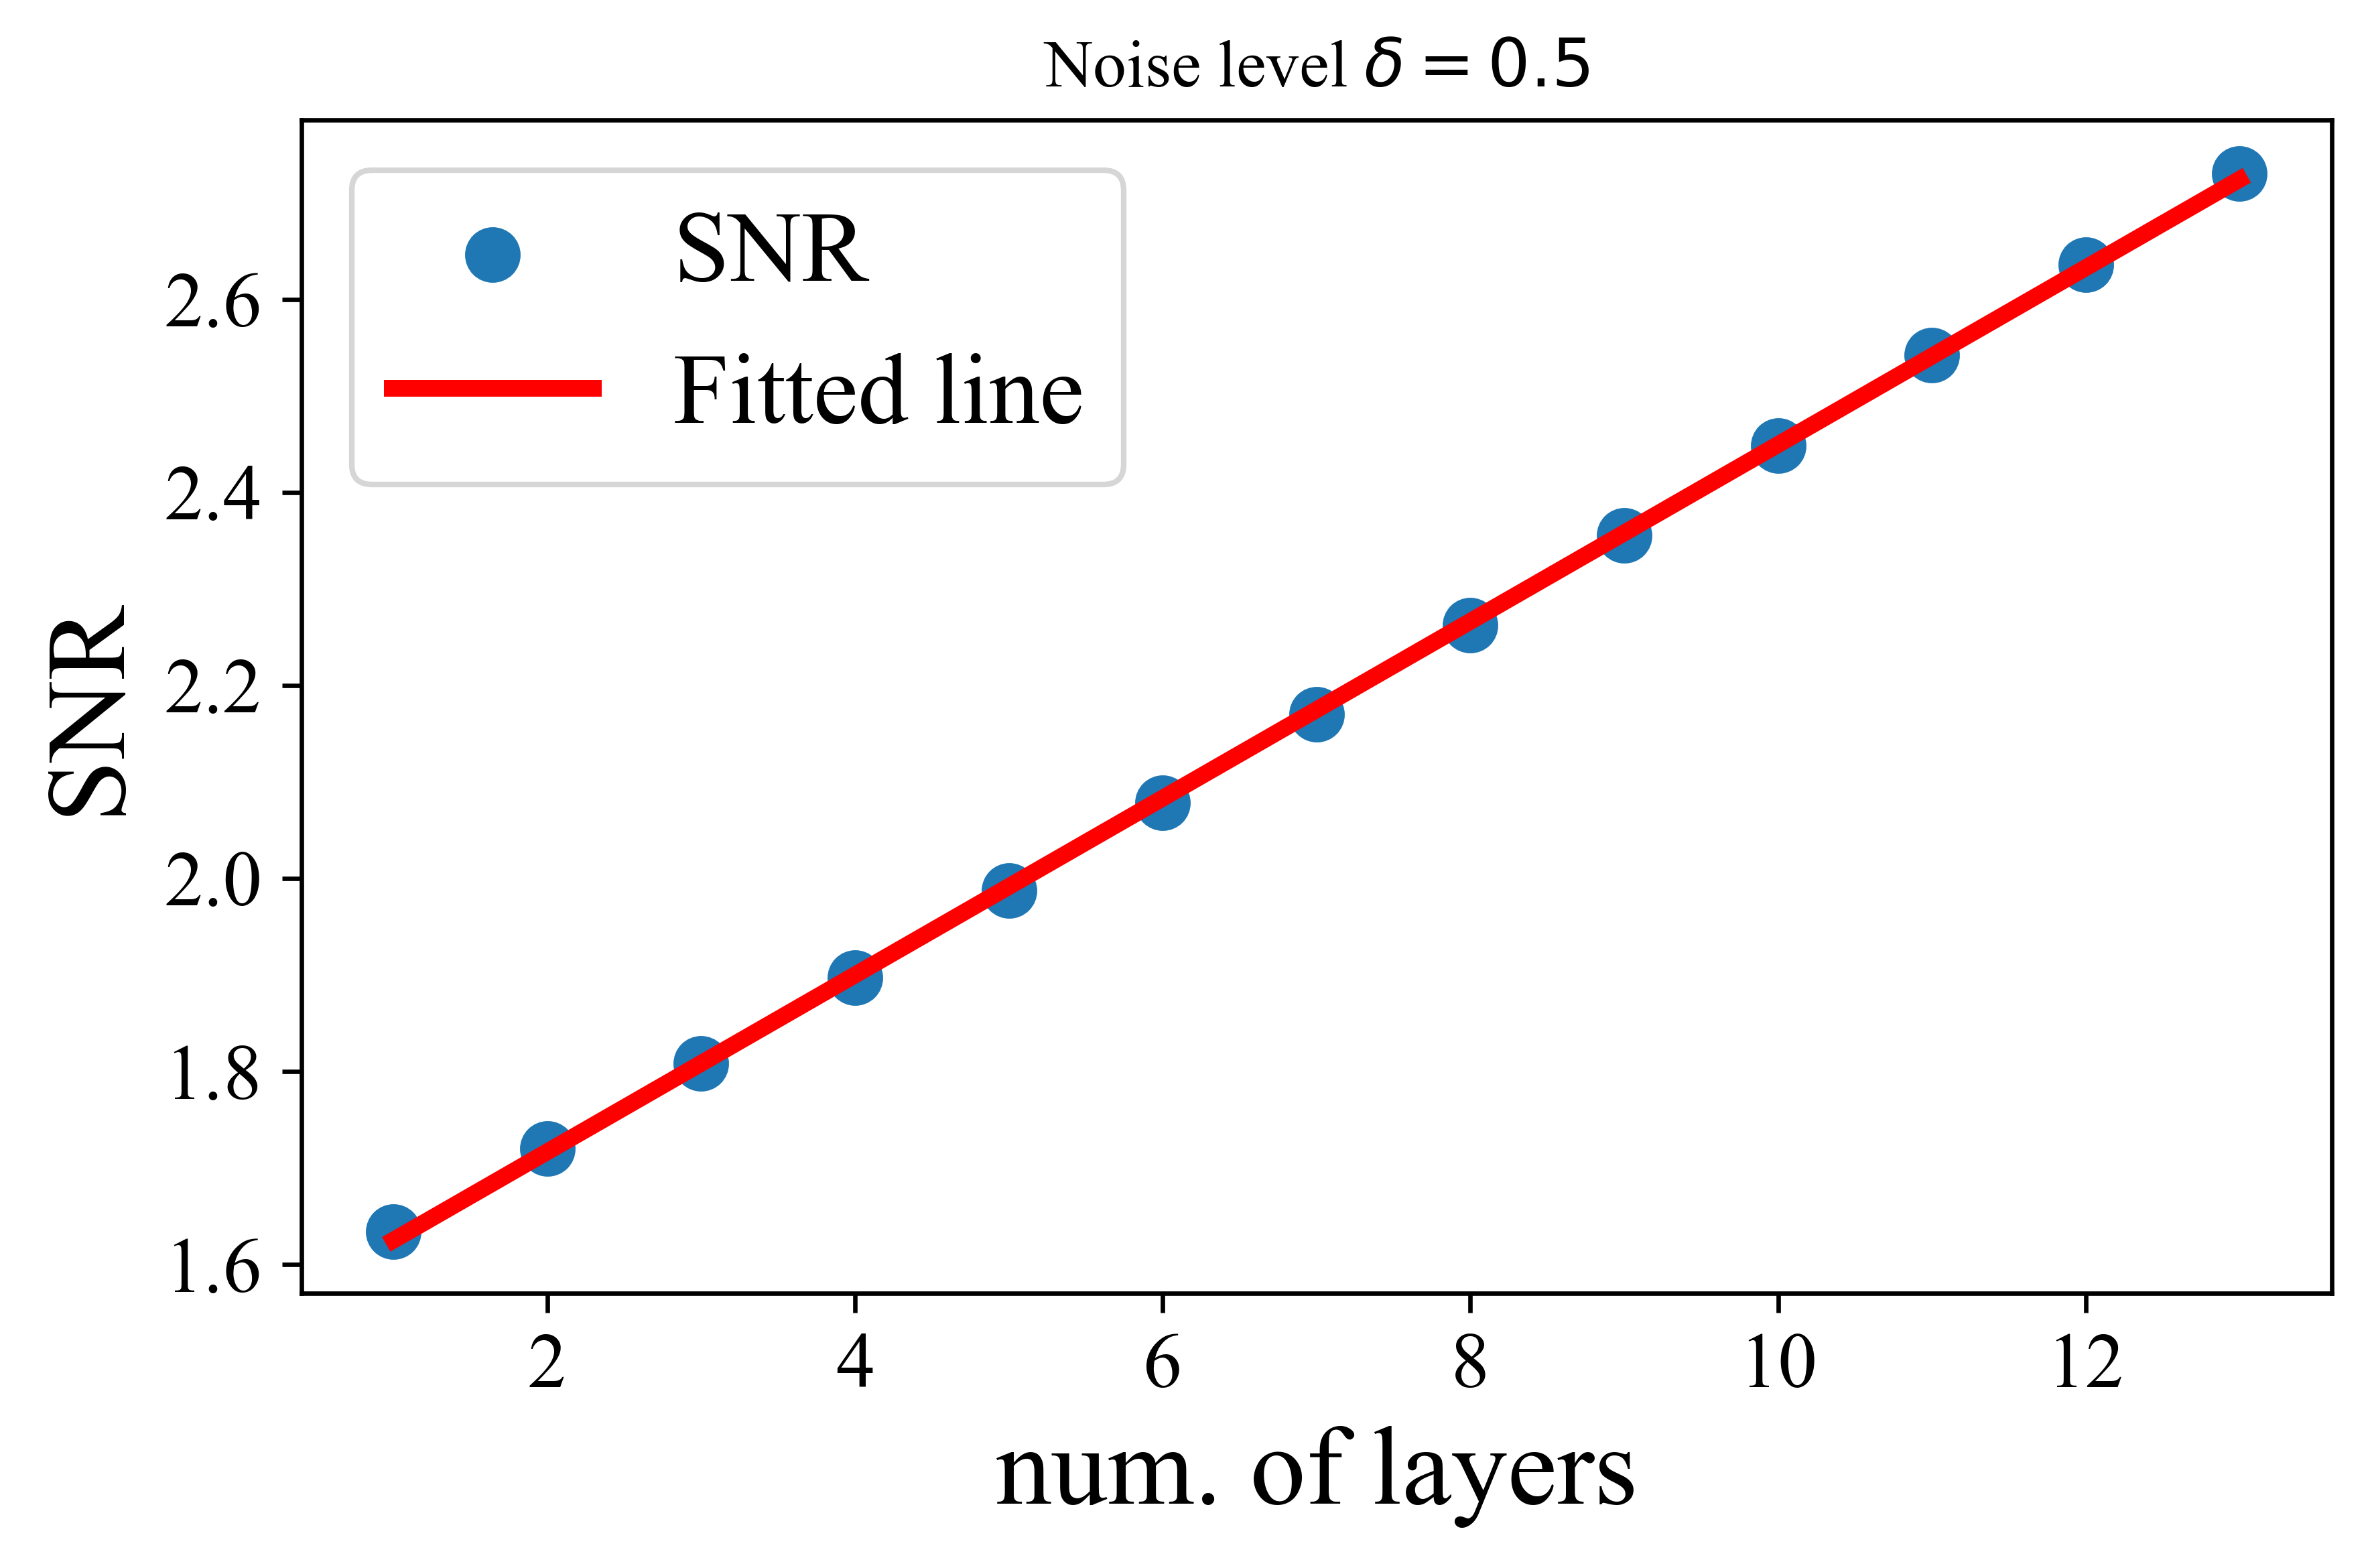
\includegraphics[width=\textwidth]{\toplevelprefix/chapters/chapter4/figs/SNR2.png}
        \caption{Noise level $\delta = 0.5$}
    \end{subfigure}
    \caption{{\bf Denosing performance of the attention-only transformer.} Here, we sample initial token representations from a mixture of low-rank Gassuains in \Cref{def:MoG}. Then, we apply (\ref{eq:MSSA}) to update token representations and report the SNR at each layer.}  \label{fig:MSSA} 
\end{figure} 


Now, let the columns of $\bm Z_k^{(\ell)}$ denotes the token representations from the $k$-th subspace at the $\ell$-th layer. To quantify the denoising capability, we define the signal-to-noise ratio (SNR) for each block of the token representations at the $\ell$-th layer as follows: 
\begin{align}\label{def:SNR}
\mathrm{SNR}(\bm Z_k^{(\ell)}) \doteq  \frac{\|\bm U_k\bm U_k^T\bm Z_k^{(\ell)} \|_F}{\|(\bm I - \bm U_k\bm U_k^T)\bm Z_k^{(\ell)} \|_F},\quad \forall k \in [K].
\end{align}
To simplify our analysis, we assume that $p=p_1=\dots=p_K$, $N_1=\dots=N_K=N/K$, and 
\begin{align}\label{eq:orth}
\begin{bmatrix}
\bm U_1 & \dots & \bm U_K
\end{bmatrix} \in \mathcal{O}^{d\times Kp}. 
\end{align}  

With the above setup, we now characterize the denoising performance of the MSSA operator.

\begin{figure*}[t]
\begin{center}
        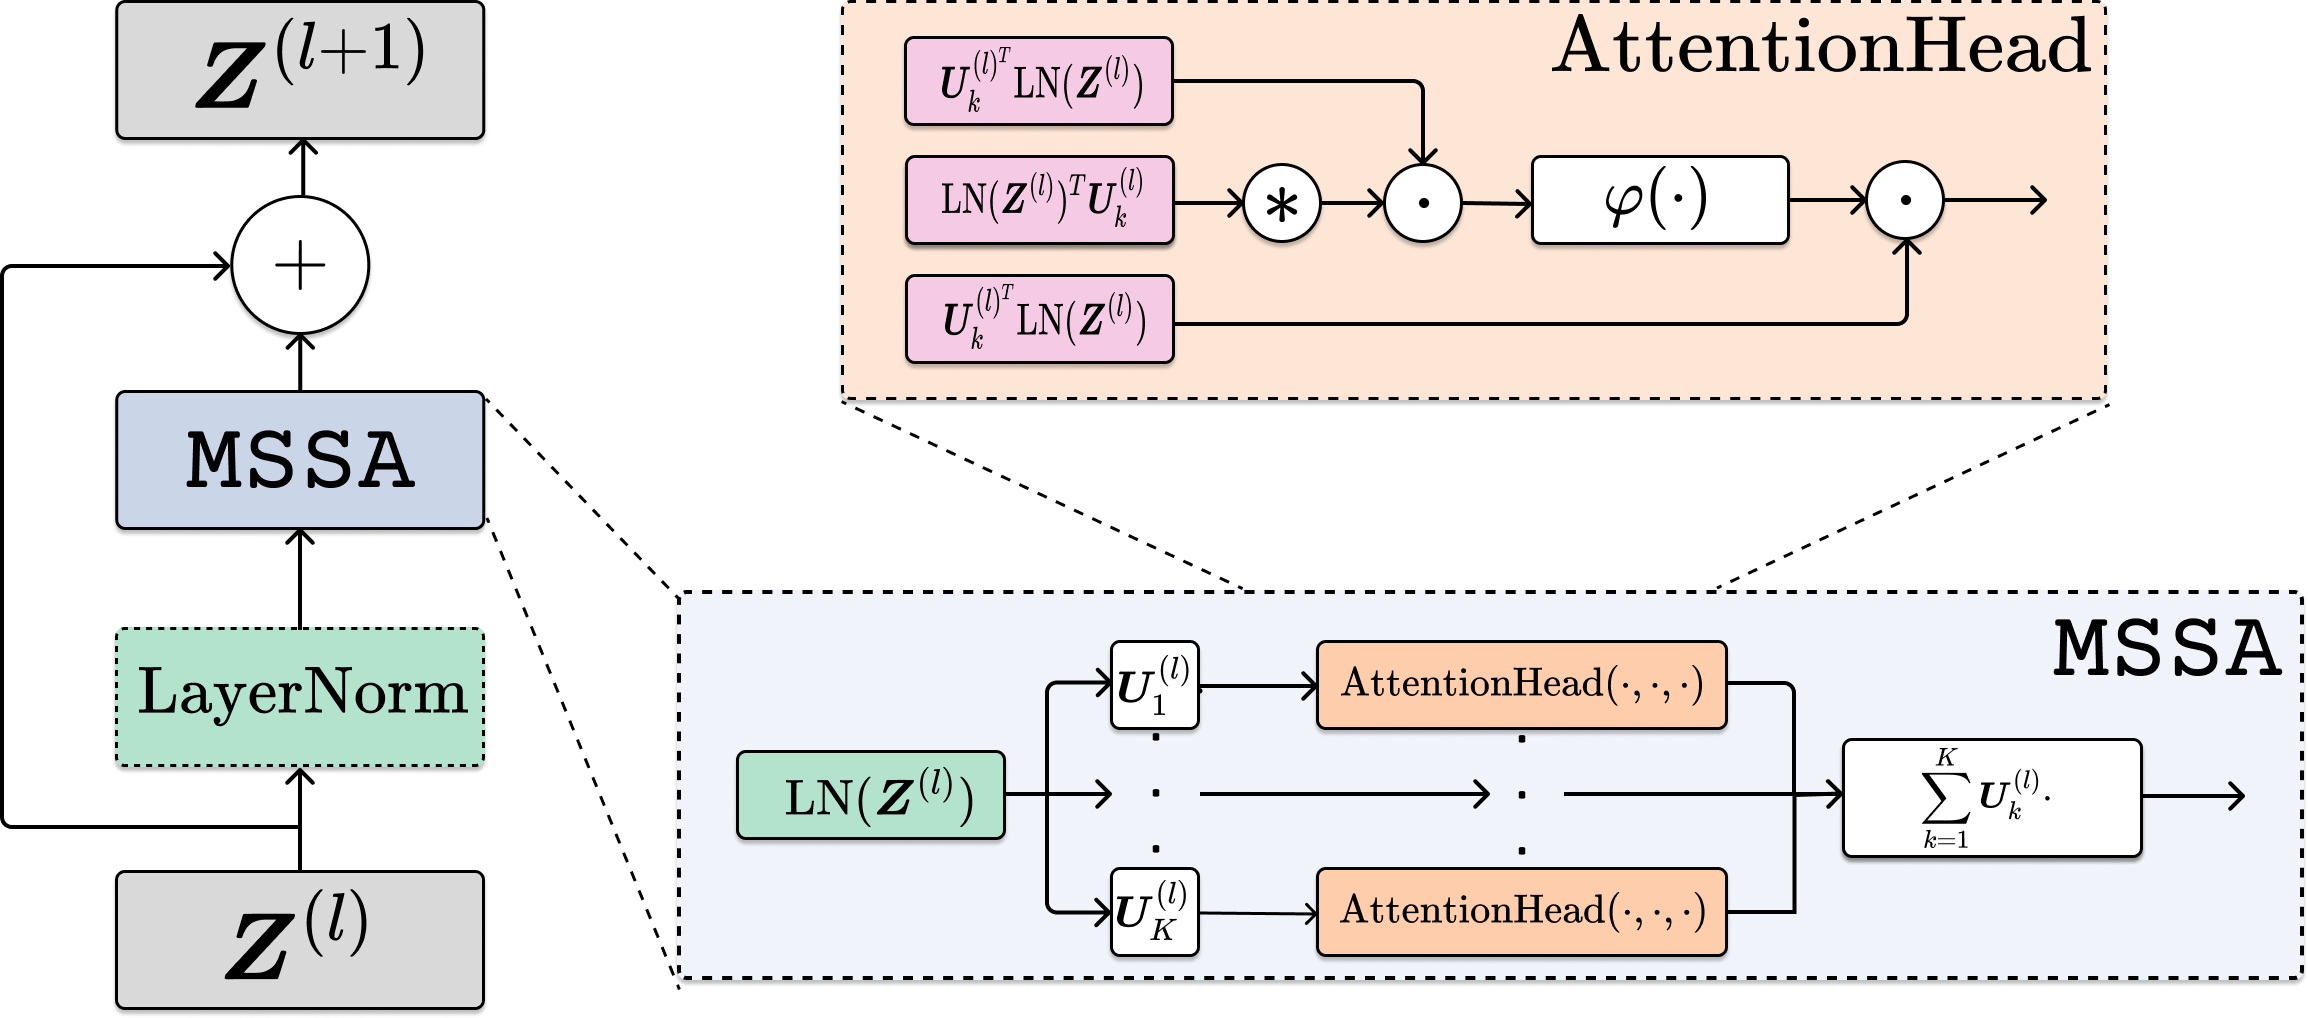
\includegraphics[width=0.75\textwidth]{\toplevelprefix/chapters/chapter4/figs/MSSA.png}
    \caption{\textbf{Details of the attention-only transformer architecture.} Each layer consists of the MSSA operator and a skip connection. In addition, LayeNnorm is included only for language tasks. In practice, backpropagation is applied to train the model parameters using training samples. %
    }\label{fig:transformer}
\end{center} 
\end{figure*}

\begin{theorem}\label{thm:1}
Let $\bm Z^{(1)}$ be defined in \Cref{def:MoG} and $\varphi(\cdot)$ in Eq. (\ref{eq:MSSA}) be 
$\varphi(\bm x) = h\left(\sigma(\bm x)\right)$,
where $\sigma:\R^N \to \R^N$ is the soft-max function and $h:\R^N \to \R^N$ is an element-wise thresholding function with $h(x) = \tau \mathbb{I}\left\{x > \tau\right\}$ for each $i \in [N]$. Suppose that $p \gtrsim \log N$, $\delta \lesssim \sqrt{\log N}/\sqrt{p}$, and 
\begin{align*}
\tau \in \left( \frac{1}{2},  \frac{1}{1+N\exp(-9p/32)} \right].
\end{align*}
For sufficiently large $N$, it holds with probability at least $1-KLN^{-\Omega(1)}$ that for each $\ell \in [L]$, 
    \begin{align}\label{eq:SNR}
        \mathrm{SNR}(\bm Z_k^{(\ell+1)}) = (1+\eta\tau) \mathrm{SNR}(\bm Z_k^{(\ell)}),\ \forall k \in [K]. 
    \end{align}
\end{theorem}
This theorem demonstrates that when the initial token representations are sampled from a mixture of low-rank Gaussian distributions with a noise level $O(\sqrt{\log N}/\sqrt{p})$, we show that each layer of the proposed transformer denoises token representations at a linear rate. This indicates the MSSA operator's efficiency in reducing noise across layers. Notably, our theoretical results are well-supported by experimental observations in \Cref{fig:MSSA}. This theorem provides a theoretical foundation for the practical denoising capability of the transformer architecture derived by unrolling (\ref{eq:MSSA}). 

\begin{remark}
    Under this model, the goal of representation learning is to compress a set of noisy initial token presentations into the corresponding subspace. However, we should point out that in real-world applications, where token representations exhibit more complicated structures, the goal of representation learning is to find a compact and structured representation by compressing token sets. 
\end{remark}


\paragraph{Attention-Only Transformer.} Now, we formally propose an attention-only transformer architecture. Specifically, by unrolling the iterative optimization steps (\ref{eq:MSSA}) as layers of a deep network, we construct a transformer architecture in \Cref{fig:transformer}. Each layer of the proposed architecture only consists of the MSSA operator and a skip connection. For language tasks, we additionally incorporate LayerNorm before the MSSA operator to improve performance. The complete architecture is built by stacking such layers, along with essential task-specific pre-processing and post-processing steps, such as positional encoding, token embedding, and final task-specific head to adapt to different applications. 




Generally speaking, the standard decoder-only transformer architecture is composed of the following key components \cite{vaswani2017attention}: (1)  positional encoding, (2) multi-head QKV self-attention mechanisms, (3) feed-forward MLP networks, (4) layer normalization, and (5) residual connections. In contrast, our proposed transformer architecture adopts a streamlined design by incorporating several key simplications. Specifically, it employs shared-QKV subspace self-attention mechanisms, excludes MLP layers, and reduces the frequency of LayerNorm.










\subsection{Linear-Time Attention: Token Statistics Transformer}\label{sub:tost} 

In this subsection, we propose a new transformer attention operator whose computational complexity scales linearly with the number of tokens based on the coding rate reduction objective.  Specifically, we derive a novel variational form of the MCR$^2$ objective and show that the architecture that results from unrolled gradient descent of this variational objective leads to a new attention module called Token Statistics Self-Attention (\texttt{TSSA}). \texttt{TSSA} has {\em linear computational and memory complexity} and radically departs from the typical attention architecture that computes pairwise similarities between tokens.  Recall from \eqref{eq:MCR pi} that $\bm \Pi = [\bm \pi_1, \ldots, \bm \pi_K] \in \R^{N \times K}$ denotes a stochastic ``group assignment'' matrix (i.e., $\bm \Pi \bm 1 = \bm 1$ and $\Pi_{ik} \geq 0, \  \forall (i,k) \in [N] \times [K]$ ), where $\Pi_{ik}$ denotes the probability of assigning the $i$-th token to the $k$-th group. 

 

\paragraph{A New Variational Form for Coding Rates.} To begin, we consider a general form of MCR$^2$-like objectives based on concave functions of the spectrum of a matrix.  Namely, for a given PSD matrix $\bm M \in \PSD(d)$ and any scalar $c \geq 0$ we have that $\log \det (\I + c \bm M) = \sum_{i=1}^{d} \log( 1 + c \lambda_i(\bm M))$, where $\lambda_i (\bm M)$ is the $i$-th largest eigenvalue of $\bm M$.  Further, note that $\log(1 + c \sigma)$ is a concave non-decreasing function of $\sigma$.  Thus, we describe our results in terms of a more general form of MCR$^2$ based on general spectral functions of PSD matrices of the form $F(\bm M) = \sum_{i=1}^{d} f(\lambda_i(\bm M))$, where $f$ is concave and non-decreasing.  In particular, recall from our above discussion that the attention mechanism arises from unrolling the compression component of MCR$^2$, so we consider a more general MCR$^2$-style compression function:
\vspace{-2mm}
\begin{equation}
    R_{c,f}(\bm Z, \bm \Pi) \doteq \frac{1}{2}\sum_{k=1}^K \frac{N_k}{N} F\left( \frac{1}{N_k}\Z \mathrm{Diag}(\bm \pi_k) \Z^{\top} \right).
    \label{eq:mcr_c_gen}
\end{equation}



For the above objective, we now note the following result:
\begin{theorem}
\label{thm:var_concave}
    Let \(f \colon [0, \infty) \to \R\) be non-decreasing, concave, and obey \(f(0) = 0\), and let \(F \colon \PSD(d) \to \R\) have the form \(F(\bm M) = \sum_{i = 1}^{d}f(\lambda_{i}(\bm M))\). Then for each \(\bm M \in \PSD(d)\) and \(\bm Q \in \O(d)\), we have
    \begin{equation}
        \label{eq:U_bound}
        F(\bm M) \leq  \sum_{i=1}^{d} f\left( (\bm Q^{\top} \bm M \bm Q)_{ii} \right).
    \end{equation}
    Further, the inequality in \eqref{eq:U_bound} is achieved with equality for any $\bm Q$ which diagonalizes $\bm M$, and if $f$ is strictly concave then the inequality in \eqref{eq:U_bound} is achieved with equality \textit{if and only if} $\bm Q$ diagonalizes $\bm M$. 
\end{theorem}

Using the above result, we can replace \eqref{eq:mcr_c_gen} with an equivalent variational objective with form
\vspace{-2mm}
\begin{equation}
    \label{eq:var_comp}
    R^{\rm var}_{c,f} (\Z,\bm \Pi \mid \bm U_{[K]}) \doteq \frac{1}{2}\sum_{k=1}^K \frac{N_k}{N} \sum_{i=1}^{d} f\left(\frac{1}{N_k} (\bm U_{k}^{\top} \Z \mathrm{Diag}(\bm \pi_k) \bm Z^{\top} \bm U_{k})_{ii} \right),
\end{equation}
where the equivalence is in the sense that for an optimal choice of $\{ \bm U_k \in \O(d)\}_{k=1}^K$ matrices as described in \Cref{thm:var_concave} (i.e., orthogonal matrices which diagonalize each $\Z \mathrm{Diag}(\bm \pi_k) \Z^\top $) we will achieve a tight bound with $ R^{\rm var}_{c,f} (\Z,\bm \Pi \mid \bm U_{[K]}) = R_{c,f} (\Z,\bm \Pi)$. Note that in general, achieving this bound would require selecting, for each sampled instance of $\Z$, a new optimal set of $\bm U_{k}$ parameter matrices which diagonalize each $\Z\mathrm{Diag}(\bm \pi_{k})\Z^{\top}$, which is clearly impractical for network architecture. 
Instead, as an alternative viewpoint, rather than considering the data ($\Z$) as fixed and trying to optimize the $\bm U_k$ parameters to achieve the tight variational bound, we can instead take the algorithmic unrolling design principle described above and design an operator to perturb $\Z$ to incrementally minimize $R_{c, f}^{\rm var}(\cdot \mid \bm U_{[K]})$.  To make this point explicit, each variational bound becomes tight when the eigenspaces of $\Z \mathrm{Diag}(\bm \pi_k) \Z
^\top$ align with the columns of $\bm U_k$, so by rotating the appropriate columns of $\Z$ (namely, those which correspond to large entries in $\bm \pi_k$) to align with $\bm U_k$ we can approach a tight variational bound. That is, instead of rotating $\bm U_k$ to align with the data for each instance of $\Z$, we can instead rotate the token features in each $\Z$ to align with $\bm U_k$. 

Following this approach, we compute a gradient descent step on $R_{c,f}^{\rm var}$ w.r.t. $\Z$.
To begin this computation, first let $\bm \pi \in \Re^N$ be any element-wise non-negative vector. Then we have
\begin{equation}\label{eq1:grad Rcf}
\nabla_{\Z} \ \frac{1}{2} \sum_{i = 1}^{d} f(  (\Z \mathrm{Diag}(\bm \pi) \Z^{\top} )_{ii}) %
= \; \mathrm{Diag}(\nabla f[ \Z^{\hada 2} \bm \pi] ) \Z \mathrm{Diag}(\bm \pi),
\end{equation}
where $\nabla f$ is the gradient of $f$, and (recall) $\nabla f[\cdot]$ applies $\nabla f$ to each element of the vector in the bracket. In particular, for $ f(x) = \log(1 + (d/\epsilon^{2}) x)$,  $\nabla f(x) = (d / \epsilon^{2}) (1+ (d / \epsilon^{2}) x)^{-1}$ is simply a non-linear activation. Also, (recall) $N_{k} = \langle \bm \pi_{k}, \bm 1\rangle$. Thus, the gradient of $R^{\rm var}_{c,f}$ w.r.t. $\Z$ is:
\begin{align}\label{eq2:grad Rcf}
    \nabla_{\Z} R^{\rm var}_{c,f}(\Z,\bm \Pi \mid \bm U_{[K]}) =  \frac{1}{n}
    \sum_{k=1}^K \bm U_{k} \underbrace{\mathrm{Diag} \left( \nabla f\left[ (\bm
    U_{k}^{\top} \Z)^{\hada 2}  \frac{\bm \pi_k}{\langle \bm \pi_{k}, \bm 1\rangle} \right] \right)}_{\doteq \bm D(\Z, \bm \pi_{k} \mid \bm U_{k})} \bm U_{k}^{\top} \Z \mathrm{Diag}(\bm \pi_k).
\end{align}
(Note that the $1/N$ constant arises from a $(N_{k}/N)\cdot (1/N_{k}) = 1/N$ constant in each term of the sum.) If we now consider a gradient step w.r.t. the $j$-th token $\z_j$
, we arrive at our proposed incremental compression operator, i.e., our surrogate for a \textit{self attention} + residual operator:
\vspace{-2mm}
\begin{equation}\label{eq:layer-operation-orig}
    \z_j^+ = \z_{j} - \tau \nabla_{\z_{j}}R_{c, f}^{\rm var}(\Z, \bm \Pi \mid \bm U_{[K]}) = \z_j - \frac{\tau}{N} \sum_{k=1}^K \Pi_{jk} \bm U_{k} \bm D(\Z, \bm \pi_{k} \mid \bm U_{k}) \bm U_{k}^{\top} \z_j
\end{equation}
for each \(j \in [n]\), where $\tau > 0$ is a step size parameter for the incremental optimization. Then, we can construct a layer of TOST in \Cref{fig:vcrate-architecture}.  

\begin{figure}[t]
    \centering 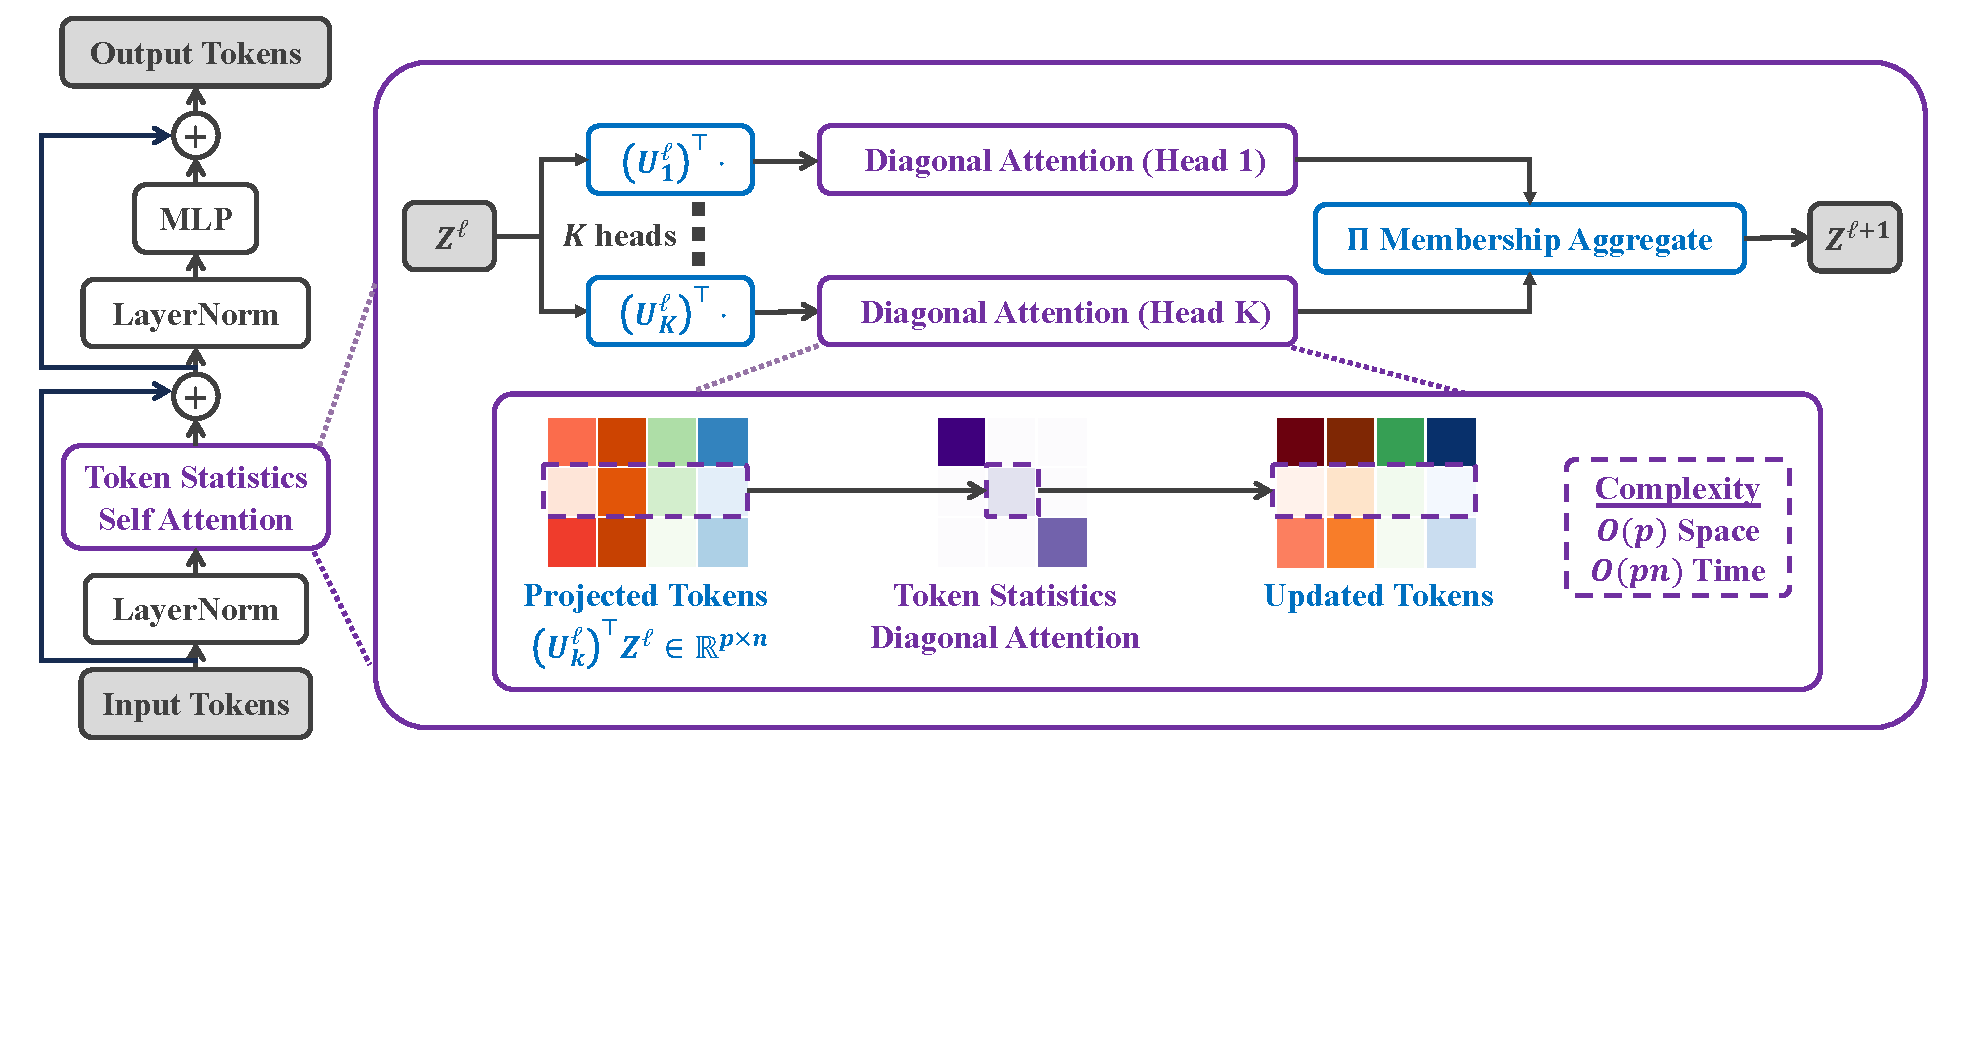
\includegraphics[width=1\textwidth,trim={0 5.0cm 0 0},clip]{\toplevelprefix/chapters/chapter4/figs/V-CRATE.pdf}
    \vspace{-1mm}
    \caption{\small \textbf{One layer $\ell$ of the proposed Token Statistics Transformer (ToST).} Notably, the self-attention of ToST transforms tokens $\Z^{\ell}$ efficiently to $\Z^{\ell+1}$, via multiplying each row of the projected token by \textit{only a scalar}. This leads to reduced complexity of the attention: it has $O(p)$ space and $O(pn)$ time complexity, where $p$ is the dimension of the projected tokens of each head, and $n$ is the number of tokens.
    }
    \label{fig:vcrate-architecture}
\end{figure}

\paragraph{Model interpretation.} Given the proposed attention operator in \eqref{eq:layer-operation-orig}, first recall that the rows of $\bm\Pi$ are non-negative and sum to 1
, so our operator takes a weighted average of $K$ ``attention head''-esque operators and then adds a residual connection. Using that \(\sum_{k = 1}^{K}\Pi_{jk} = 1\), we can rewrite \eqref{eq:layer-operation-orig} as: %
\vspace{-2mm}
\begin{equation}
\label{eq:z_up}
    \z_j^+ = \sum_{k=1}^K \Pi_{jk} \Big[ \z_j \underbrace{- \frac{\tau}{n} \bm U_{k} \bm D(\Z, \bm \pi_{k} \mid \bm U_{k}) \bm U_{k}^{\top}}_{\text{action of one attention head}} \z_j \Big].
\end{equation}
That is, we can view each attention head as first projecting the token features
onto the basis $\bm U_{k}$ via multiplying by $\bm U_k^\top$, multiplying by the
diagonal matrix $\bm D(\Z, \bm \pi_{k} \mid \bm U_{k})$ (abbreviated as \(\bm
D_{k}\)), projecting back into the standard basis via multiplying by $\bm
U_{k}$, and subtracting this from the original token features via the residual
connection. The core aspect of our attention layer is the computation of $\bm
D_{k}$.  Namely, \(\Pi_{jk} \geq 0\), so $\bm \pi_k / \langle \bm \pi_{k}, \bm
1\rangle \in \Re^N$ forms a probability distribution over which tokens belong to
the $k^\text{th}$ group.  As a result, $(\bm U^\top_k \Z)^{\hada 2} \bm \pi_k / \langle \bm \pi_{k}, \bm 1\rangle$ estimates the second moment of $\bm U_k^\top \Z$ under the distribution given by $\bm \pi_k /  \langle \bm \pi_{k}, \bm 1\rangle$.  Further, since $f$ is a concave non-decreasing function, $\nabla f(x)$ monotonically decreases towards $0$ as $x$ increases, so the entries of $\bm D_{k}$ (which have form $\nabla f(x)$) achieve their maximum at $x=0$ %
and decay monotonically to $0$ as $x$ increases.

From this, we arrive at the core interpretation of our attention head + residual
operators $[\I - (\tau/n)\bm U_{k}\bm D_{k}\bm U_{k}^{\top}]$.  Namely, this
operator does an approximate low-rank data-dependent projection, where
directions which have a large amount of ``power'' after the projection $\bm
U_k^\top \Z$ (i.e., directions which have a large second moment $(\bm
U_{k}^{\top}\Z)^{\hada 2}\bm \pi_k / \langle \bm \pi_{k}, \bm 1\rangle$) are preserved, while directions which do not are suppressed. To see this, recall that the entries of $\bm D_k$ decrease monotonically to 0 as the second moment increases, so for directions with large second moments the attention + residual operator acts largely as the identity operator.  Conversely, for directions with a small second moment, our operator subtracts a projection of the tokens along those directions, resulting in those directions being suppressed. Compared to the standard self-attention operator, our method clearly does not compute any pairwise similarities between tokens. Rather, the interactions between the tokens in $\Z$ impact the operator solely through their contribution to the second moment statistic used to construct the $\bm D_{k}$'s.  Nevertheless, similar to the standard self-attention operator, our method still has a clear interpretation as performing a form of compression towards a data-dependent low-rank structure, in the sense that it performs an approximate low-rank projection, where the specific directions that are suppressed are those which are not strongly aligned with other tokens in the group.

\paragraph{Practical Implementation Details.} Having introduced our proposed attention operator, we now discuss further practical considerations.  First, until this point in the presentation, we have avoided discussion of how tokens are ``grouped'' into various attention heads via the $\bm\Pi$ matrix, but clearly a means of constructing $\bm\Pi$ is needed to implement our method.  Additionally, our variational form in \Cref{thm:var_concave} requires the $\bm U$ matrices to be square and orthogonal, but one would ideally like to use smaller matrices (i.e., reduce the number of columns in $\bm U$) for efficiency as well as drop the orthogonality constraints. 

In practice, we do not enforce the orthogonality constraints. To reduce the number of columns in the $\bm U$ matrices, we note that similar to CRATE \citep{yu2023white}, if we assume the features $\bm Z$ within group \(k\) are (approximately) clustered around a low-dimensional subspace --- say of dimension \(p\) --- then the within-group-\(k\) covariance \(\Z\mathrm{Diag}(\bm \pi_{k})\Z^{\top}\) is low-rank, where recall that \cite{yu2020learning} shows that the optimal geometry of $\Z$ will be for each group to be a low-rank subspace, orthogonal to the other groups. We can thus explicitly find a low-dimensional orthonormal basis for the image of this covariance, i.e., the linear span of the data in group \(k\). If the dimension is $p \leq d$, the basis can be represented by a $d\times p$ orthogonal matrix $\bm U_k \in \O(d, p)$. In this case, we can more efficiently upper-bound \(R_{c,f}\) using these low-rank orthogonal basis matrices. To show this, we use a more general version of \Cref{thm:var_concave}  to yield the following corollary.
\begin{corollary}\label{cor:var_concave_logdet}
    Let \(f \colon [0, \infty) \to \R\) be non-decreasing, concave, and obey \(f(0) = 0\), and let \(F \colon \PSD(p) \to \R\) have the form \(F(\bm M) = \sum_{i = 1}^{p}f(\lambda_{i}(\bm M))\). Let \(\Z\), \(\bm \Pi\) be fixed. Then, for all \(\bm U_{1}, \dots, \bm U_{K} \in \O(d, p)\) such that \(\mathrm{image}(\Z\diag(\bm \pi_{k})\Z^{\top}) \subset \mathrm{image}(\bm U_{k})\) for all \(k \in [K]\), we have
    \begin{equation}
        R_{c, f}(\Z, \bm\Pi) \leq R_{c, f}^{\rm var}(\Z, \bm\Pi \mid \bm U_{[K]}), 
    \end{equation}
     where \(R_{c, f}^{\rm var}\) is formally defined in \eqref{eq:var_comp}. Equality holds if \(\bm U_{k}\) diagonalizes \(\Z\diag(\bm \pi_{k})\Z^{\top}\) for each \(k \in [K]\), and if \(f\) is strongly concave then this equality condition becomes an ``if and only if.''
\end{corollary}

The final step to define our attention operator is to estimate the group membership $\bm\Pi$. For this we posit a simple model of how each feature \(\z_{j}\) deviates from its supporting subspace and then find the optimal subspace assignment. \cite{yu2023white} show that if we independently model each \(\z_{j}\) as belonging to a low-dimensional Gaussian mixture model, where each Gaussian has a covariance matrix with identical spectrum and is supported on a subspace with orthonormal basis \(\bm U_{k}\), plus independent Gaussian noise with covariance \(\eta \I\), then the posterior probability that each token \(\z_{j}\) belongs to each subspace is given by the assignment matrix \(\bm \Pi = \bm \Pi(\bm Z \mid \bm U_{[K]})\) as follows:
\begin{align}\label{eq:pi}
    \bm \Pi = \begin{bmatrix} \boldsymbol{\nu}(\z_1 \mid \bm U_{[K]})^\top \\ \vdots \\ \boldsymbol{\nu}(\z_n \mid \bm U_{[K]})^\top \end{bmatrix}, \quad
\text{where} \quad 
\boldsymbol{\nu}(\z_j \mid \bm U_{[K]}) \doteq \operatorname{softmax}\left( \frac{1}{2\eta} \begin{bmatrix} \|  \bm U_{1}^{\top} \z_j \|_2^2 \\ \vdots \\ \| \bm U_{K}^{\top} \z_j \|_2^2 \end{bmatrix} \right), \quad \forall j \in [n],
\end{align}
where $\eta$ becomes a learnable temperature parameter. Thus, given an input feature \(\Z\), we estimate \(\bm\Pi\) using \eqref{eq:pi} and then compute the attention operator.  Combining the construction of $\bm\Pi$ in \eqref{eq:pi} with 
\eqref{eq:layer-operation-orig}, we obtain the {\em Token Statistics Self-Attention} operator: 
\begin{equation}
    \label{eq:tssa}
   \texttt{TSSA}(\Z \mid \bm U_{[K]}) \doteq -\frac{\tau}{n}\sum_{k = 1}^{K}\bm U_{k}\bm D(\Z, \bm\pi_{k} \mid \bm U_{k})\bm U_{k}^{\top}\Z\diag(\bm \pi_{k}),
\end{equation}
where \(\bm\pi_{k}\) are the columns of \(\bm\Pi = \bm\Pi(\Z \mid \bm U_{[K]})\) defined in \eqref{eq:pi} and \(\bm D\) is defined in \eqref{eq2:grad Rcf}. 




\section{Summary and Notes}




The materials presented in this chapter are based on a series of recent works on this topic, including \cite{chan2021redunet, wang2024global, wang2025attention, wu2025token, yu2023white}. These contributions encompass both theoretical advances and practical methodologies for constructing interpretable deep networks through unrolled optimization. Many of the key results and proofs discussed in this chapter are derived directly from, or inspired by, these foundational works. 


The idea of unrolling an optimization algorithm to construct a neural network traces back to the seminal work \cite{gregor2010learning}. In this work, the authors demonstrated that sparse coding algorithms—such as the Iterative Shrinkage-Thresholding Algorithm (ISTA)—can be unrolled to form multilayer perceptrons (MLPs), effectively bridging iterative optimization and neural network design. Notably, \cite{monga2019algorithm} demonstrated that such unrolled networks are more interpretable, parameter-efficient, and effective compared to generic networks. In this chapter, we build on this perspective to develop principled, white-box deep network architectures by unrolling optimization algorithms that are designed to minimize well-motivated objectives—such as the (sparse) rate reduction objective introduced earlier. This approach not only clarifies the role of each layer in the network but also offers theoretical grounding for architectural choices, moving beyond empirical trial-and-error toward interpretable and goal-driven design.  In the following, we compare conventional DNNs, which are typically constructed through empirical design and heuristic tuning, with our mathematically grounded ReduNet architectures: 

\begin{center}
\begin{tabular}{| l || c | c |}
\hline
  & Conventional DNNs & ReduNets\\ [0.5ex]
  \hline \hline
Objectives & input/output fitting & information gain\\ [0.5ex]
  \hline
Deep architectures & trial \& error & iterative optimization \\  [0.5ex]
\hline
Layer operators & empirical & projected gradient \\  [0.5ex]
\hline
Shift invariance & CNNs+augmentation & invariant ReduNets \\  [0.5ex]
\hline
Initializations & random/pre-design & forward unrolled \\ [0.5ex]
\hline
Training/fine-tuning & back prop & forward/back prop\\ [0.5ex]
\hline
Interpretability & black box & white box \\ [0.5ex]
\hline
Representations & hidden/latent & incoherent subspaces \\ [0.5ex]
\hline
\end{tabular}
\end{center}




\section{Exercises and Extensions}


\begin{exercise}
    Let $\bm Z = [\bm Z_1,\dots,\bm Z_K] \in \R^{d\times m}$ with $\bm Z_k \in \R^{d\times m_k}$ for each $k \in [K]$. For some $\alpha > 0$, let 
    \begin{align*}
        R(\bm Z) = \log\det\left(\bm I + \alpha\bm Z\bm Z^T \right).
    \end{align*}
1. Given any direction $\bm D \in \R^{d\times m}$, please show that $\nabla R(\bm Z) = \alpha\bm X^{-1}\bm Z$ and 
    \begin{align*}
 \nabla^2 R(\bm Z)[\bm D, \bm D] =\alpha \mathrm{Tr}\left( \bm X^{-1}\bm D\bm D^T\right) - \frac{\alpha^2}{2}\mathrm{Tr}\left(\bm X^{-1}\left( \bm Z\bm D^T+\bm D\bm Z^T\right) \bm X^{-1}\left( \bm Z\bm D^T+\bm D\bm Z^T\right)\right),
    \end{align*}
    where $\bm X \doteq \bm I + \alpha\bm Z\bm Z^T$. {\em Hint:} Note that
    \begin{align*}
        \nabla^2 R(\bm Z)[\bm D, \bm D] \doteq \left\langle \lim_{t \to 0} \frac{\nabla R(\bm Z+ t\bm D) - \nabla R(\bm Z)}{t}, \bm D \right\rangle. 
    \end{align*}

\noindent
2. Please show that 
\begin{align*}
    R(\bm Z) \le \sum_{k=1}^K \log\det\left(\bm I + \alpha\bm Z_k\bm Z_k^T \right),
\end{align*}
where the equality holds if and only if $\bm Z_k^T\bm Z_l = \bm 0$ for all $k \neq l \in [K]$. 
\medskip 

\noindent 
3. Given some $\alpha >0$, let $\alpha_k=m\alpha/m_k$ for each $k \in [K]$. Please derive the closed-form for the first-order critical point of the following function: 
\begin{align*}
    f(\bm Z_k) = \frac{1}{2}\log\det\left(\bm I + \alpha\bm Z_k\bm Z_k^T \right) - \frac{m_k}{2m}\log\det\left(\bm I + \alpha_k \bm Z_k\bm Z_k^T \right) - \frac{\lambda}{2}\|\bm Z_k\|_F^2. 
\end{align*}
{\em Hint:} Let $r_k=\mathrm{rank}(\bm Z_k)$. Consider the following singular value decomposition of $\bm Z_k$: 
\begin{align*}
    \bm Z_k = \bm P_k\bm \Sigma_k\bm Q_k^T = \begin{bmatrix}
        \bm P_{k,1} & \bm P_{k,2}
    \end{bmatrix} \begin{bmatrix}
        \tilde{\bm \Sigma}_{k} & \bm 0 \\
        \bm 0 & \bm 0
    \end{bmatrix} 
    \begin{bmatrix}
        \bm Q_{k,1}^T \\ \bm Q_{k,2}^T
    \end{bmatrix}, 
\end{align*}
where $\bm P_k \in \mathcal{O}^d$ with $\bm P_{k,1} \in \R^{d\times r_k}$ and  $\bm P_{k,2} \in \R^{d\times (d-r_k)}$, $\bm \Sigma_k \in \R^{d\times m_k}$ with $\tilde{\bm \Sigma}_{k} \in \R^{r_k\times r_k}$ being a diagonal matrix, and  $\bm Q_k \in \mathcal{O}^{m_k}$ with $\bm Q_{k,1} \in \R^{m_k\times r_k}$ and  $\bm P_{k,2} \in \R^{m_k \times (m_k-r_k)}$. 
\medskip 

\end{exercise}


\begin{exercise}[Neumann series for matrix inverse]\label{ex:neumannn} 
Let $\bm A \in \mathbb{R}^{n\times n}$. If $\|\bm A\| < 1$, please show 
\begin{align}\label{eq:neumann}
    \left( \bm I - \bm A\right)^{-1} = \sum_{k=1}^\infty \bm A^k.  
\end{align}
{\em Hint:} The proof consists of two steps. \\
(i) {\bf Step 1}: Please show that the infite series $\sum_{k=1}^\infty \bm A^k$ converges when $\bm A < 1$ using $\|\bm A^k\| \le \|\bm A\|^k$. \\
(ii) {\bf Step 2}: Compute the matrix product $(\bm I - \bm A) \sum_{k=1}^\infty \bm A^k$. 
\end{exercise}


\begin{exercise}
    Please compute the gradients in \eqref{eq1:grad Rcf} and \eqref{eq2:grad Rcf}. 
\end{exercise}


\begin{exercise}
    Please show \Cref{cor:var_concave_logdet} when $Kp \le d$. 
\end{exercise}

\end{document}
